\documentclass{article}
\usepackage{listings}
\usepackage{verbatim}
\lstset{
    frame=single,
    breaklines=true
}
\usepackage{geometry}
\geometry{margin=1in}		%set margins

\usepackage{graphicx}		%need for images
\usepackage{float}			%need for arranging graphics and tables


\title{ECG 782 HW 2}
\date{2015-09-29}
\author{Carlo Lopez-Tello}

\begin{comment}

how to paste code

\lstinputlisting[language=Octave]{Q1/histEqualize.m}

how to paste image

\begin{figure}[H]
	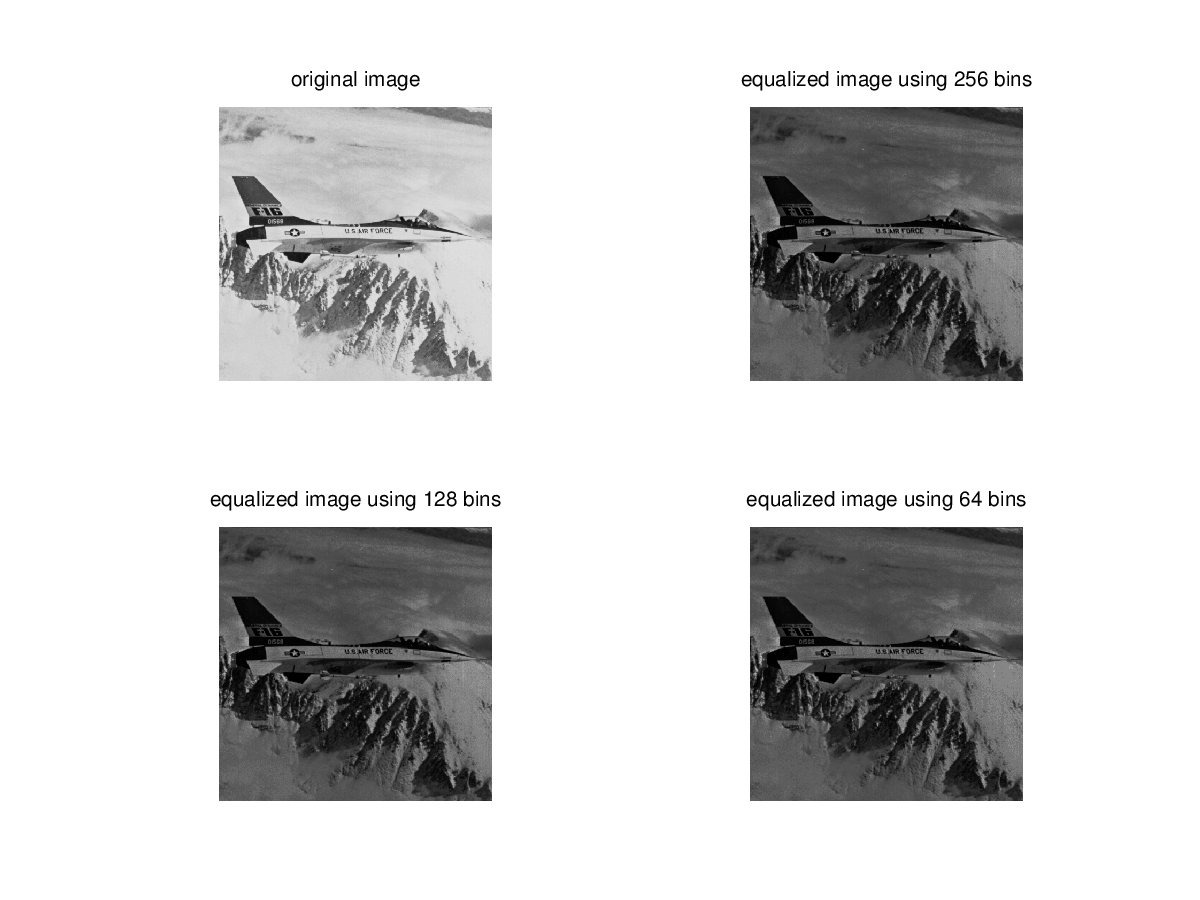
\includegraphics[width=\linewidth]{Q1/outputImages.png}
	\caption{equalized images}
\end{figure}

how to start newpage

\newpage

how to make table

\begin{table}[H]
	\centering
	\begin{tabular}{ c | c | c }
		filter & MSE & PSNR \\
		none & 72.0 & 29.6 \\
		3x3 mean filter & 32.9 & 33.0 \\
		5x5 mean filter & 36.7 & 32.5 \\
		3x3 median filter & 37.2 & 32.4 \\
		5x5 median filter & 36.2 & 32.5 \\
	\end{tabular}
	\caption{SNR and PSNR after filtering the noisy image}
\end{table}
	

\end{comment}
\begin{document}
\maketitle
	\newpage
	\section{Problem 6.16}
	
	\subsection{Part a: Find the missing values of the hue image}
	\begin{figure}[H]
		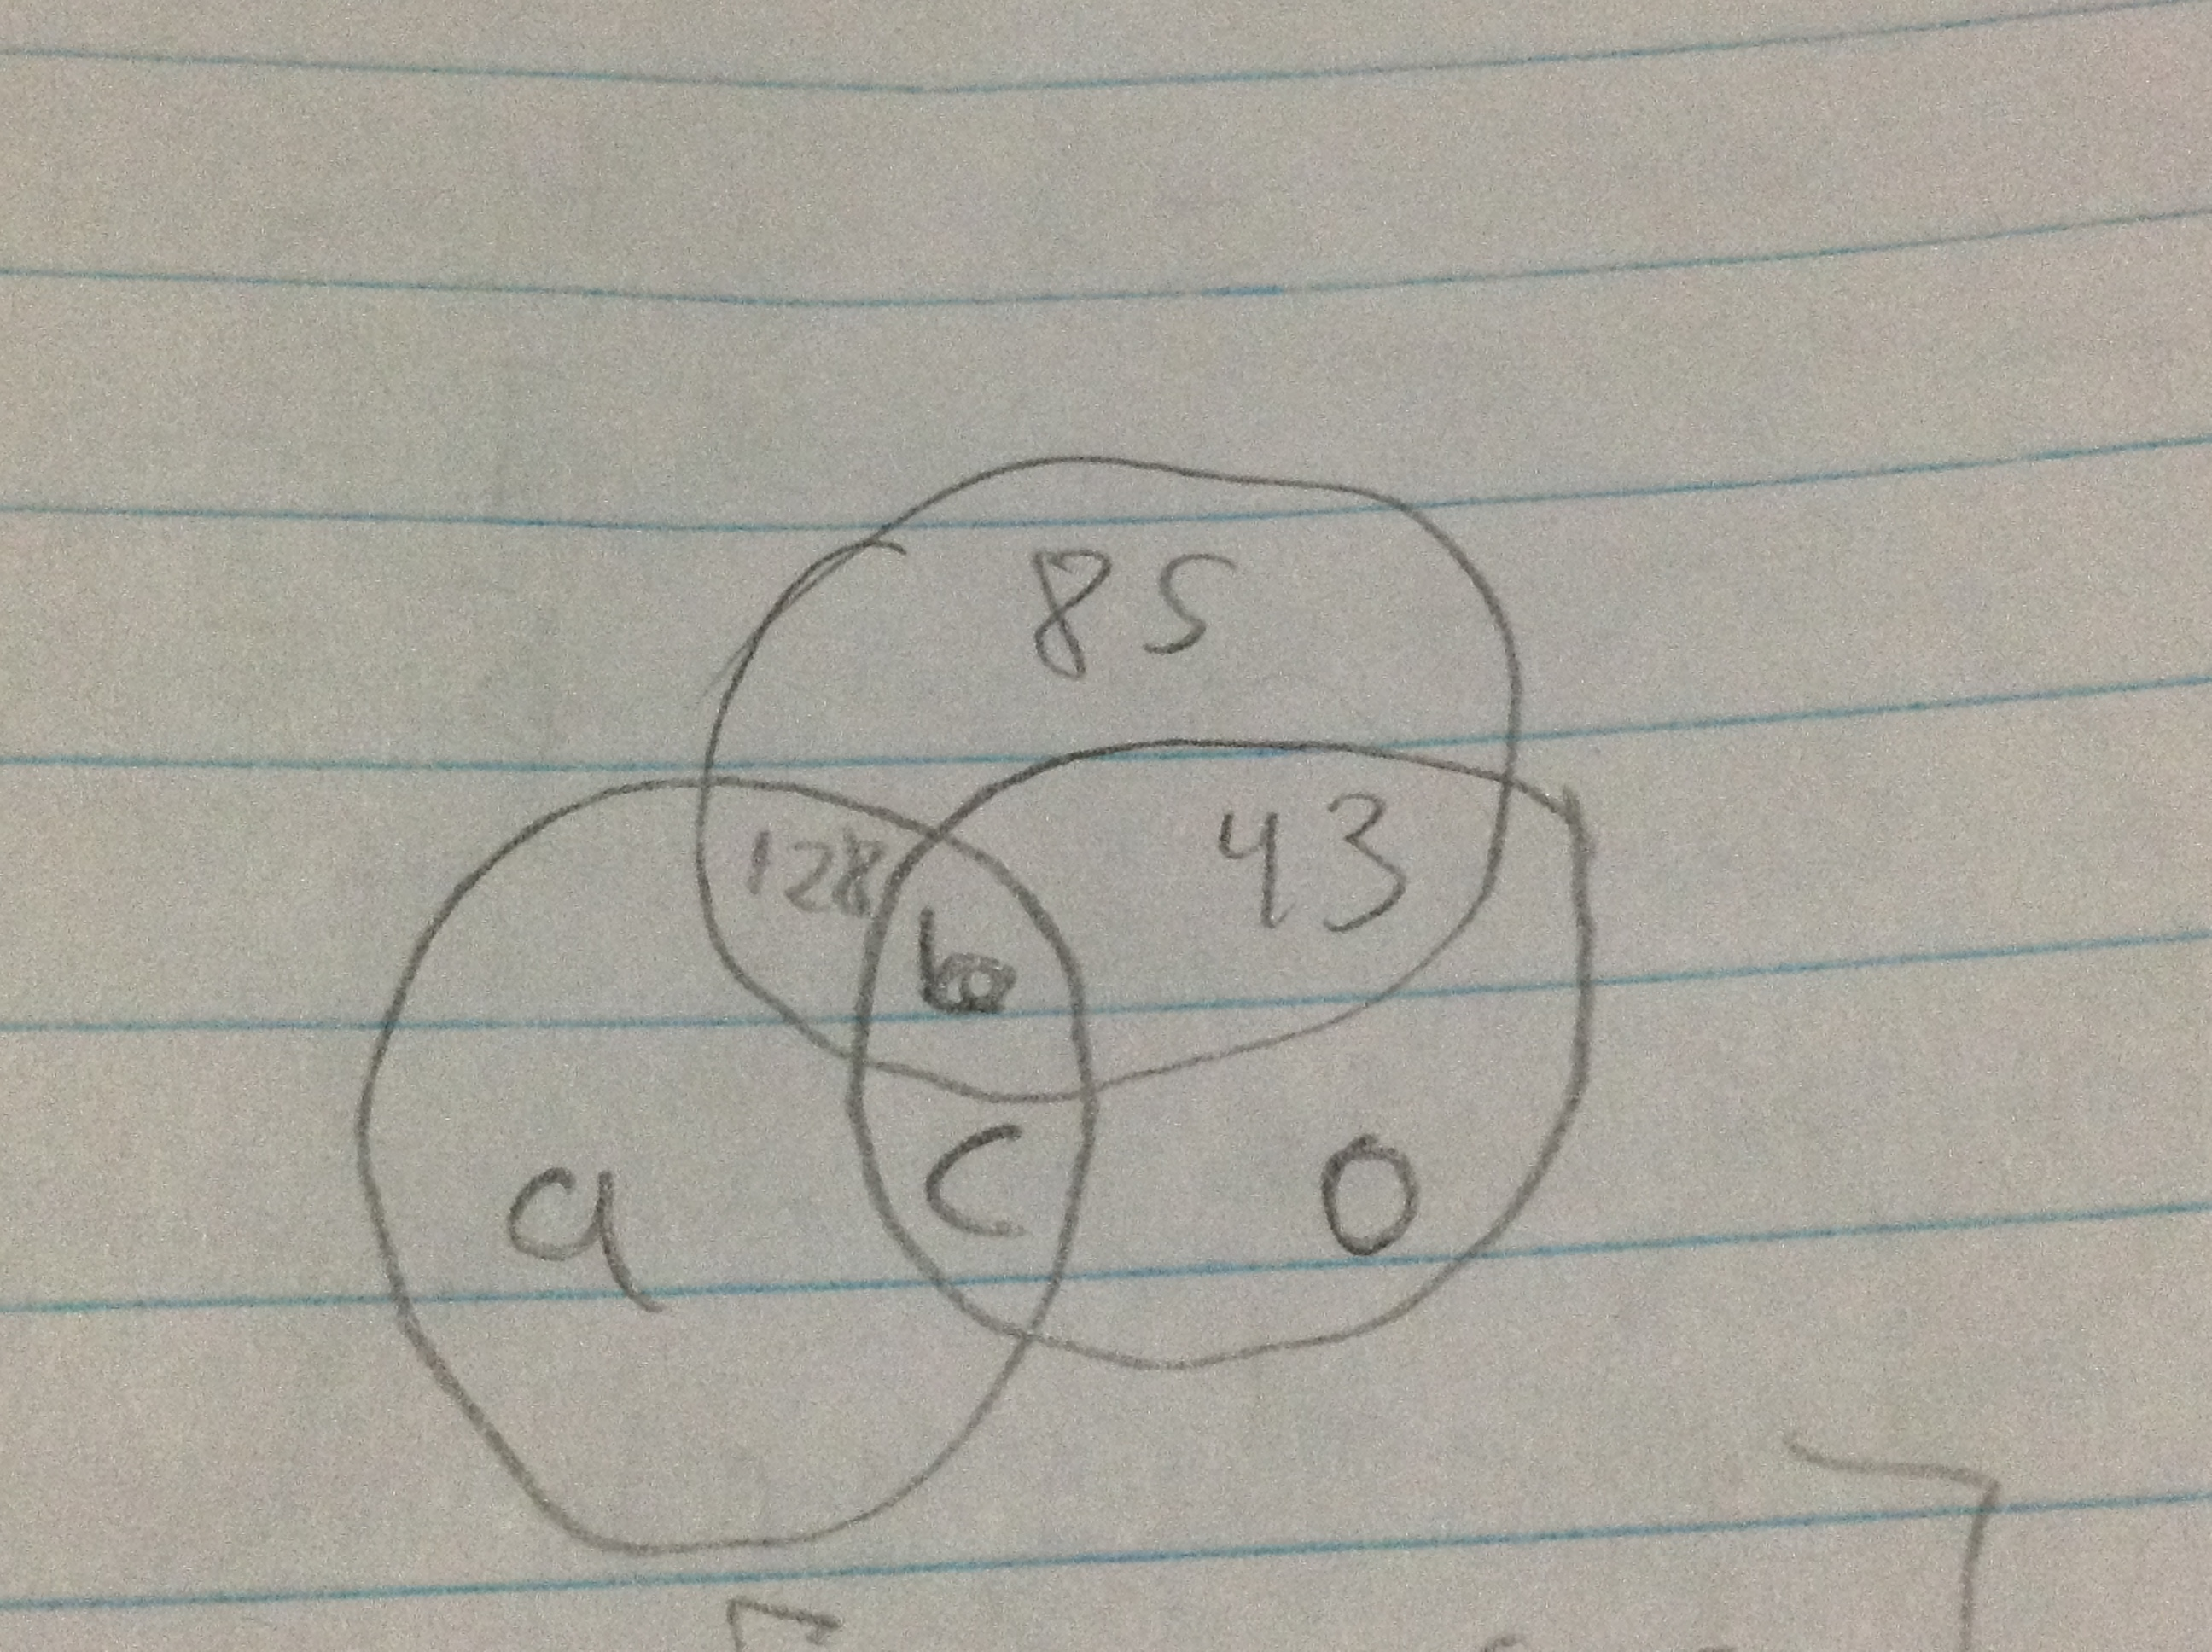
\includegraphics[width=\linewidth]{6.16/fig1.JPG}
		\caption{H image pixel values a, b, and c are missing}
	\end{figure}
	
	We can convert the pixel values to hue values using the following equation.
	\[(pixel)\frac{360}{255} = hue\]
	We are given the following pixel values: 0, 43, 85, and 128.
	Using the formula we obtain the following hue values: 0, 60, 120, and 180.
	Looking at the hue color wheel, we get the following colors: red(0), yellow(60), green(120), and cyan(180).
	Since the overlap between red(0) and green(120) results in yellow(60), we can infer the colors a, b, and c. The addition of a and green(120) give cyan(180). This implies that a is blue(240). The addition of blue(240) and red(0) give c, which is magenta(300). The addition of red(0), blue(240), and green(120) gives b, which is white(0).
	We can convert the hue values to pixel values using the following equation.
	
	\[(hue)\frac{255}{360} = pixel\]
	
	Using this formula we can get the missing pixel values: b(0), a(170), and c(212).
	We can assume the background is black, since color addition works.
	
	\begin{figure}[H]
		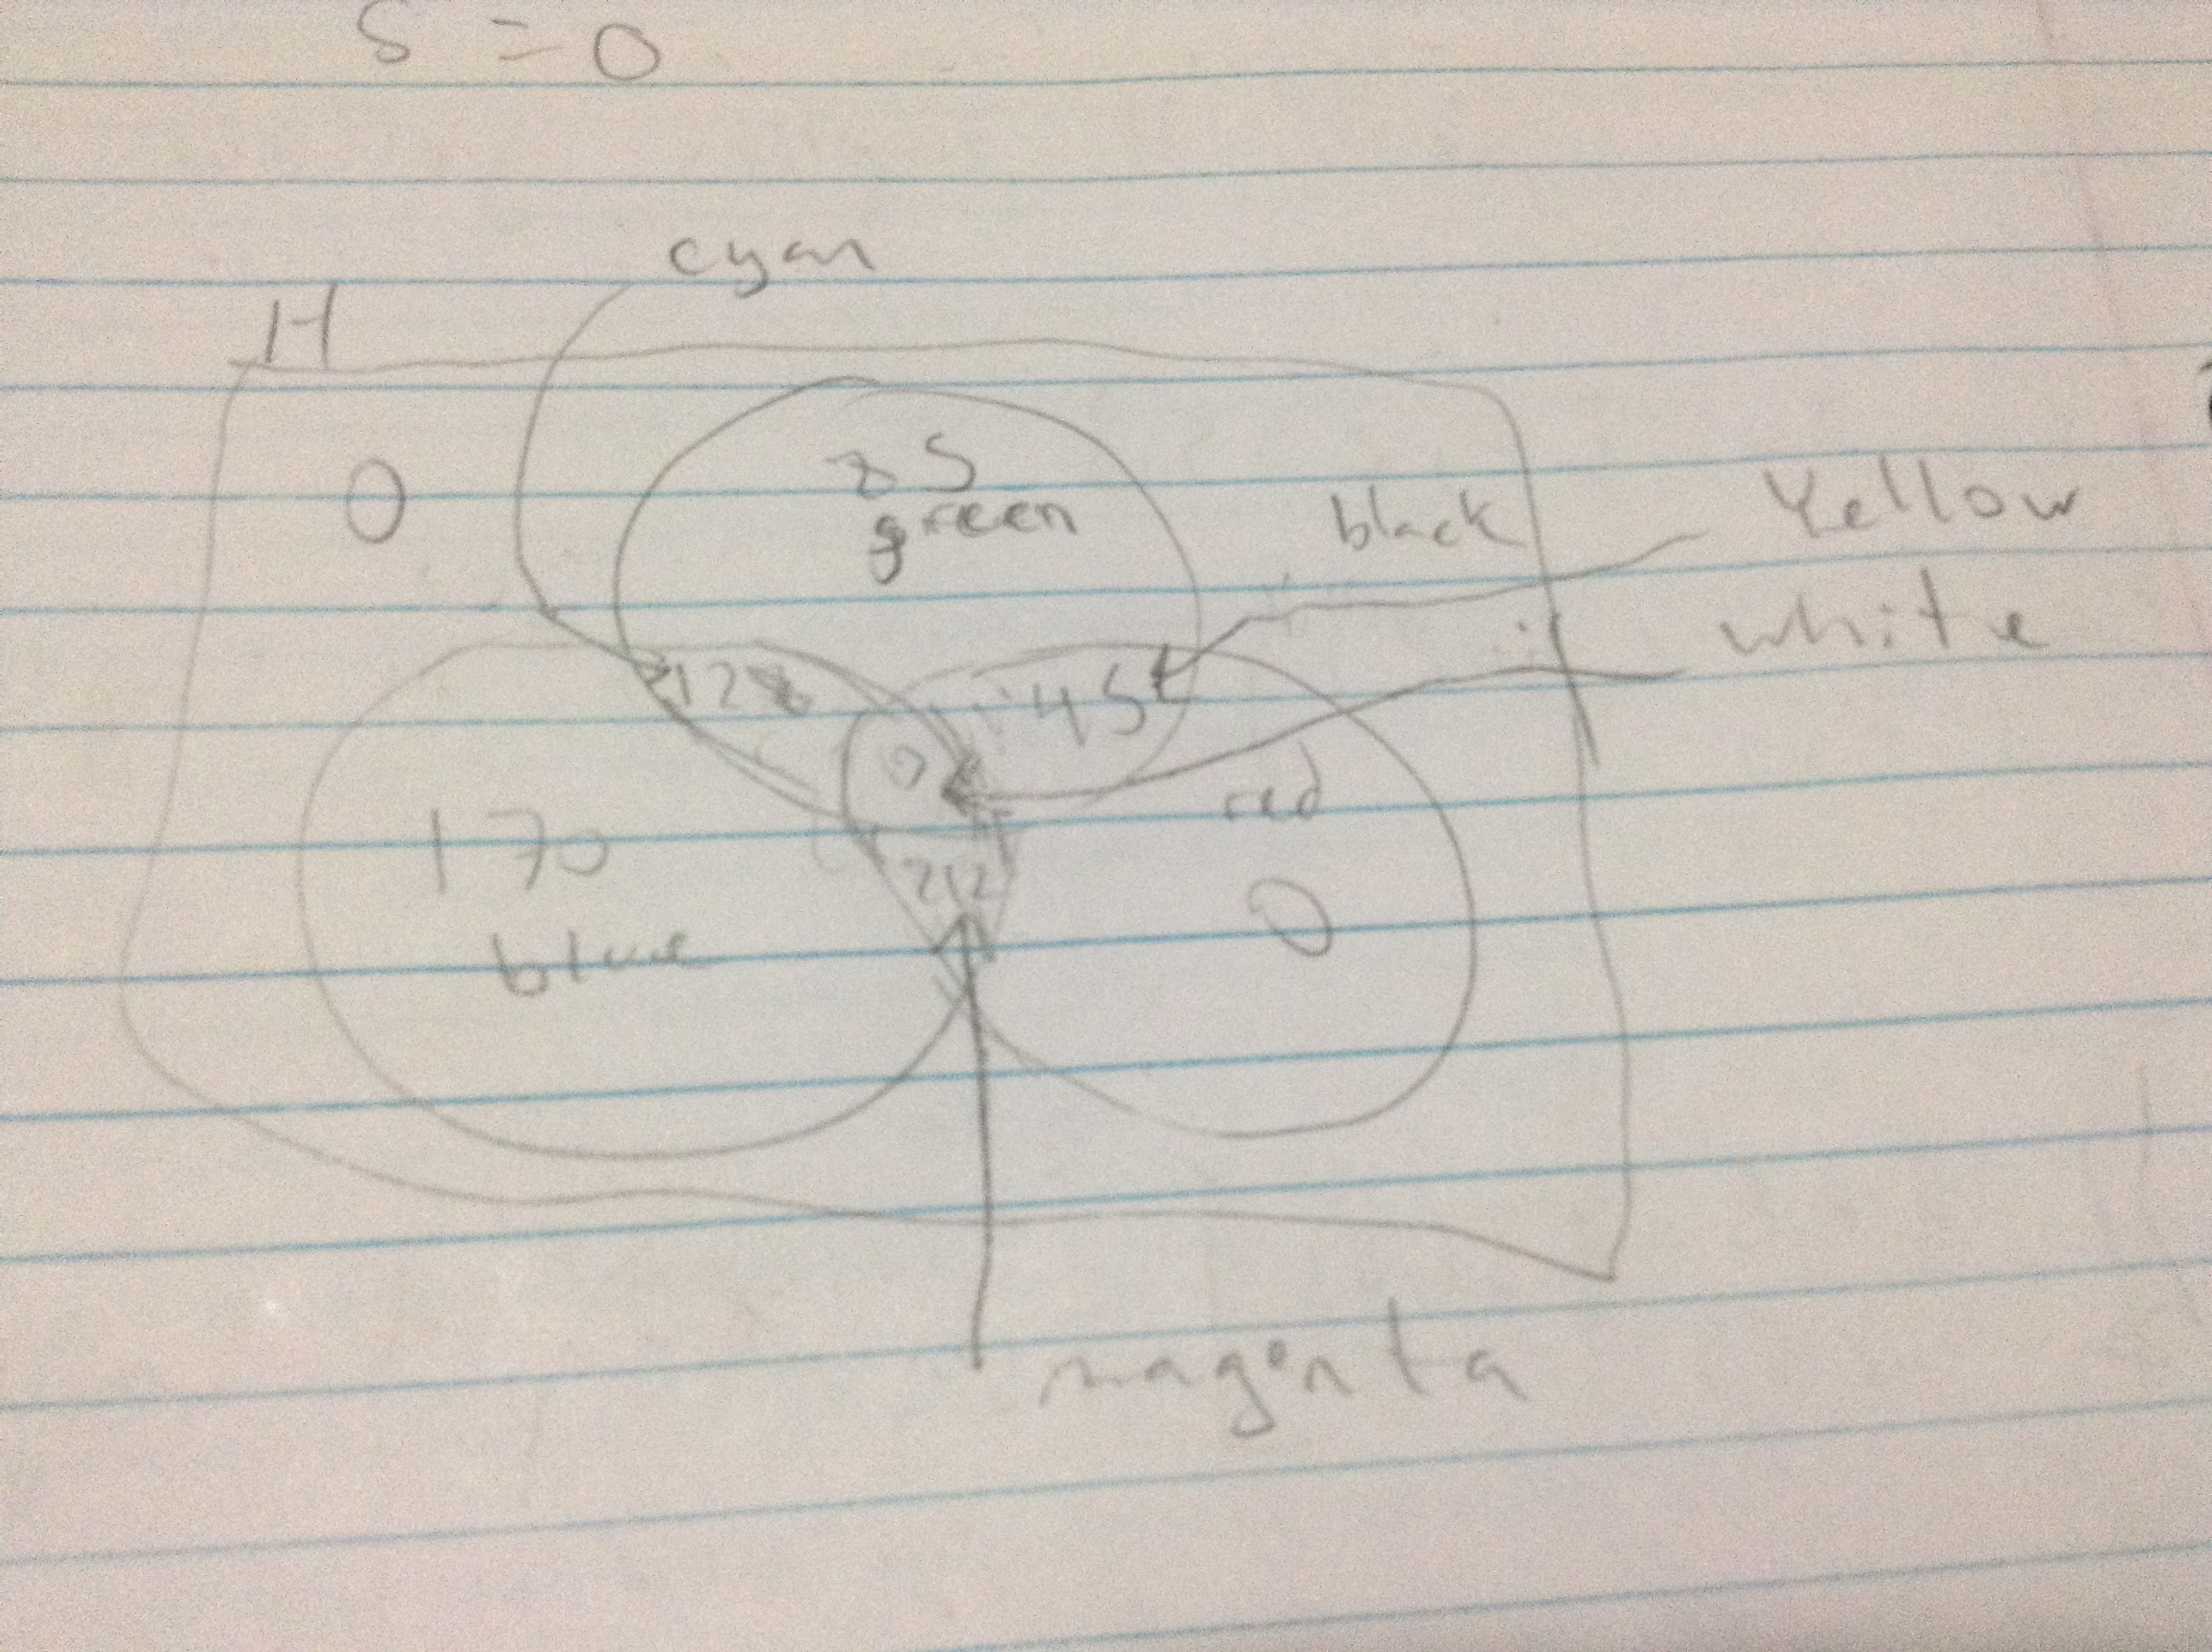
\includegraphics[width=\linewidth]{6.16/fig2.JPG}
		\caption{H image pixel values a, b, and c are missing}
	\end{figure}
	
	\subsection{Part b: Find the missing values of the saturation image}
	
	\begin{figure}[H]
		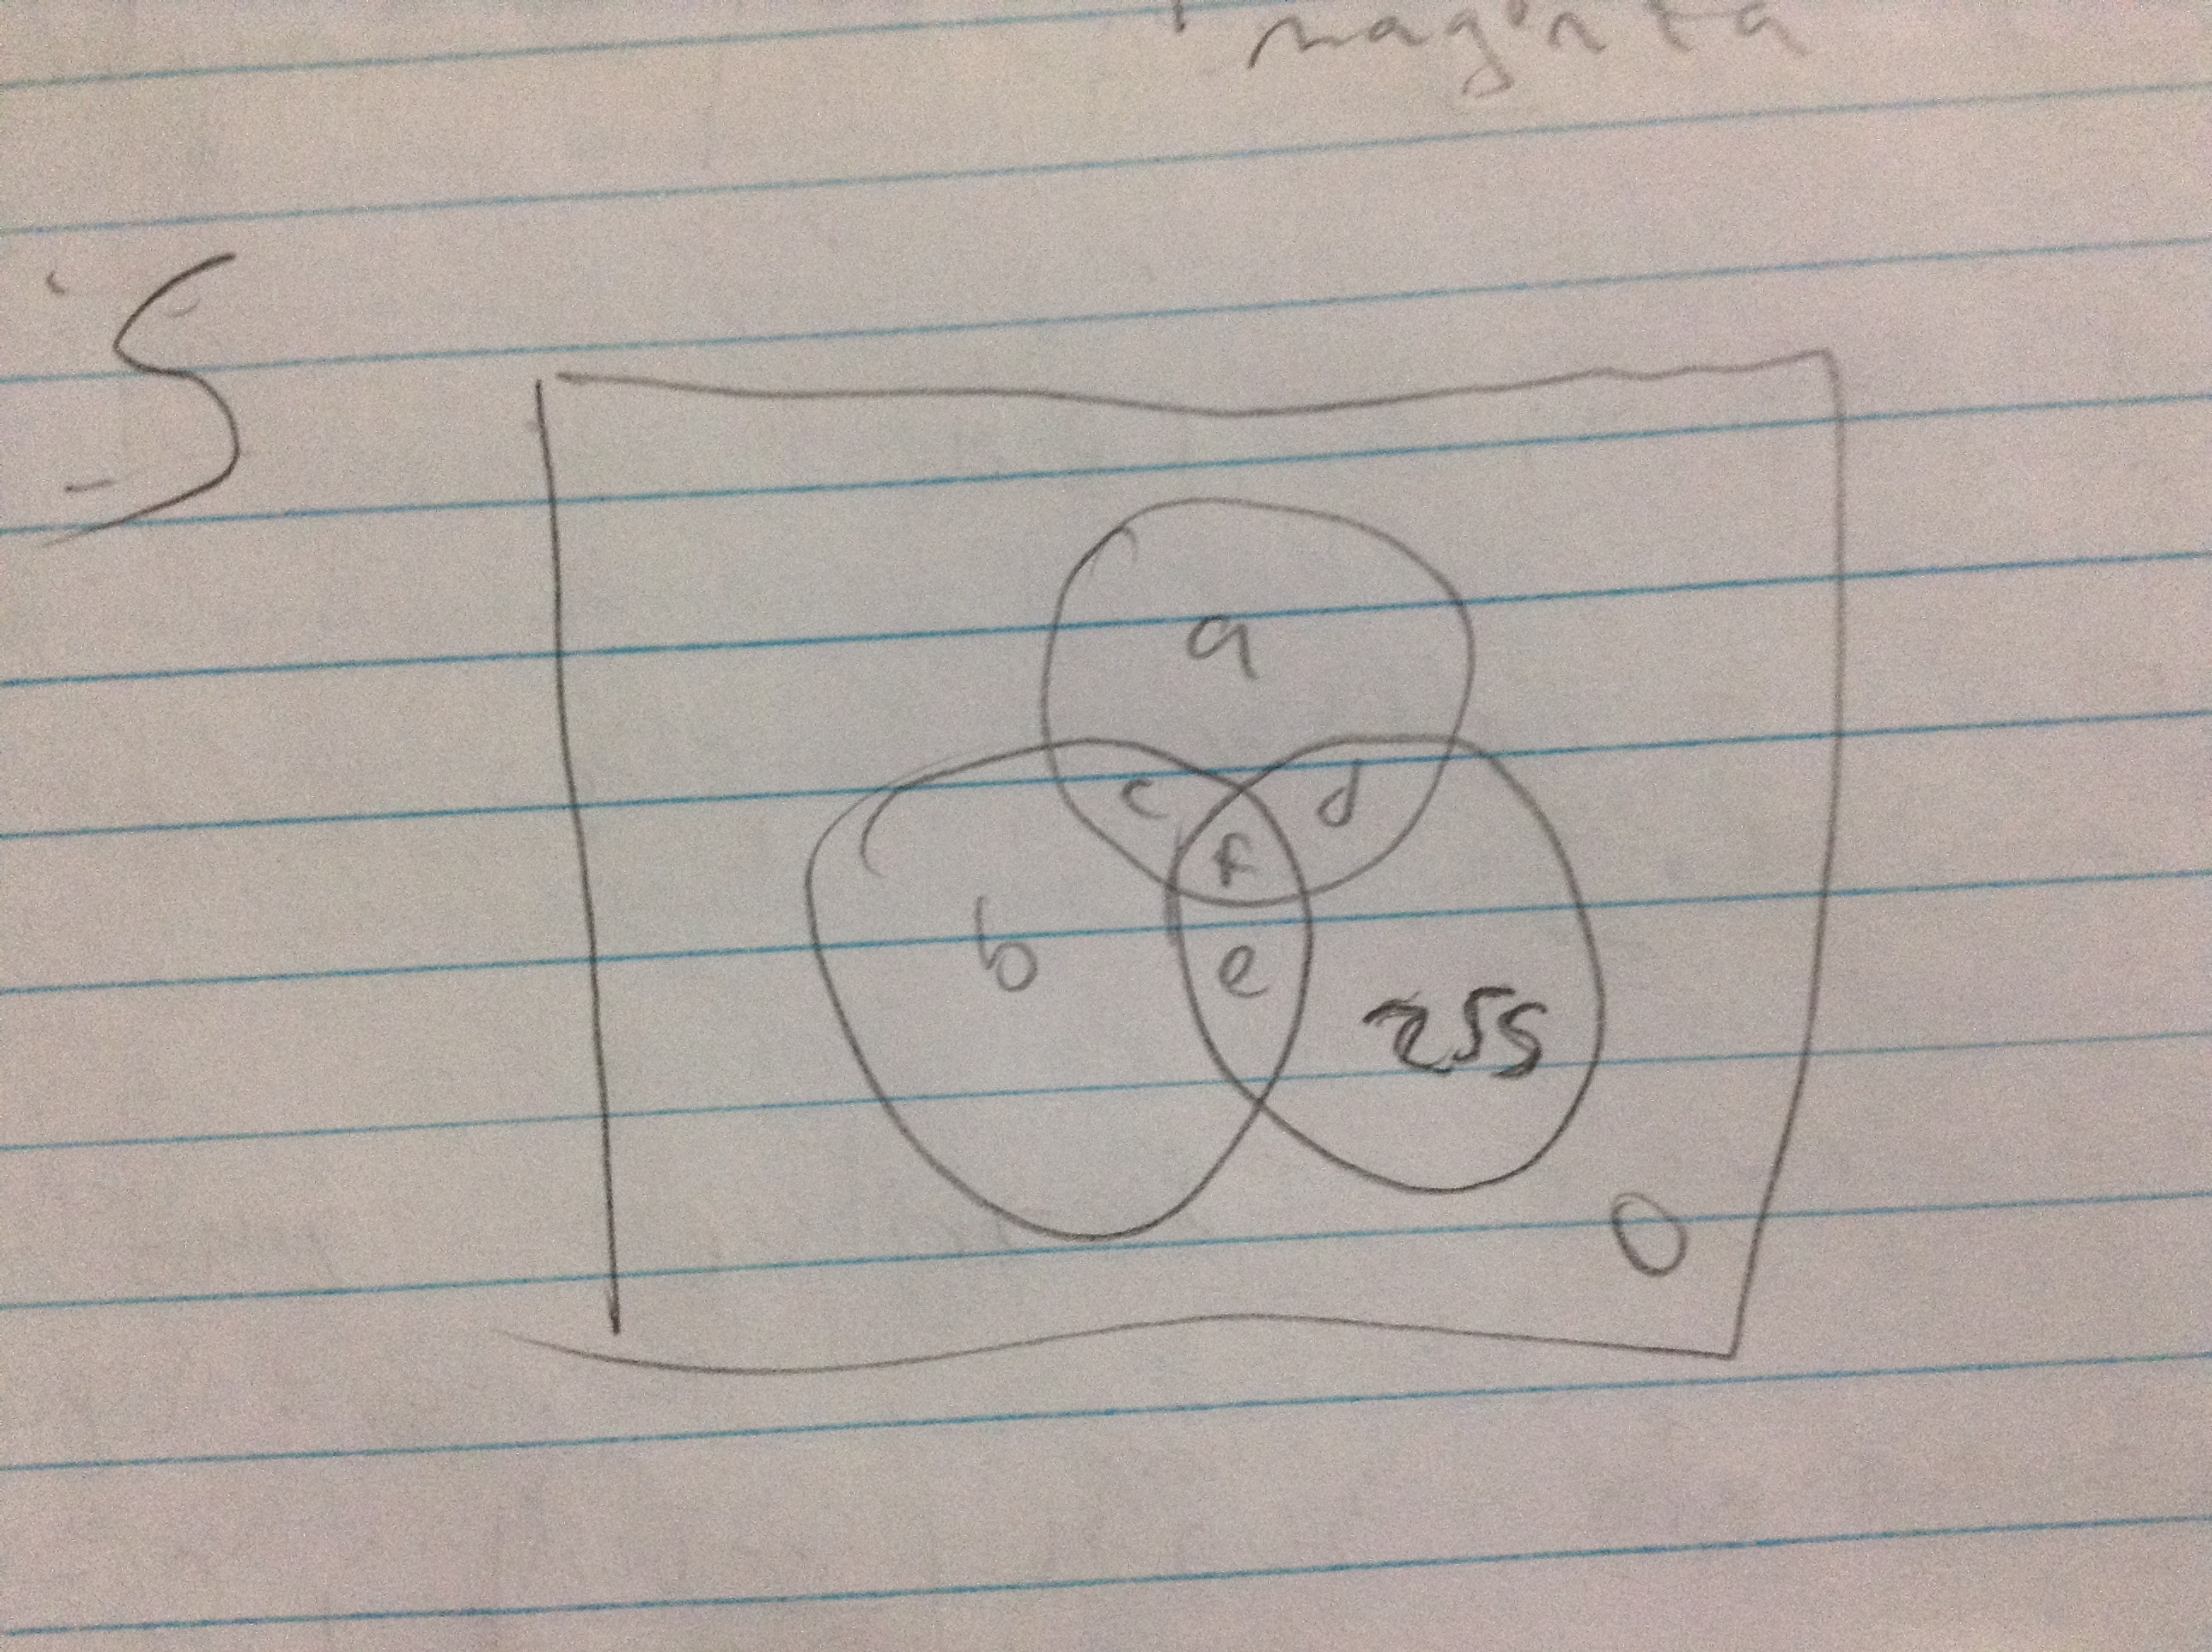
\includegraphics[width=\linewidth]{6.16/fig3.JPG}
		\caption{S image pixel values}
	\end{figure}
	
	We can infer that all of the colors have the same saturation, since we were able to add them together in part a. Red has a saturation of 255, so all of the remaining colors must also have this level of saturation. The white part is the only different one, since white has zero saturation in HSI space as it corresponds to a point.
	
	\begin{figure}[H]
		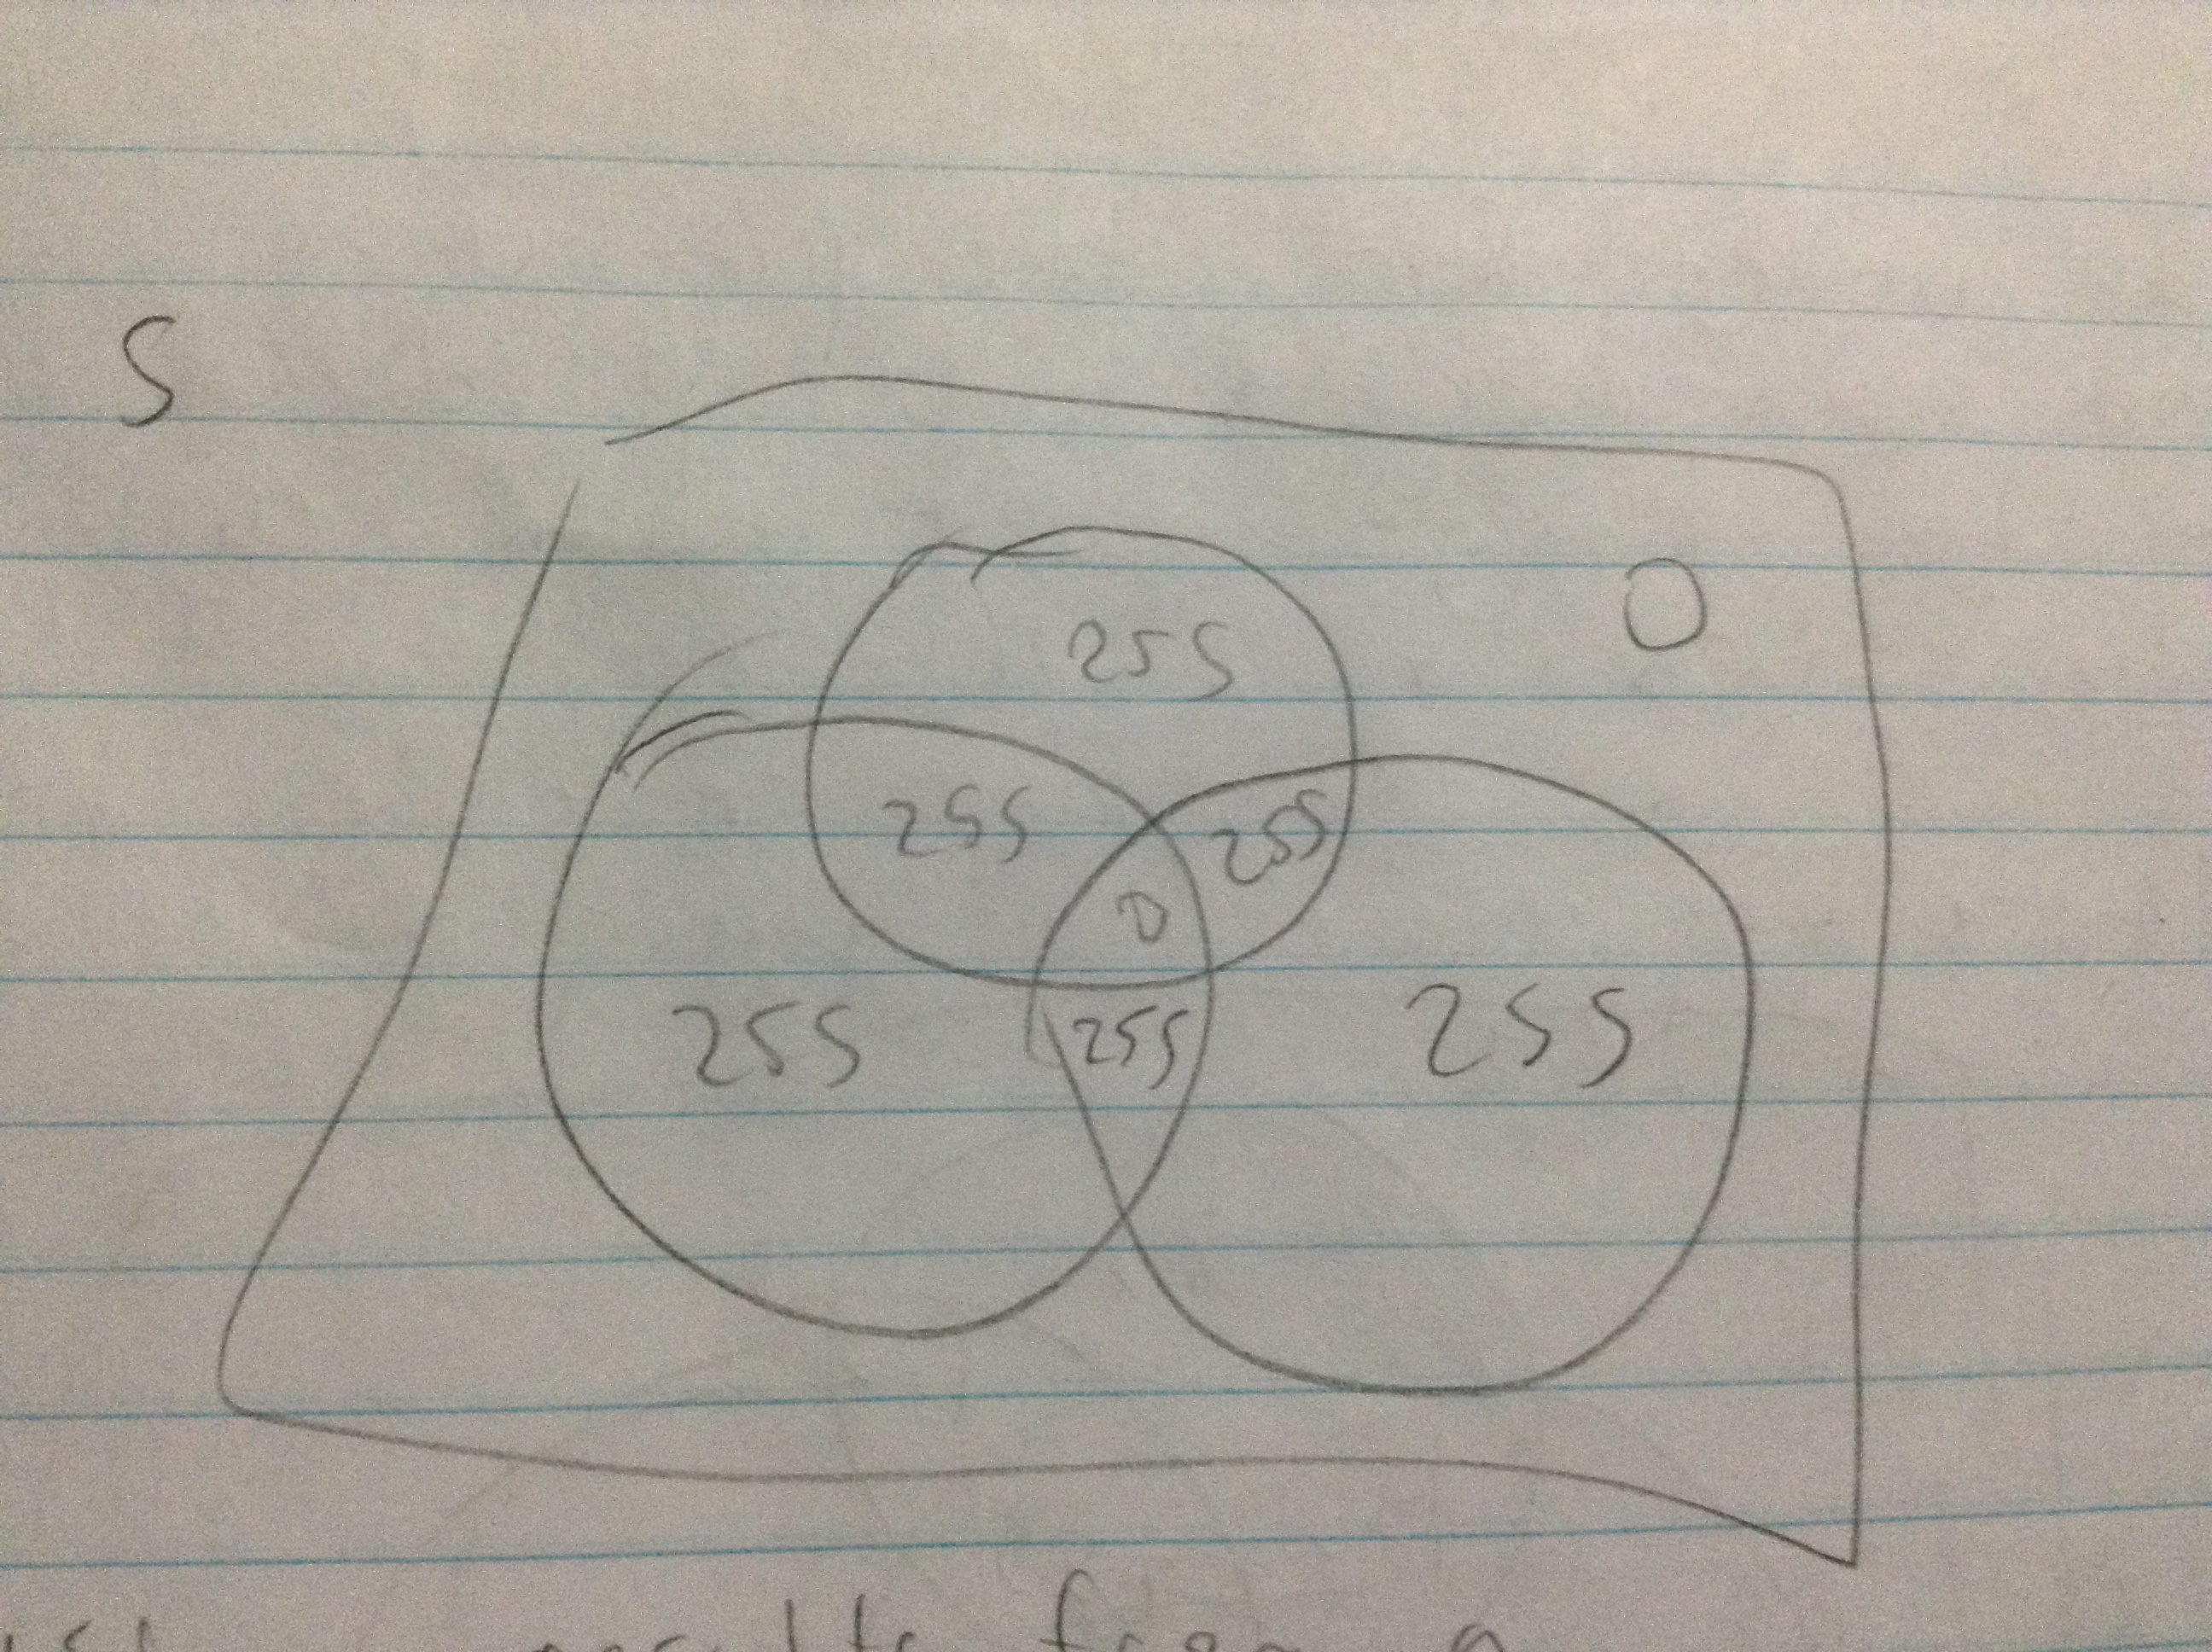
\includegraphics[width=\linewidth]{6.16/fig4.JPG}
		\caption{S image pixel values}
	\end{figure}
	
	\subsection{Part c: Find the missing values of the intensity image}
	
	\begin{figure}[H]
		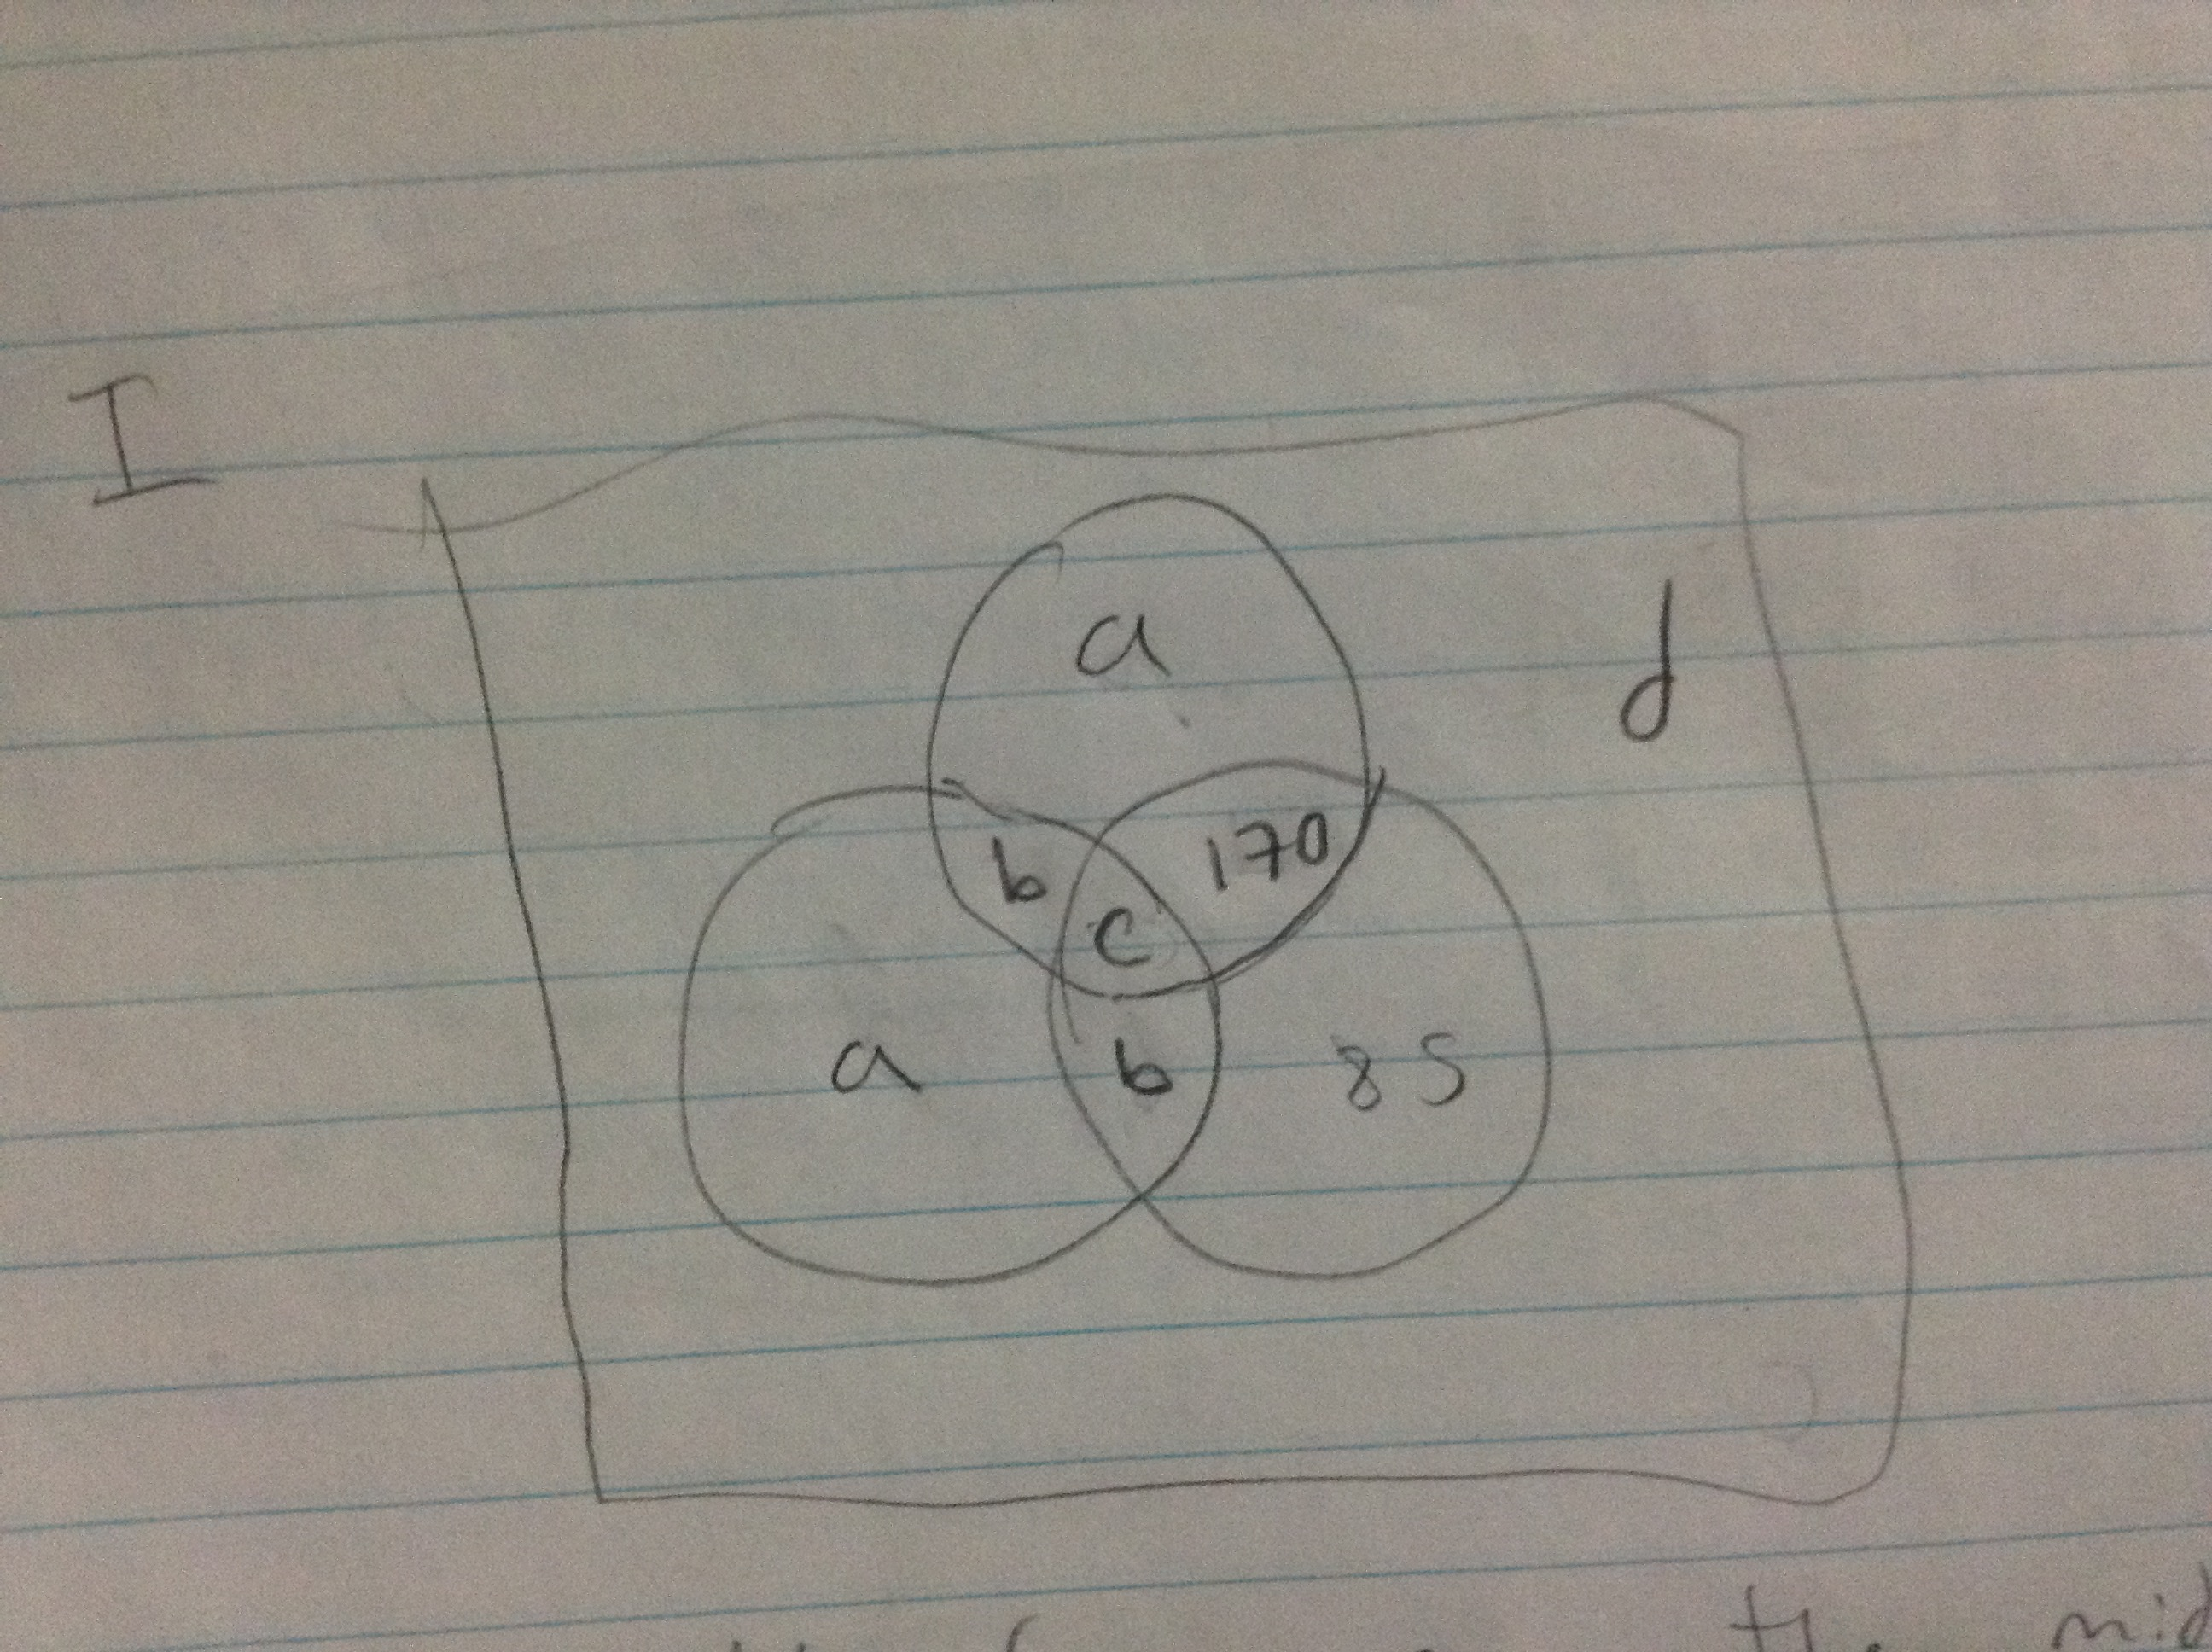
\includegraphics[width=\linewidth]{6.16/fig5.JPG}
		\caption{I image pixel values}
	\end{figure}
	
	We are given the intensity values for red (85) and yellow (170). Using the results from part a, we can infer the values of c and d since they correspond to black and white. C must be equal to 255, white has max intensity. D must be equal to 0, black has zero intensity. The fact that red, green, and blue turn into white implies that they have equal intensity. This also applies to cyan, yellow, and magenta. Thus, a must equal 85 and b must equal 170.
	
	\begin{figure}[H]
		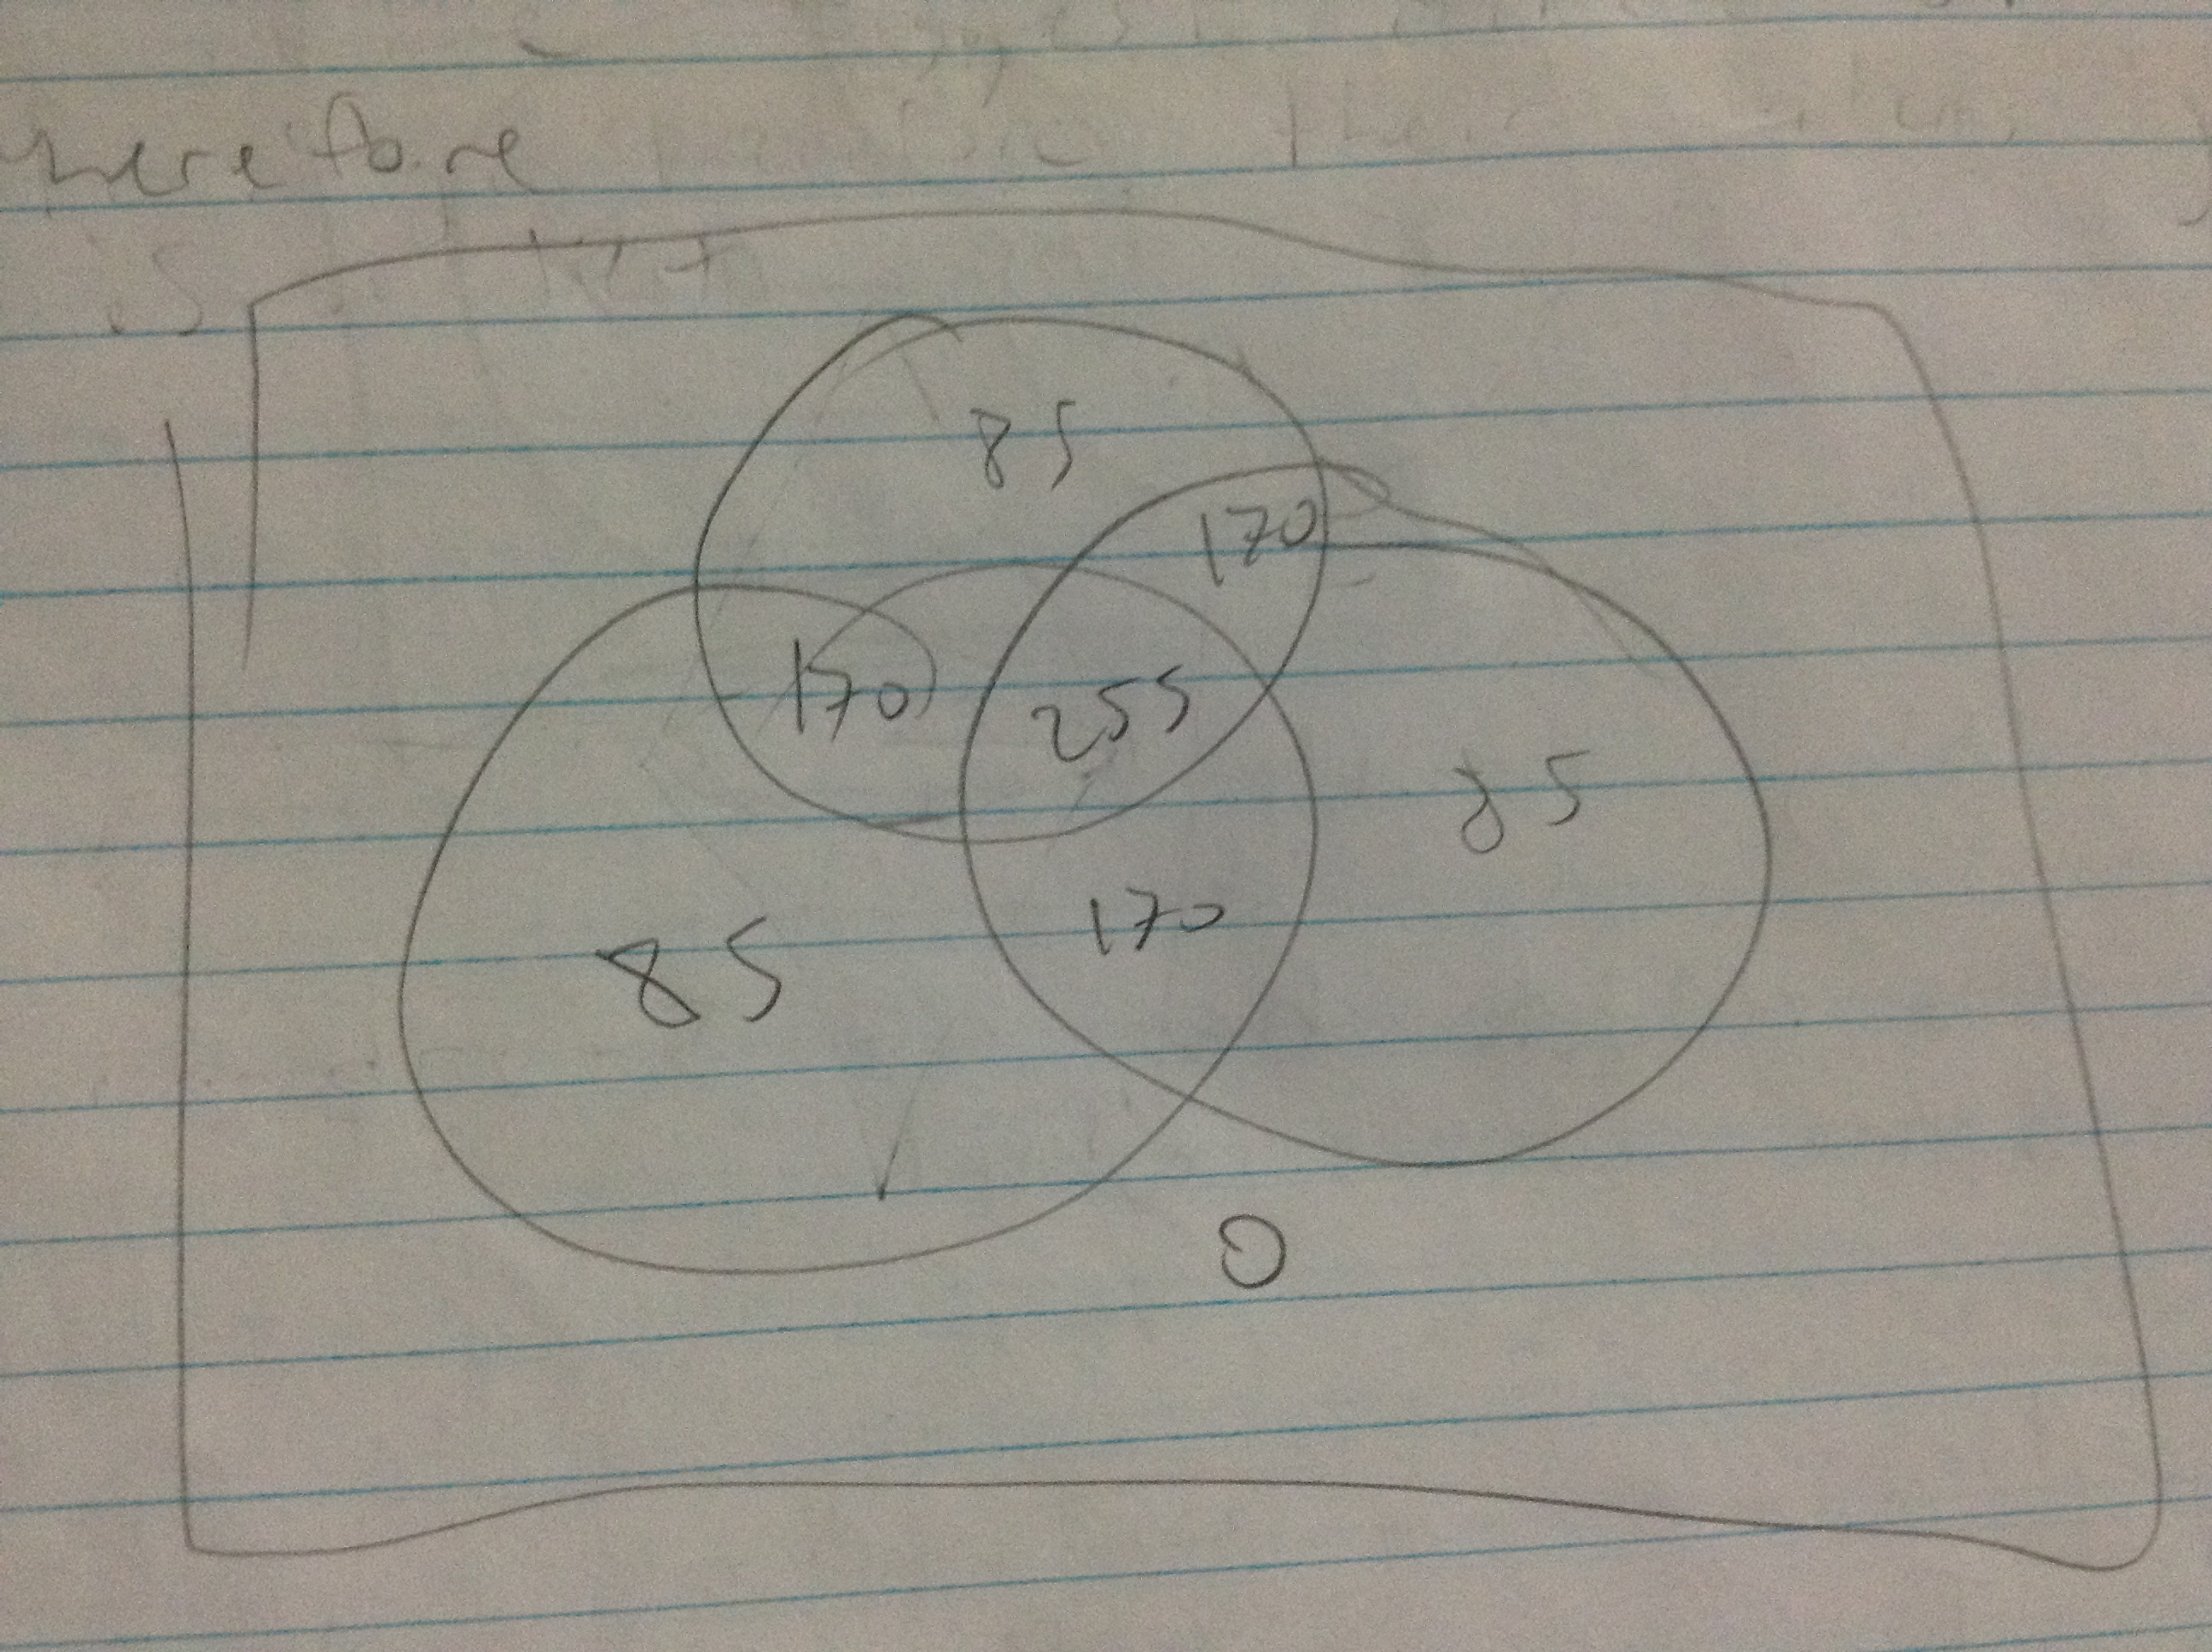
\includegraphics[width=\linewidth]{6.16/fig6.JPG}
		\caption{I image pixel values}
	\end{figure}
	
	\newpage
	\section{Problem 6.17}
	
	\subsection{Part a: Why is the image mostly red?}
	
	\begin{figure}[H]
		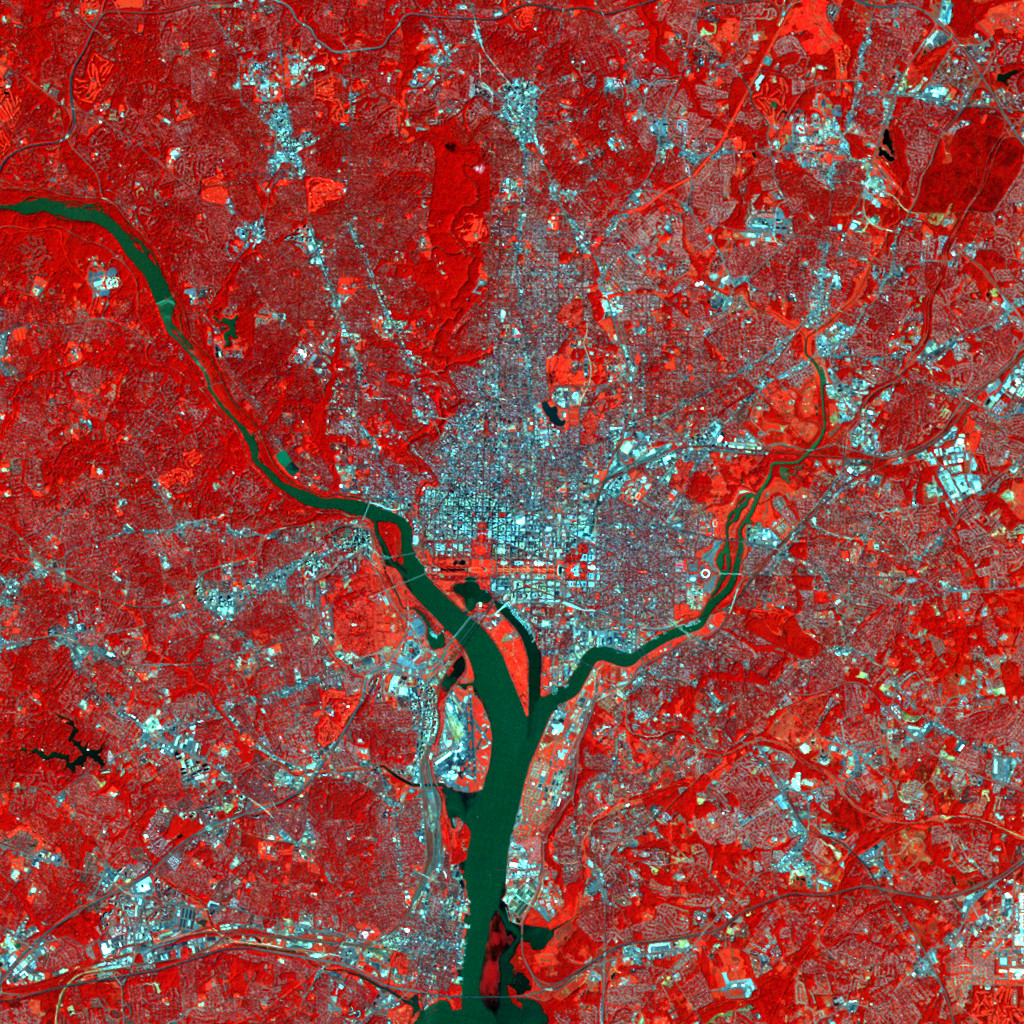
\includegraphics[width=\linewidth]{6.17/partA/washingtonDCREDinfra.png}
		\caption{modified image of Washington DC}
	\end{figure}
	
	This image is a modified version of an aerial photo of Washington DC.
	
	\begin{figure}[H]
		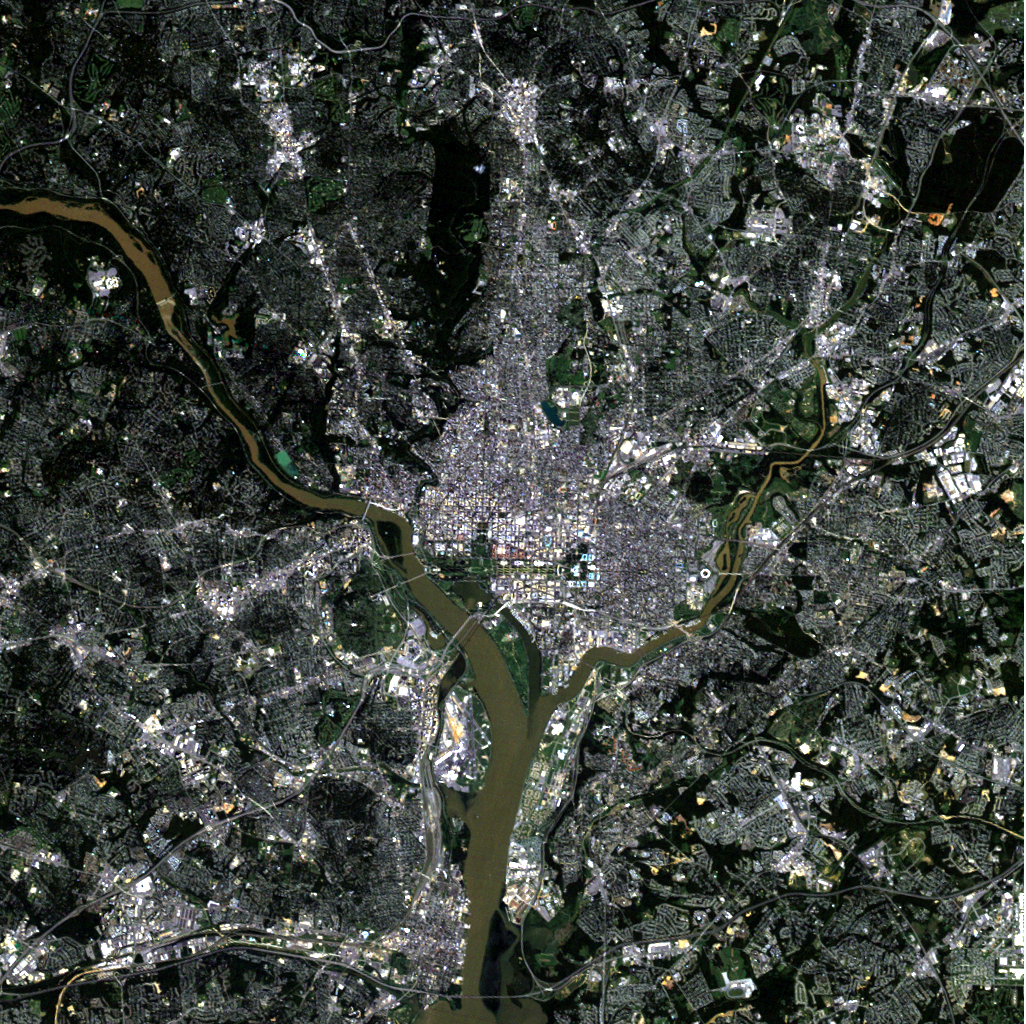
\includegraphics[width=\linewidth]{6.17/partA/washingtonDCcolor.png}
		\caption{original image of Washington DC}
	\end{figure}
	
	The modified image was produced by using the pixel values of an infrared image instead of the original values of the red channel. Since the infrared image has higher values corresponding to vegetation and terrain, the modified image shows the terrain as red.
	
	\begin{figure}[H]
		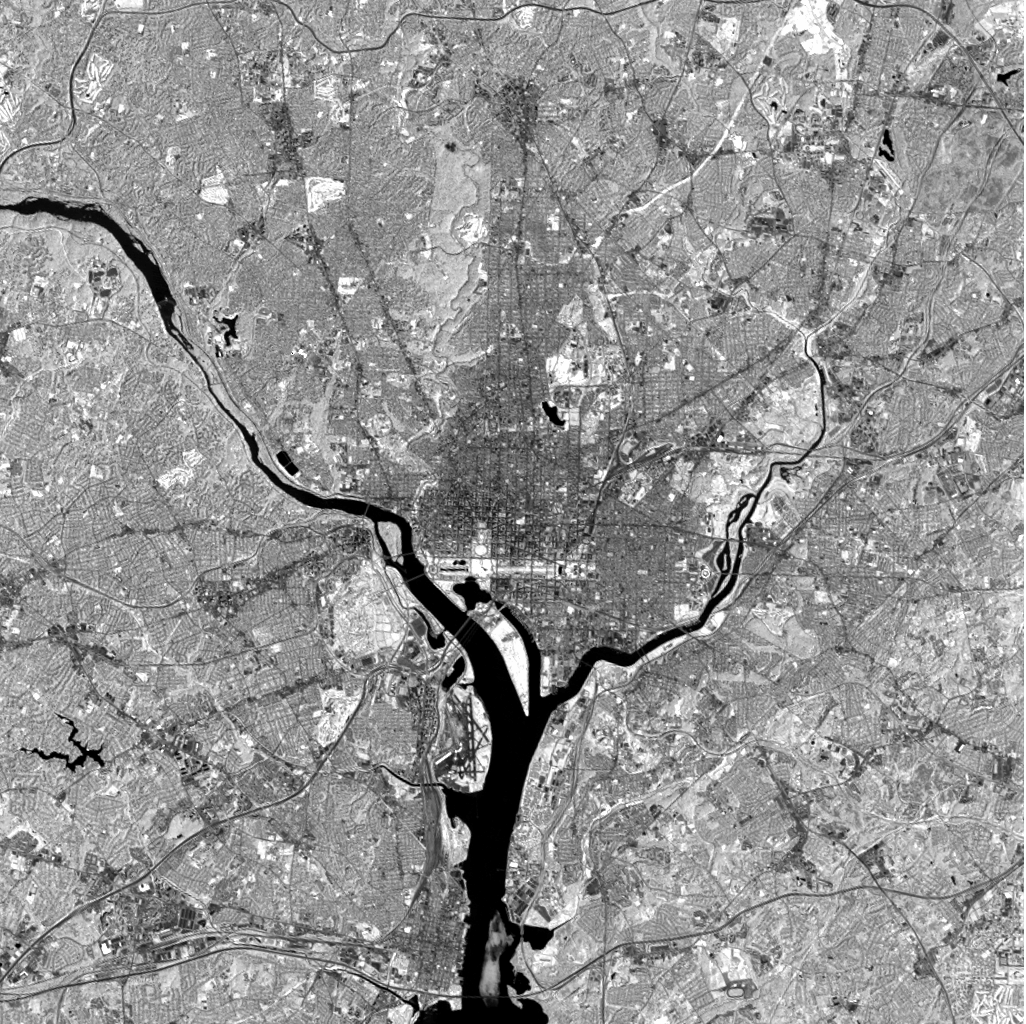
\includegraphics[width=\linewidth]{6.17/partA/infra.png}
		\caption{infrared gray-scale image of Washington DC}
	\end{figure}
	
	\subsection{Part b: Write a procedure for coloring the water blue}
	Looking at the infrared image, we can see that water has very low pixel values. We can threshold the infrared image to produce a mask that only contains water.
	\begin{figure}[H]
		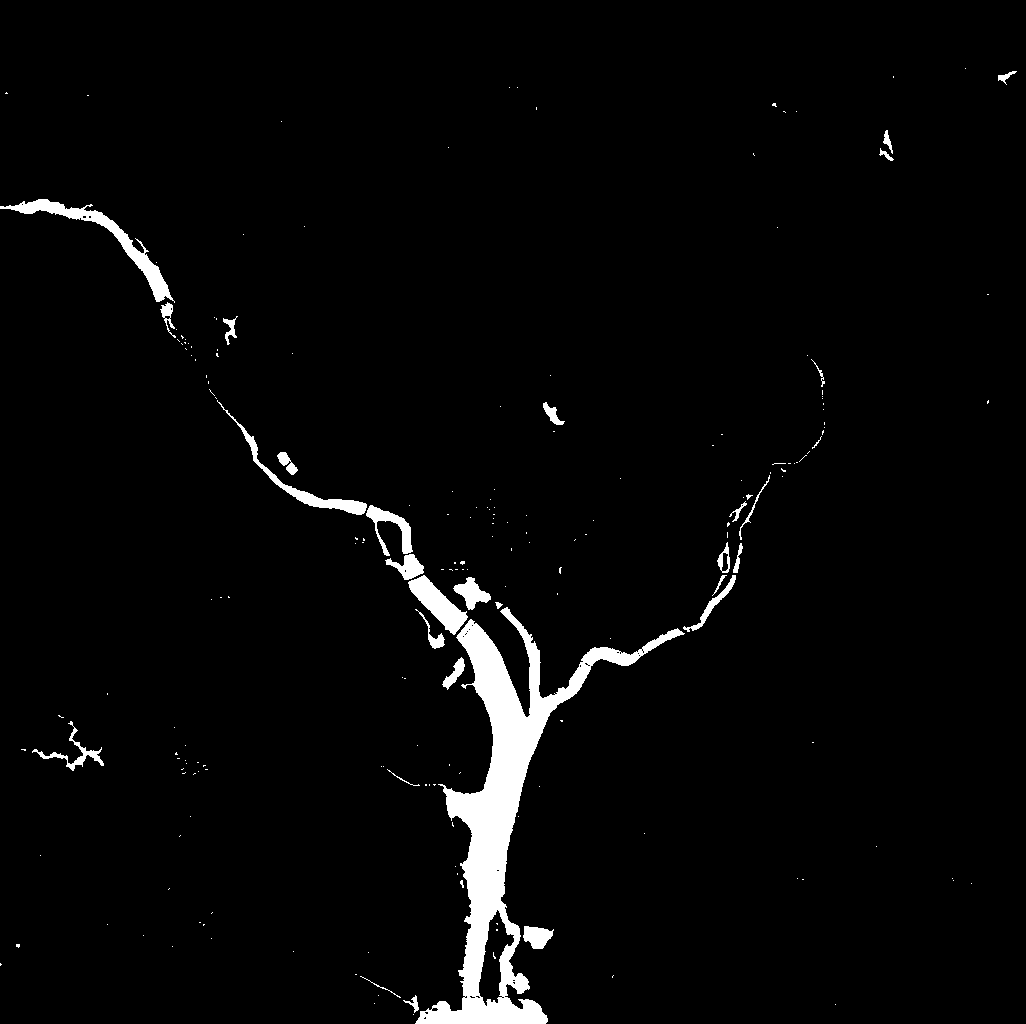
\includegraphics[width=\linewidth]{6.17/partB/water.png}
		\caption{water mask}
	\end{figure}
	We can then add our mask to the blue channel to accentuate the water in the color image.
	\begin{figure}[H]
		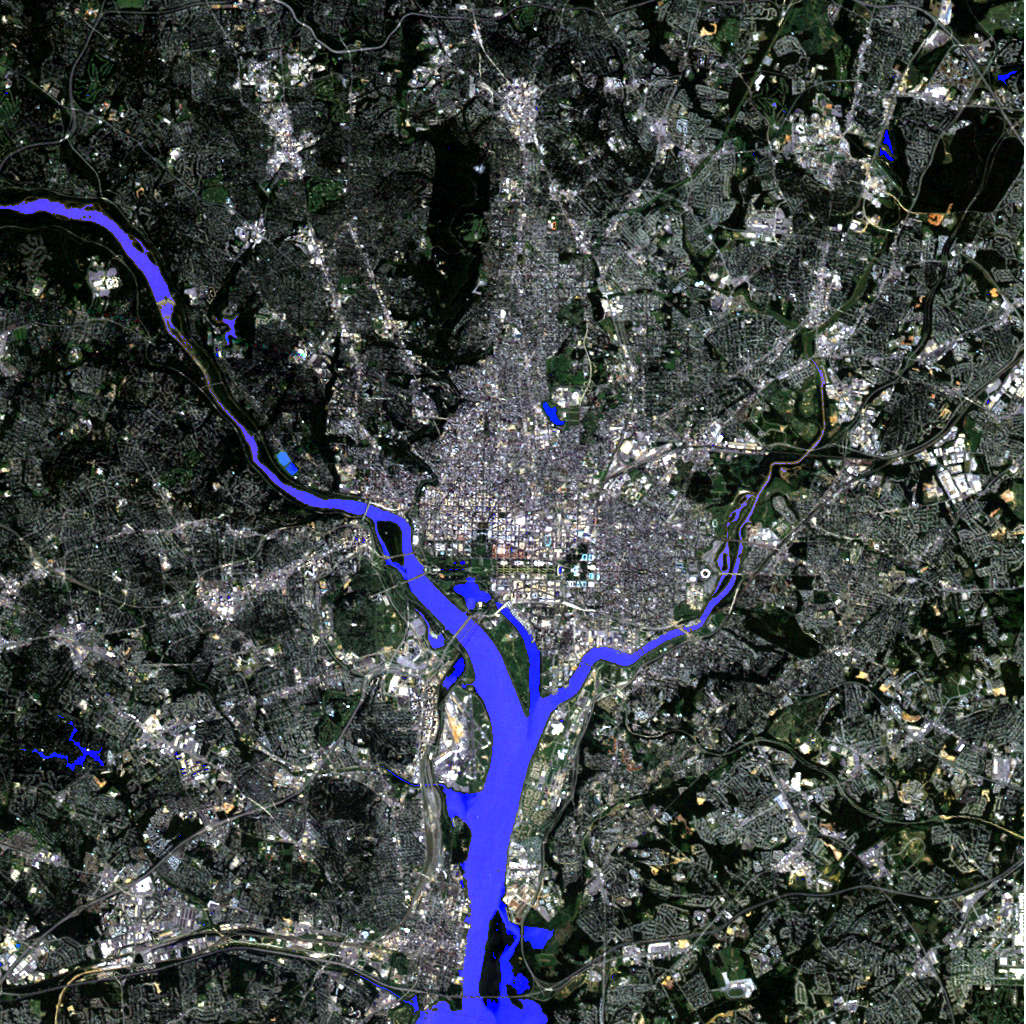
\includegraphics[width=\linewidth]{6.17/partB/washingtonDCwater.png}
		\caption{image of Washington DC with mask added to blue channel}
	\end{figure}
	
	\subsection{Part c: Write a procedure for coloring the man made objects red}
	Looking at the color image we can see that man made objects in the color image look lighter, most being gray or white. The terrain is very dark (black and dark green). Using these observations we can threshold the color channels to generate a mask that shows only man made objects.
	\begin{figure}[H]
		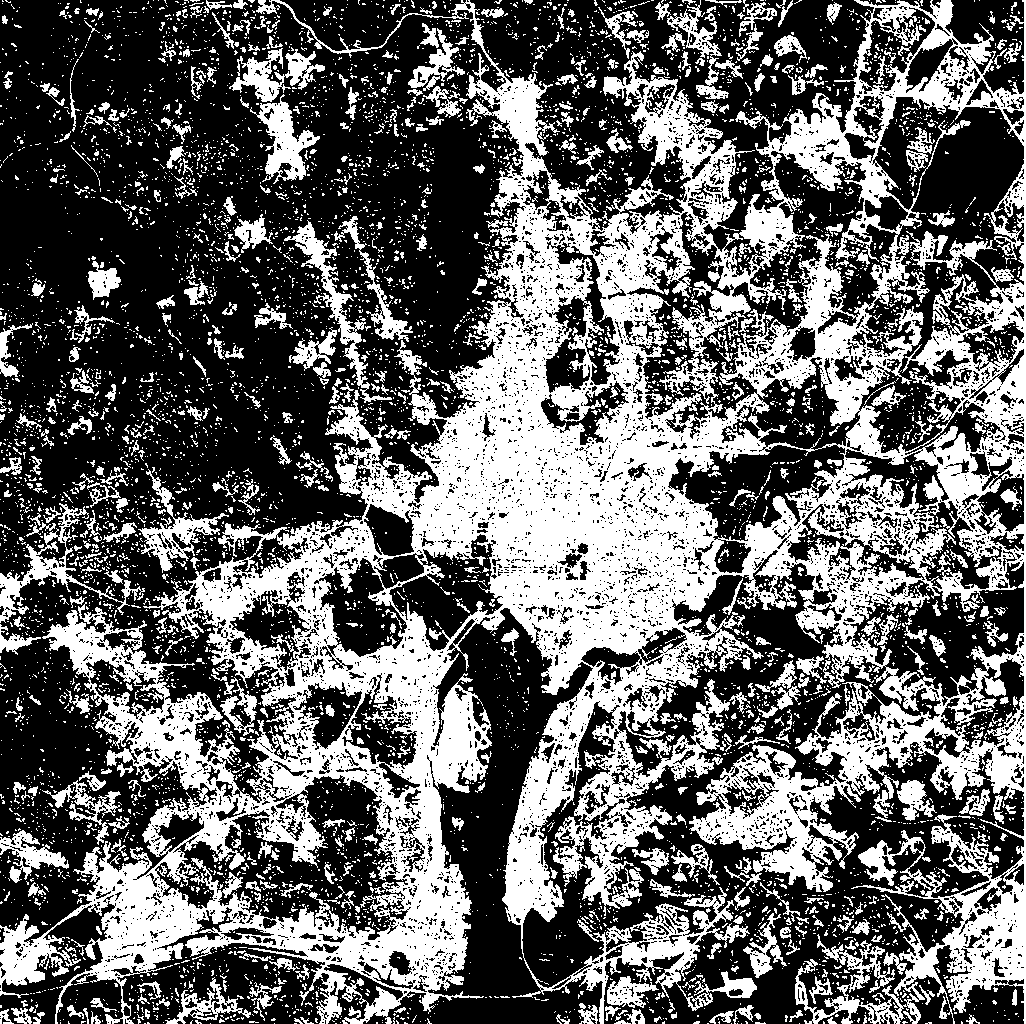
\includegraphics[width=\linewidth]{6.17/partC/buildings.png}
		\caption{man made object mask}
	\end{figure}
	We can then add our mask to the red channel and subtract it from the other channels to accentuate the man made structures in the color image. We subtract from the green and blue channels, because many of the man made structures are white (their red values are already high).
	\begin{figure}[H]
		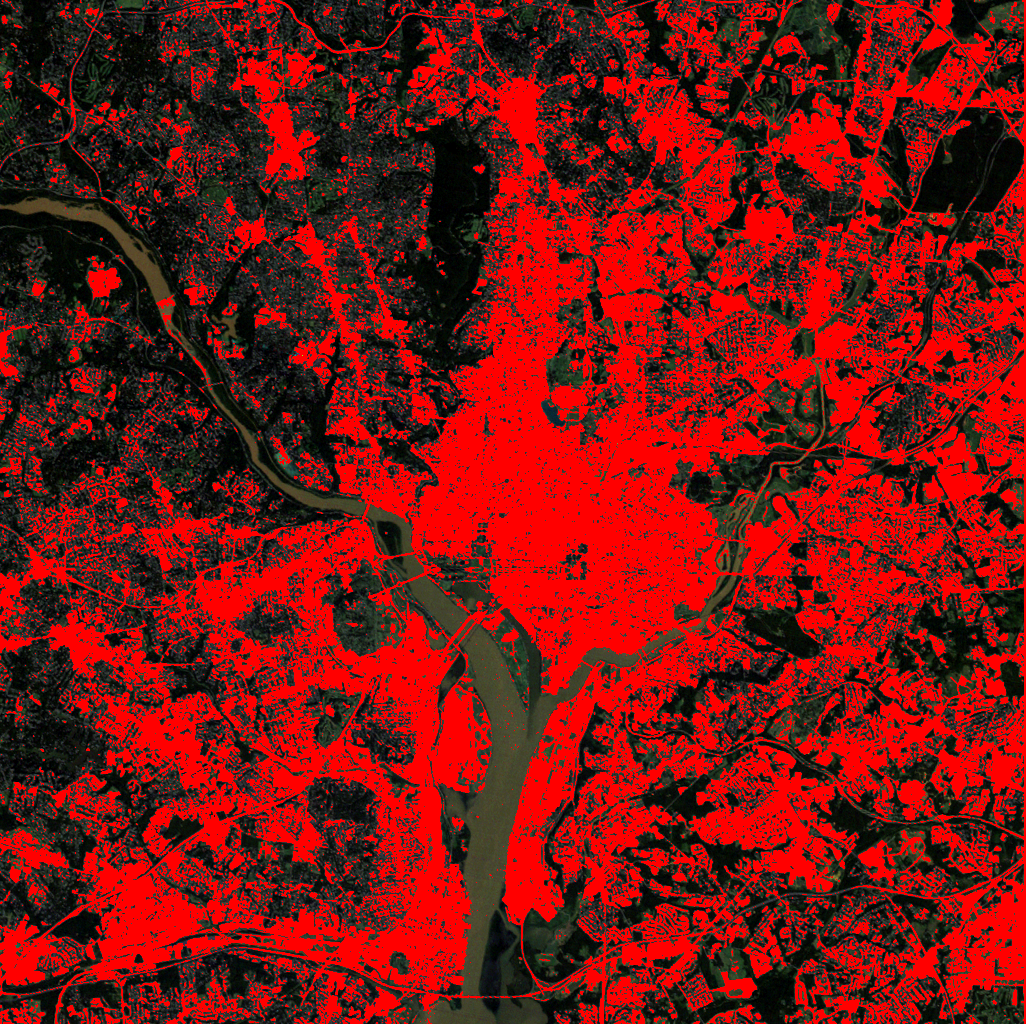
\includegraphics[width=\linewidth]{6.17/partC/washingtonDCBuildings.png}
		\caption{image of Washington DC with mask added to red channel and subtracted from the green and blue channels}
	\end{figure}
	
	\newpage
	\section{Problem 6.25}
	\subsection{Part a: Describe the HSI components of the RGB image}
	\begin{figure}[H]
		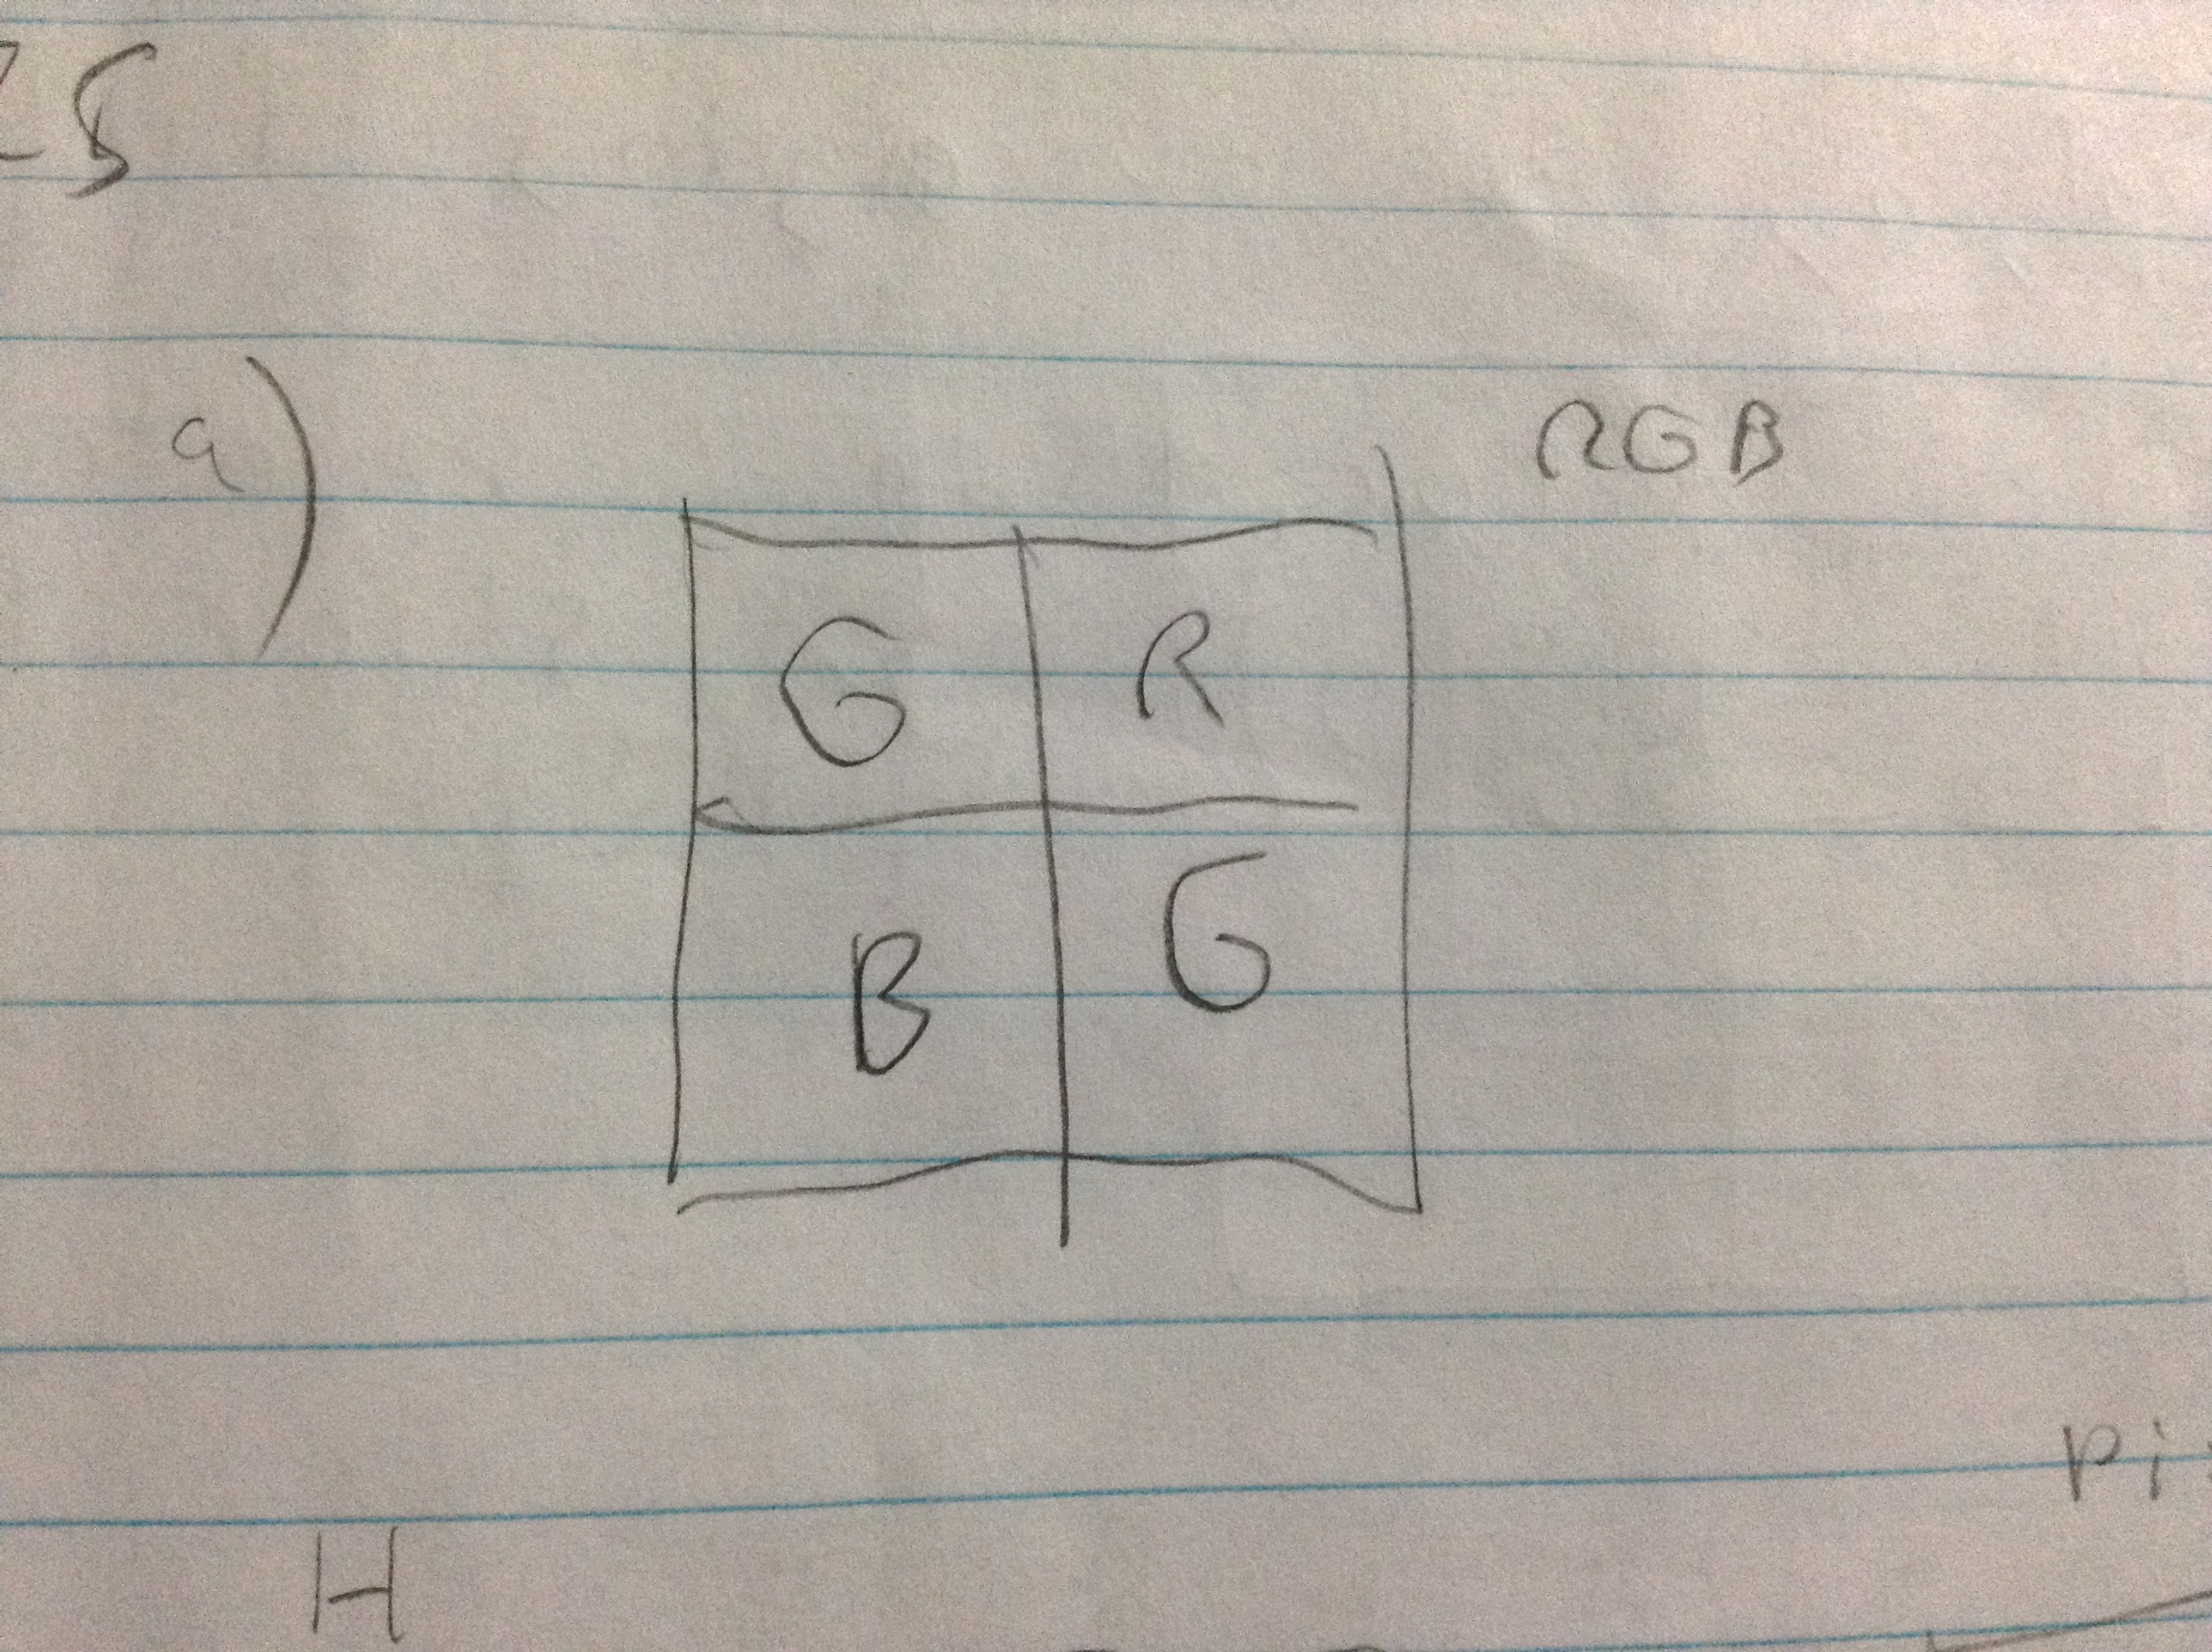
\includegraphics[width=\linewidth]{6.25/fig1.JPG}
		\caption{RGB image}
	\end{figure}
	The colors are said to be fully saturated and to have full intensity.
	Thus the S component of each color is 255, and the I component is .5 or 127.
	\begin{figure}[H]
		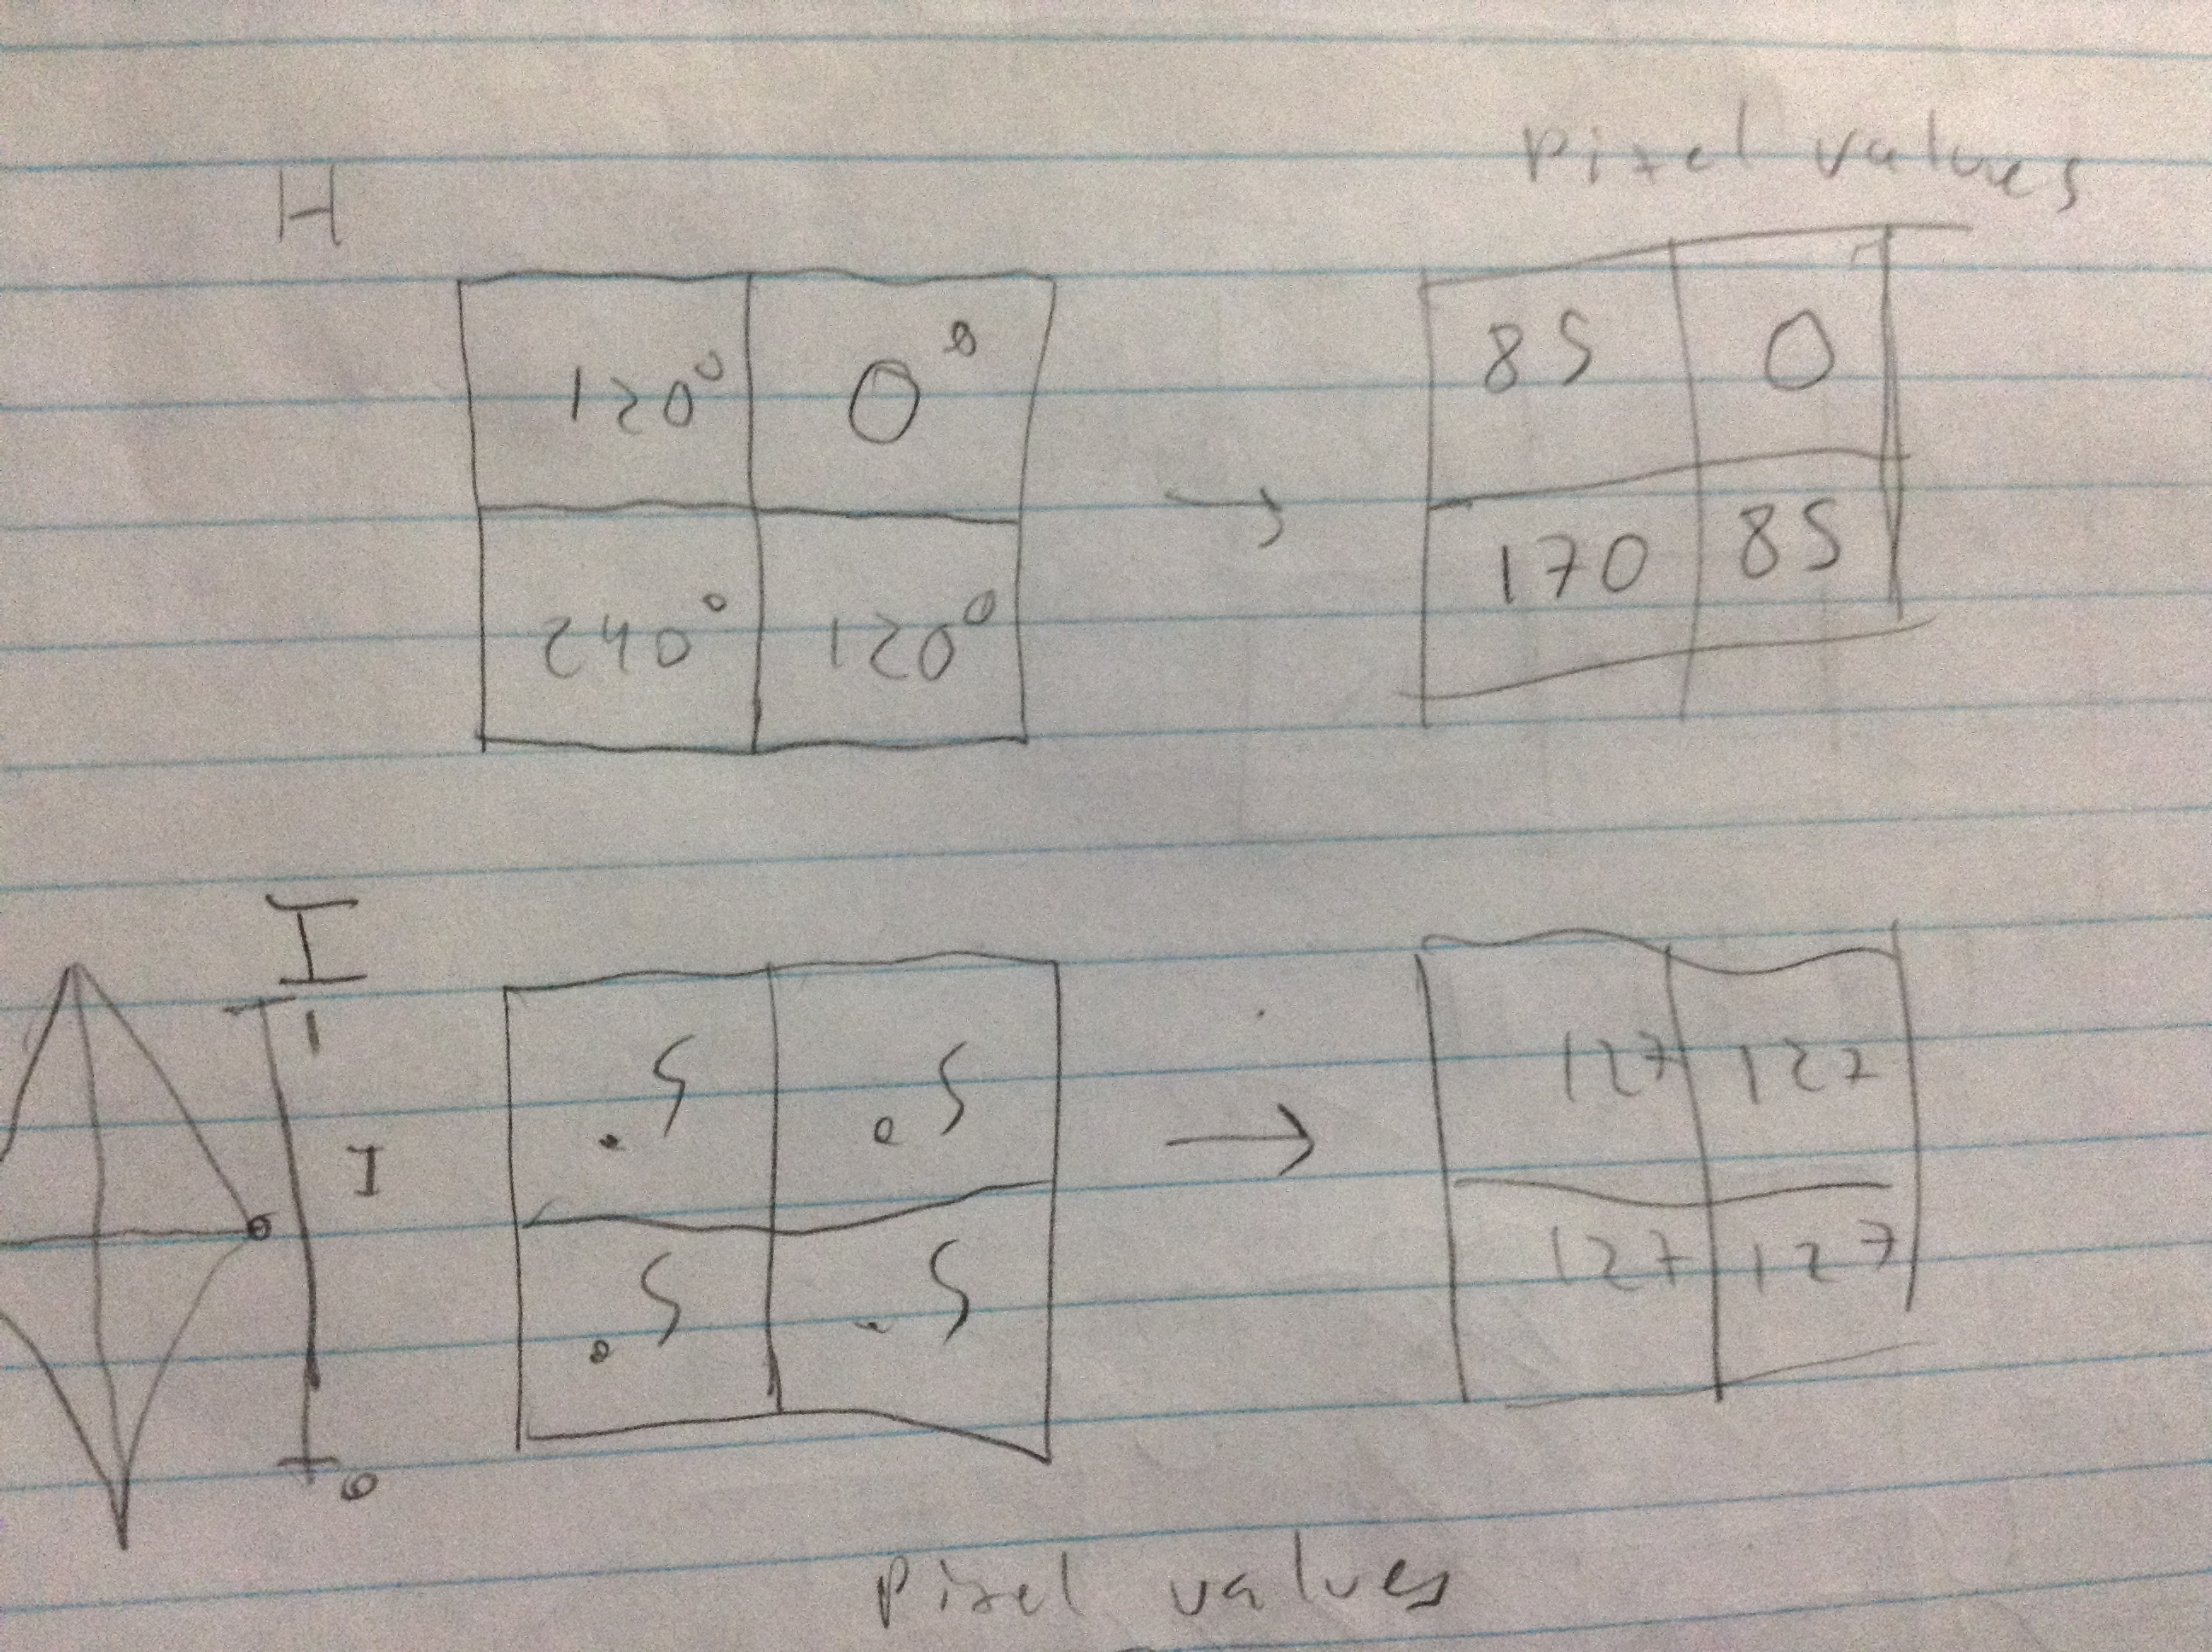
\includegraphics[width=\linewidth]{6.25/fig2.JPG}
		\caption{H and I components}
	\end{figure}
	\begin{figure}[H]
		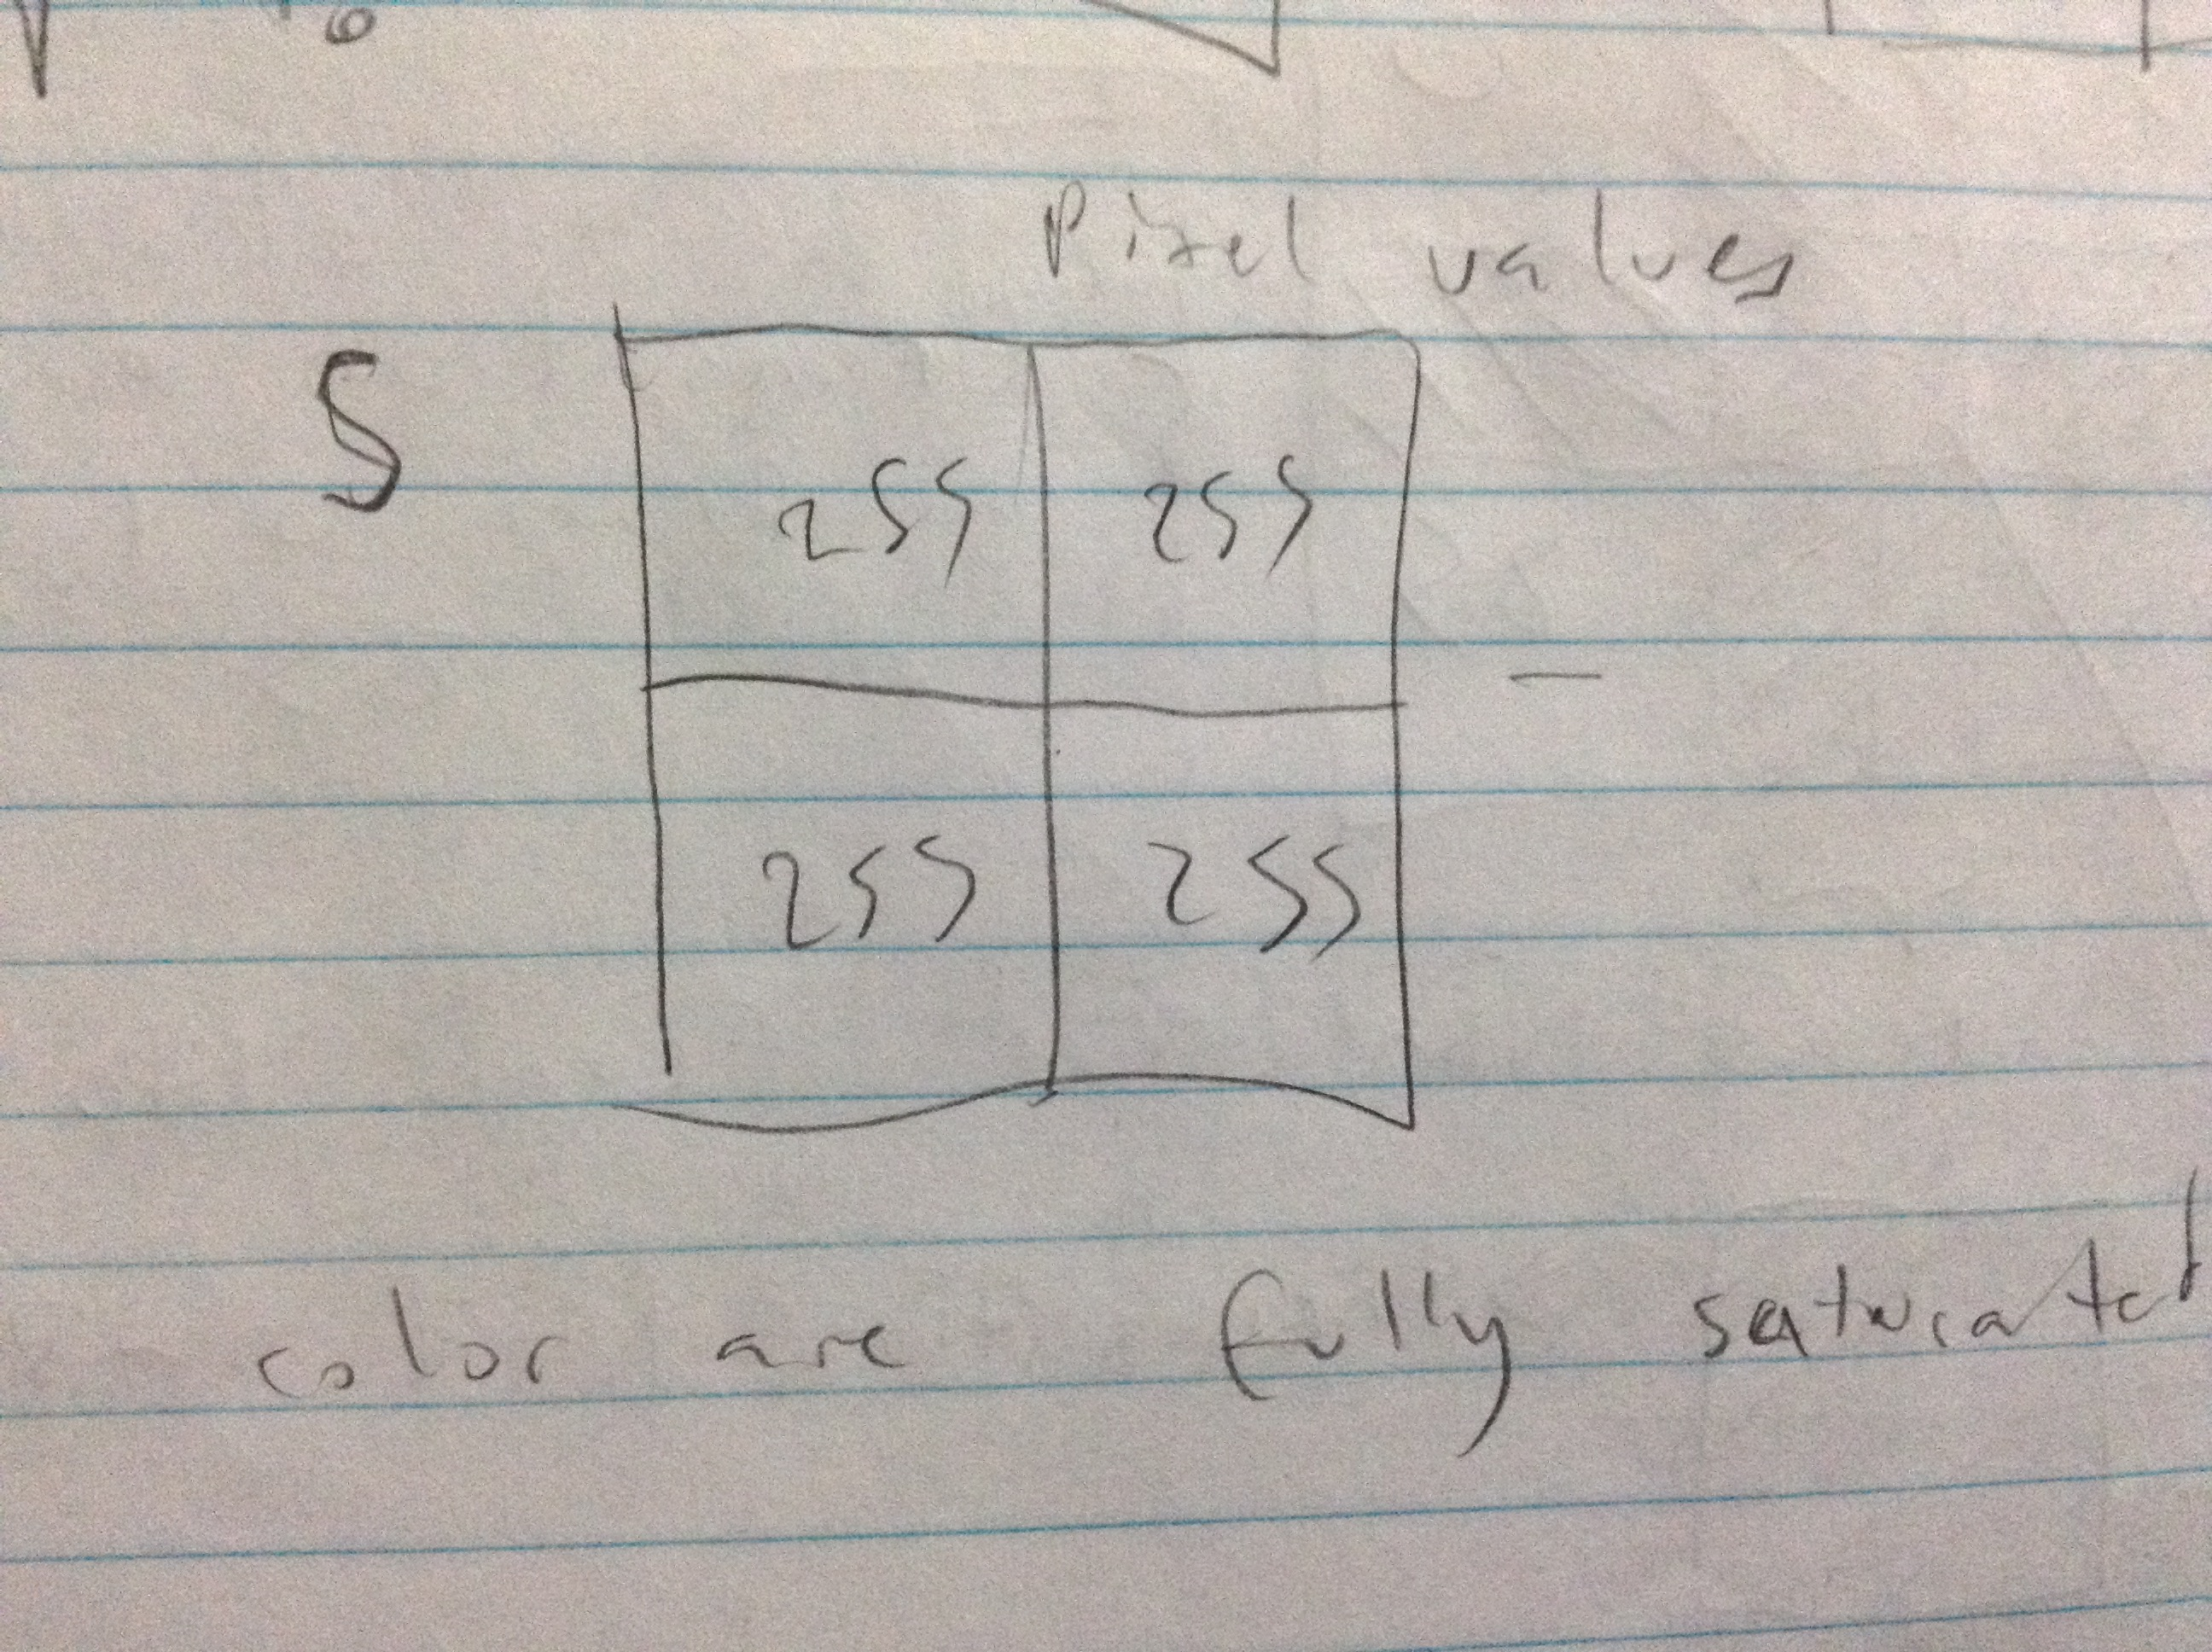
\includegraphics[width=\linewidth]{6.25/fig3.JPG}
		\caption{S component}
	\end{figure}
	
	\subsection{Part b: Describe the appearance of the S component after it is smoothed with an averaging filter}
	The image of the S component remains the same after smoothing, since all of its values are equal.
	\subsection{Part c: Describe the appearance of the H component after it is smoothed with a 250x250 averaging filter}
	\begin{figure}[H]
		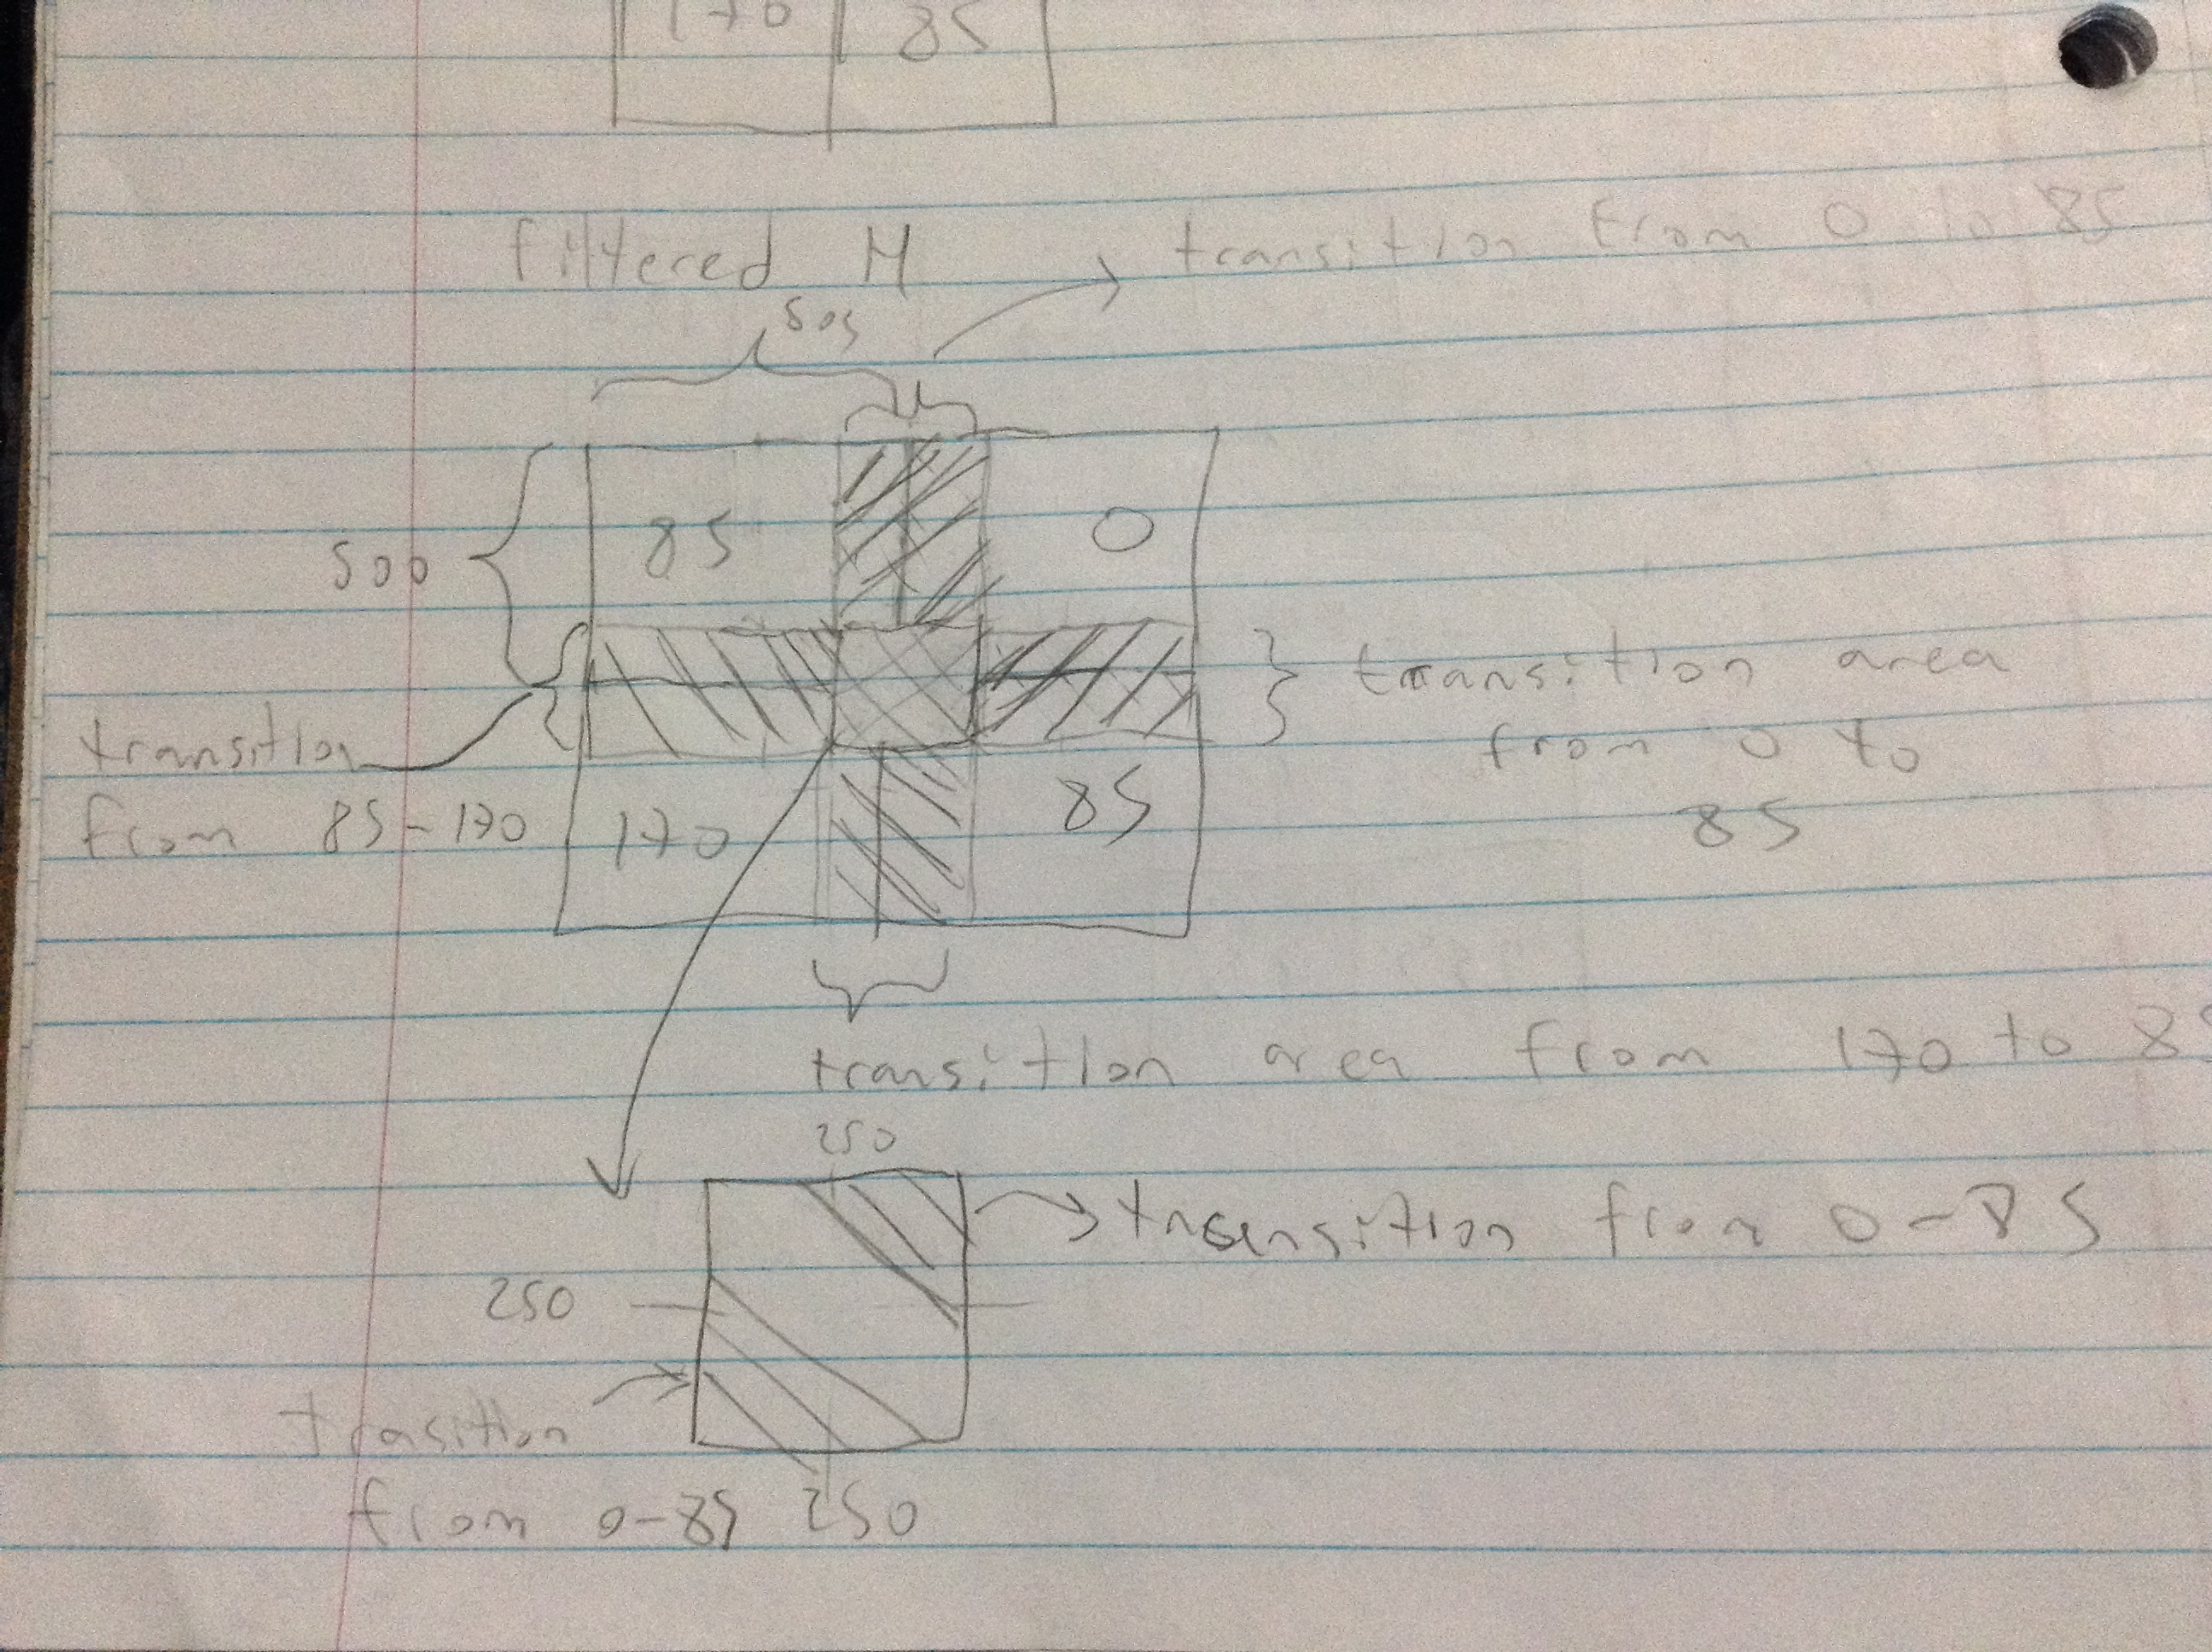
\includegraphics[width=\linewidth]{6.25/fig5.JPG}
		\caption{filtered image}
	\end{figure}
	Filtering produces an image that has transitions where the colors border each other.
	
	\newpage
	\section{Problem 6.25: Sketch the surface}
	\begin{figure}[H]
		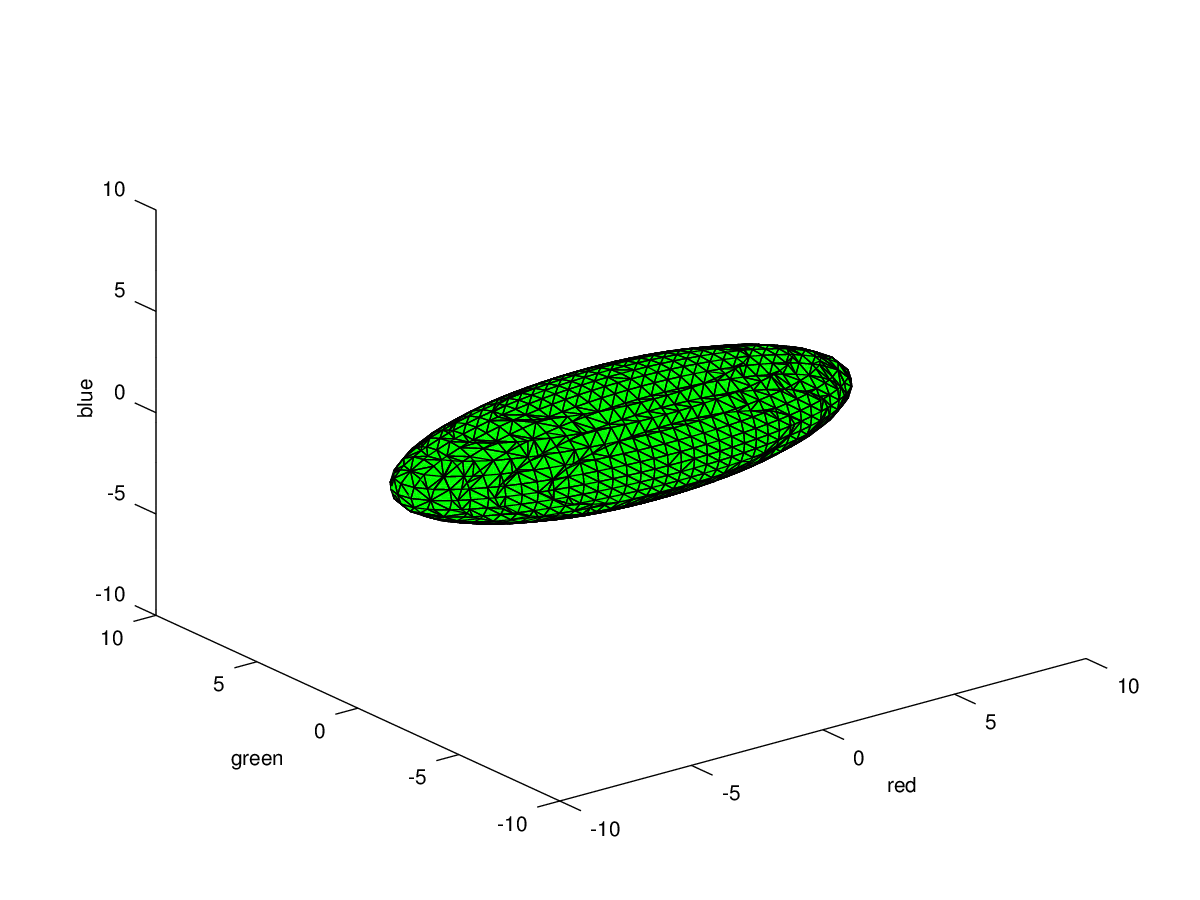
\includegraphics[width=\linewidth]{6.28/part1.png}
		\caption{dilation process}
	\end{figure}
	
	\newpage
	\section{Problem 5}
	\subsection{Part a: Prove the following:}
	\[(A\bullet{B})' = A'\ominus{\hat{B}}\]
	\[(A\oplus{B})' = \{x|(\hat{B})_z\cap{A} \neq{} \emptyset\}'\]
	\[(A\oplus{B})' = \{x|(\hat{B})_z\cap{A} = \emptyset\}\]
	\[A'\ominus{\hat{B}} = \{x|(\hat{B})_z\subseteq{A'}\} \]
	\[A'\ominus{\hat{B}} = \{x|(\hat{B})_z\cap{A} = \emptyset\} \]
	\[(A\bullet{B})' = A'\ominus{\hat{B}}\]
	
	\subsection{Part b: Prove the following:}
	\[(A\bullet{B})' = A'\circ{\hat{B}}\]
	\[(A\bullet{B})' = ((A\oplus{B})\ominus{B})'\]
	\[(A\bullet{B})' = (A\oplus{B})'\oplus{\hat{B}}\]
	\[(A\bullet{B})' = A'\ominus{\hat{B}}\oplus{\hat{B}}\]
	\[(A\bullet{B})' = A'\circ{\hat{B}}\]
	
	\subsection{Part c: Prove the following:}
	\[(A\circ{B})' = A'\bullet{\hat{B}}\]
	\[(A\circ{B})' = ((A\ominus{B})\oplus{B})'\]
	\[(A\circ{B})' = (A\ominus{B})'\ominus{\hat{B}}\]
	\[(A\circ{B})' = A'\oplus{\hat{B}}\ominus{\hat{B}}\]
	\[(A\circ{B})' = A'\bullet{\hat{B}}\]
	
	\newpage
	\section{Problem 6}
	\subsection{Part a: Dilate the image by hand}
	\begin{figure}[H]
		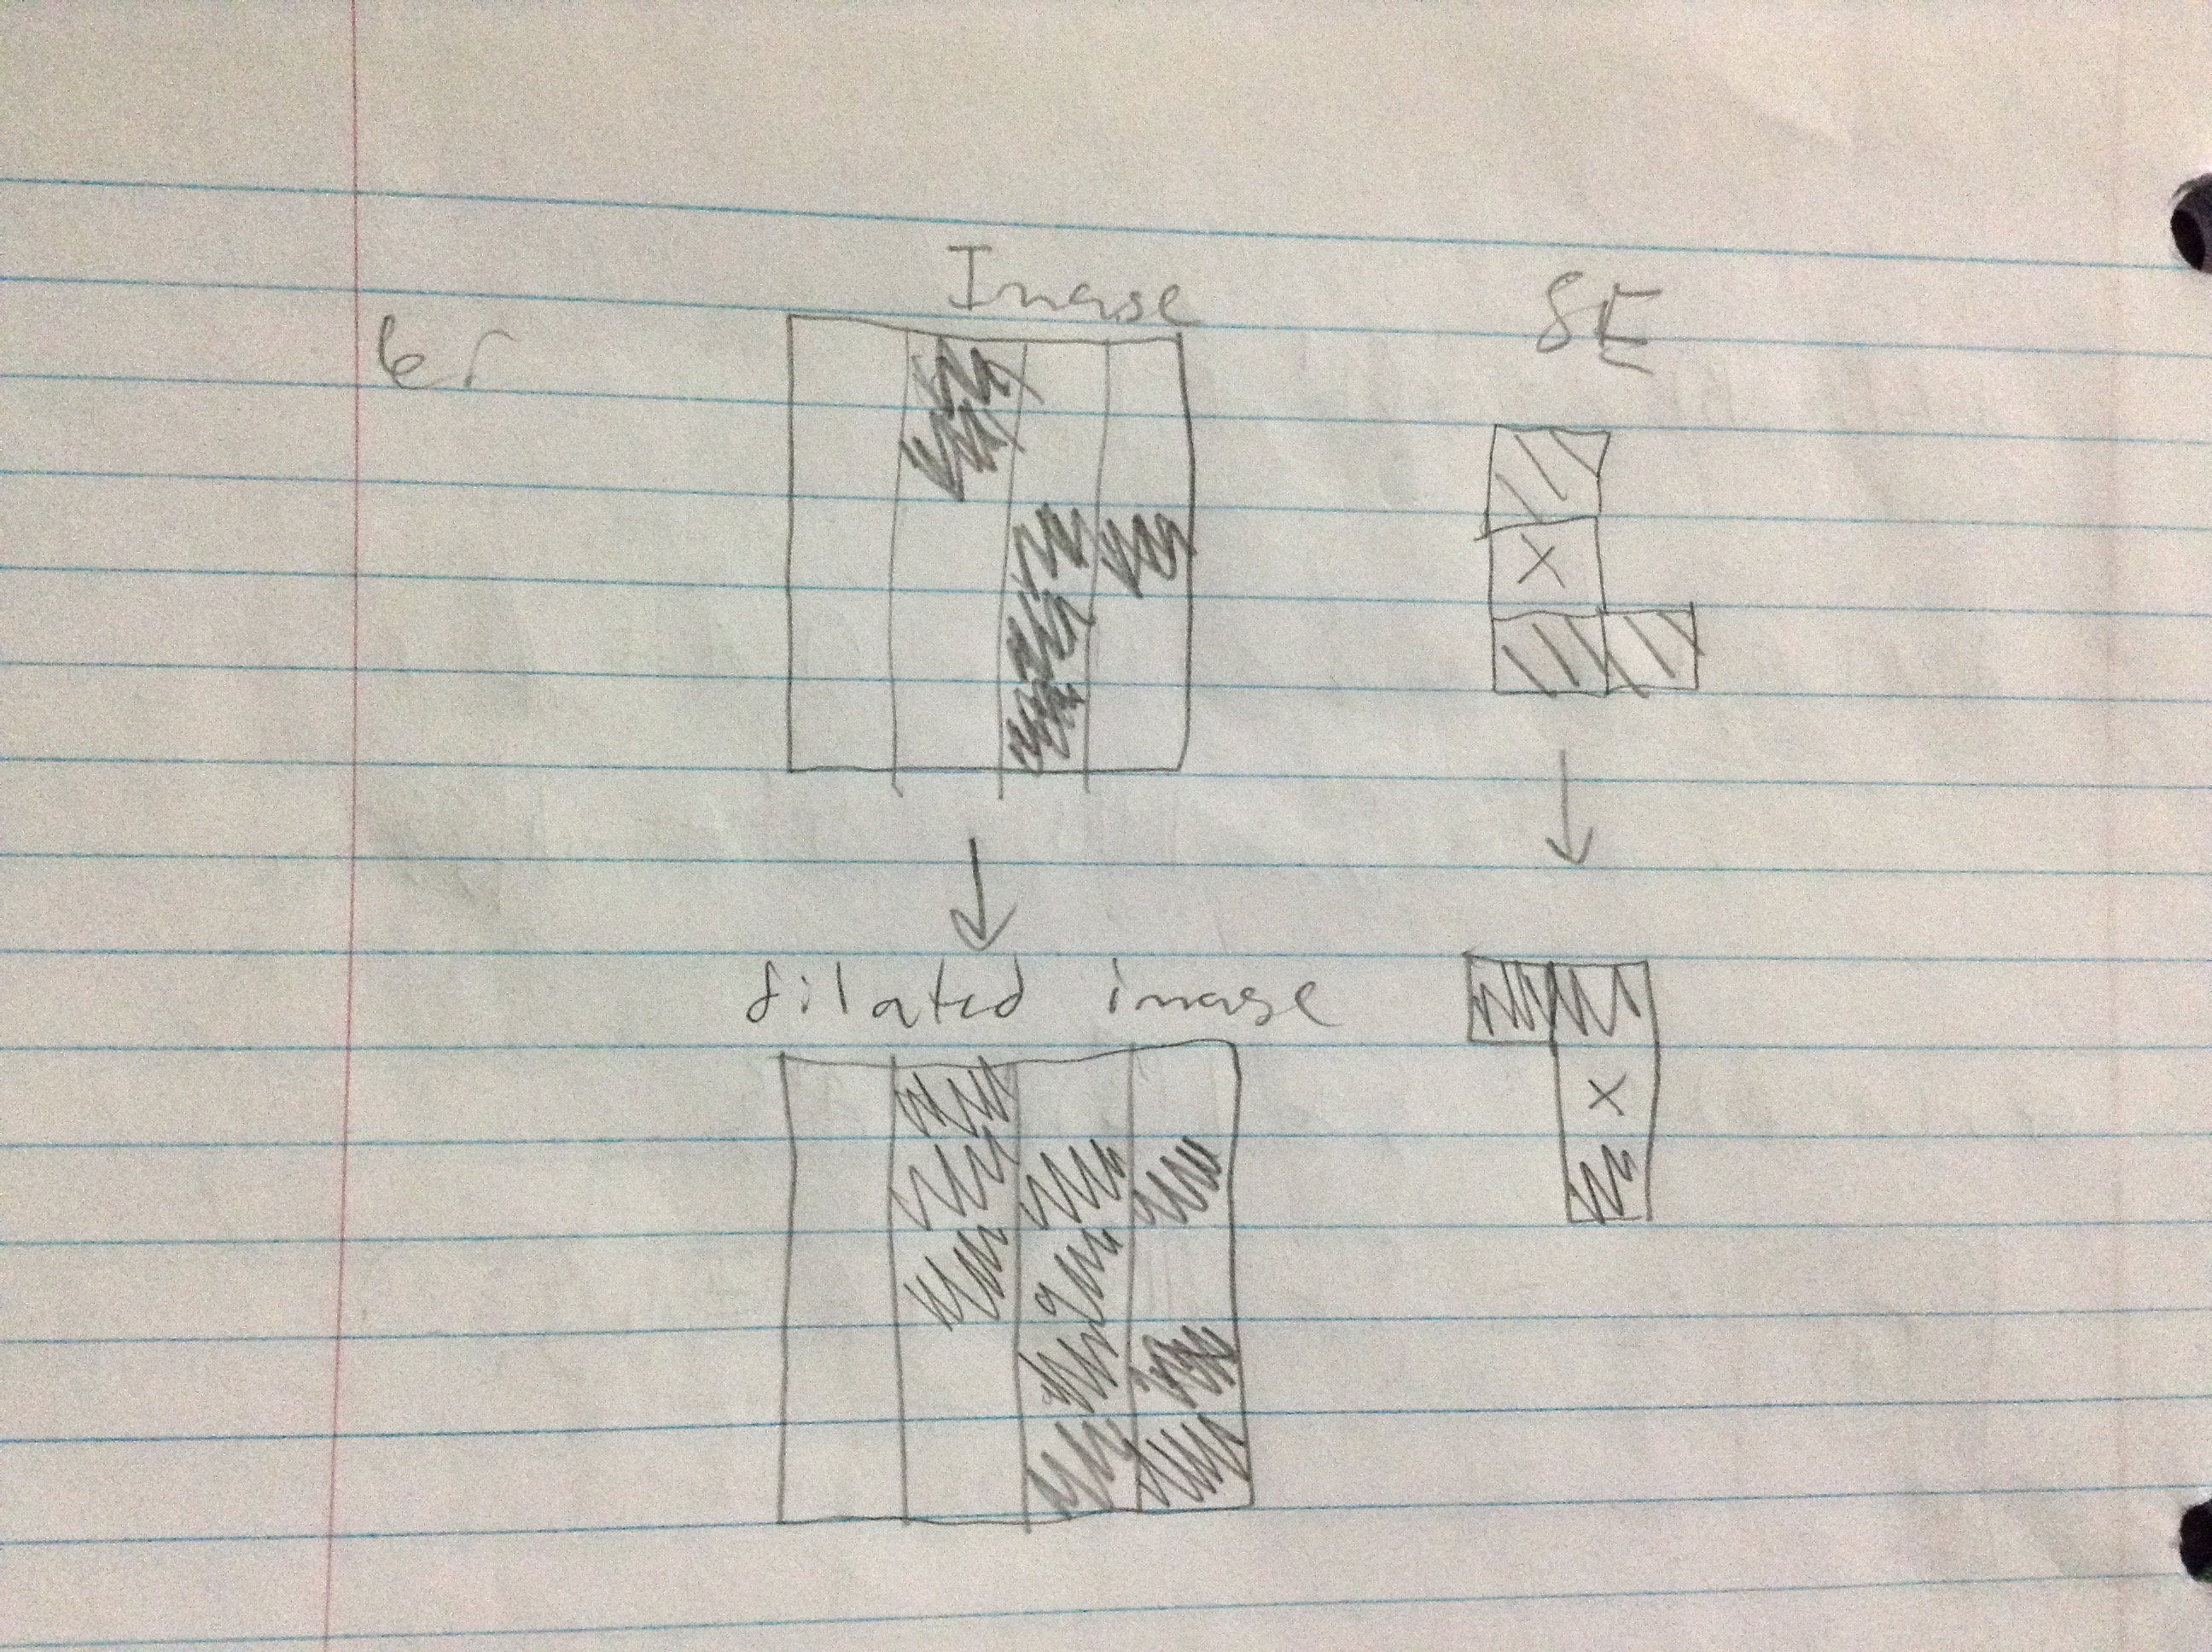
\includegraphics[width=\linewidth]{Q6/fig1.JPG}
		\caption{dilation process}
	\end{figure}
	In the drawn image black represents items in the set. While in the matlab images white represents items in the set.
	\subsection{Part b: Dilate the image using Matlab}
	\begin{figure}[H]
		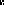
\includegraphics[width=\linewidth]{Q6/original.png}
		\caption{original image}
	\end{figure}
	\begin{figure}[H]
		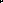
\includegraphics[width=\linewidth]{Q6/SE.png}
		\caption{structural element}
	\end{figure}
	\begin{figure}[H]
		
\includegraphics[width=\linewidth]{Q6/dilated.png}
		\caption{dilated image}
	\end{figure}
	
	\newpage
	\section{Problem 2.23}
	\subsection{Sketch the set given by the expression}
	\begin{figure}[H]
		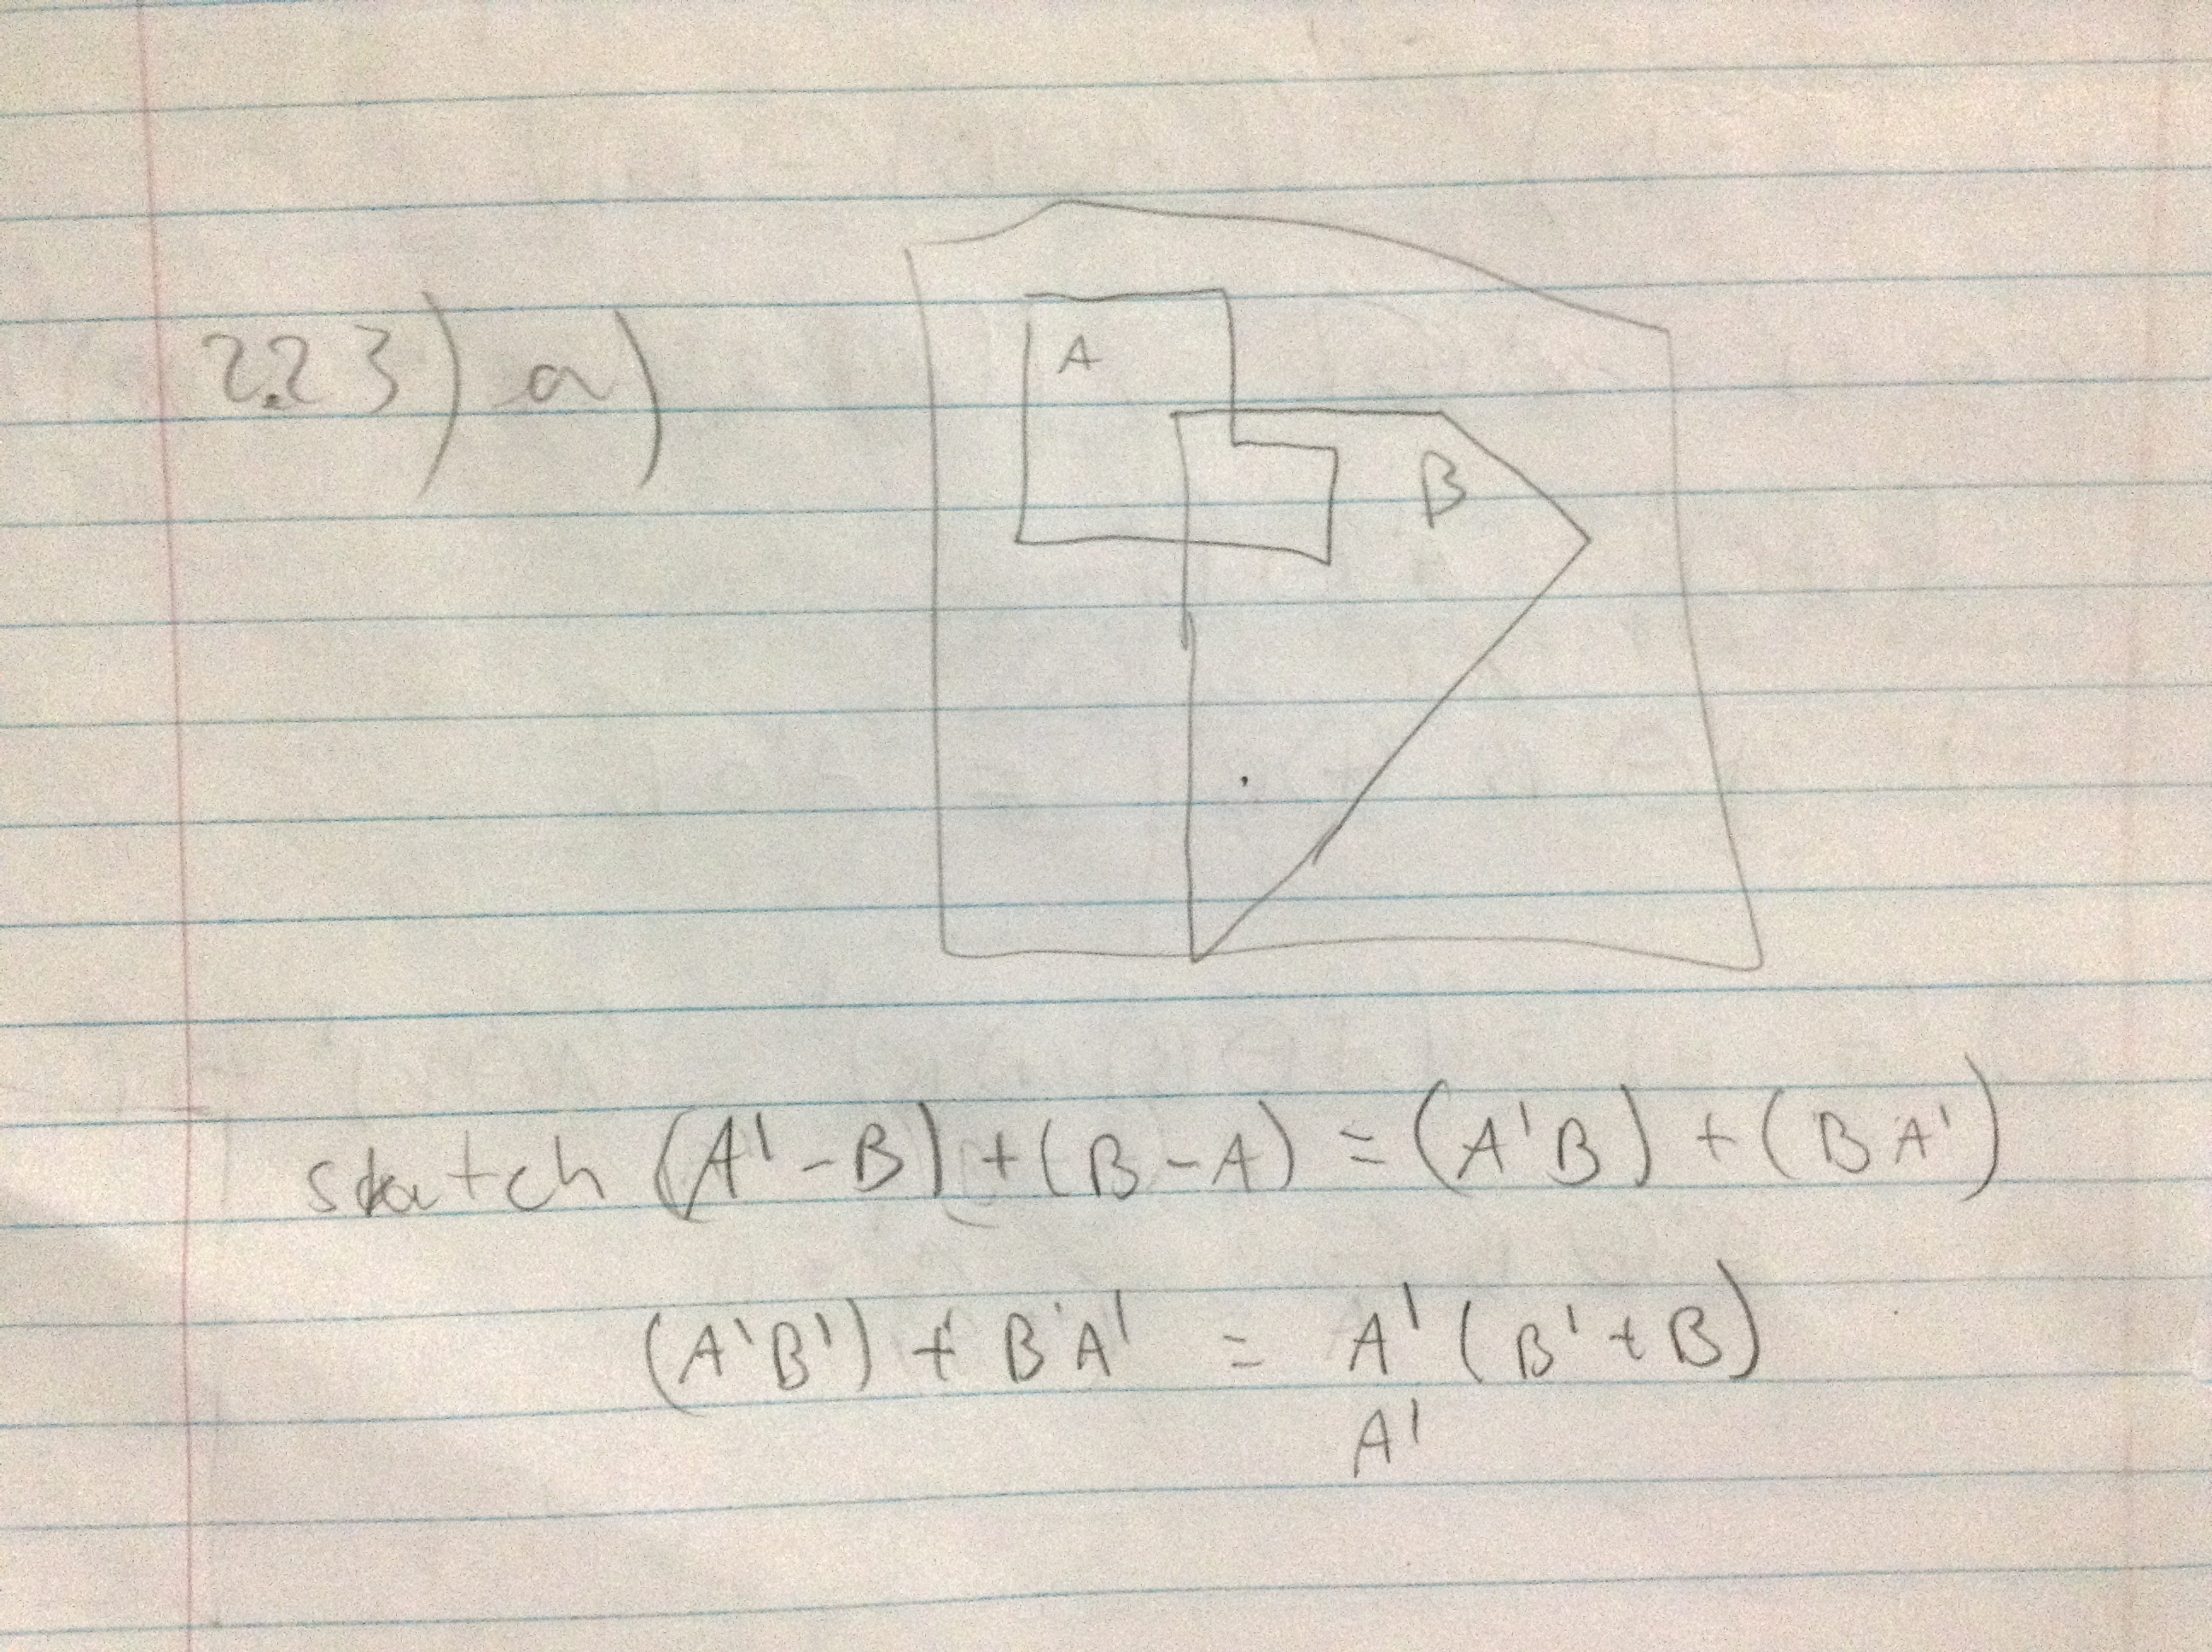
\includegraphics[width=\linewidth]{2.23/fig1.JPG}
		\caption{set a and b}
	\end{figure}
	\begin{figure}[H]
		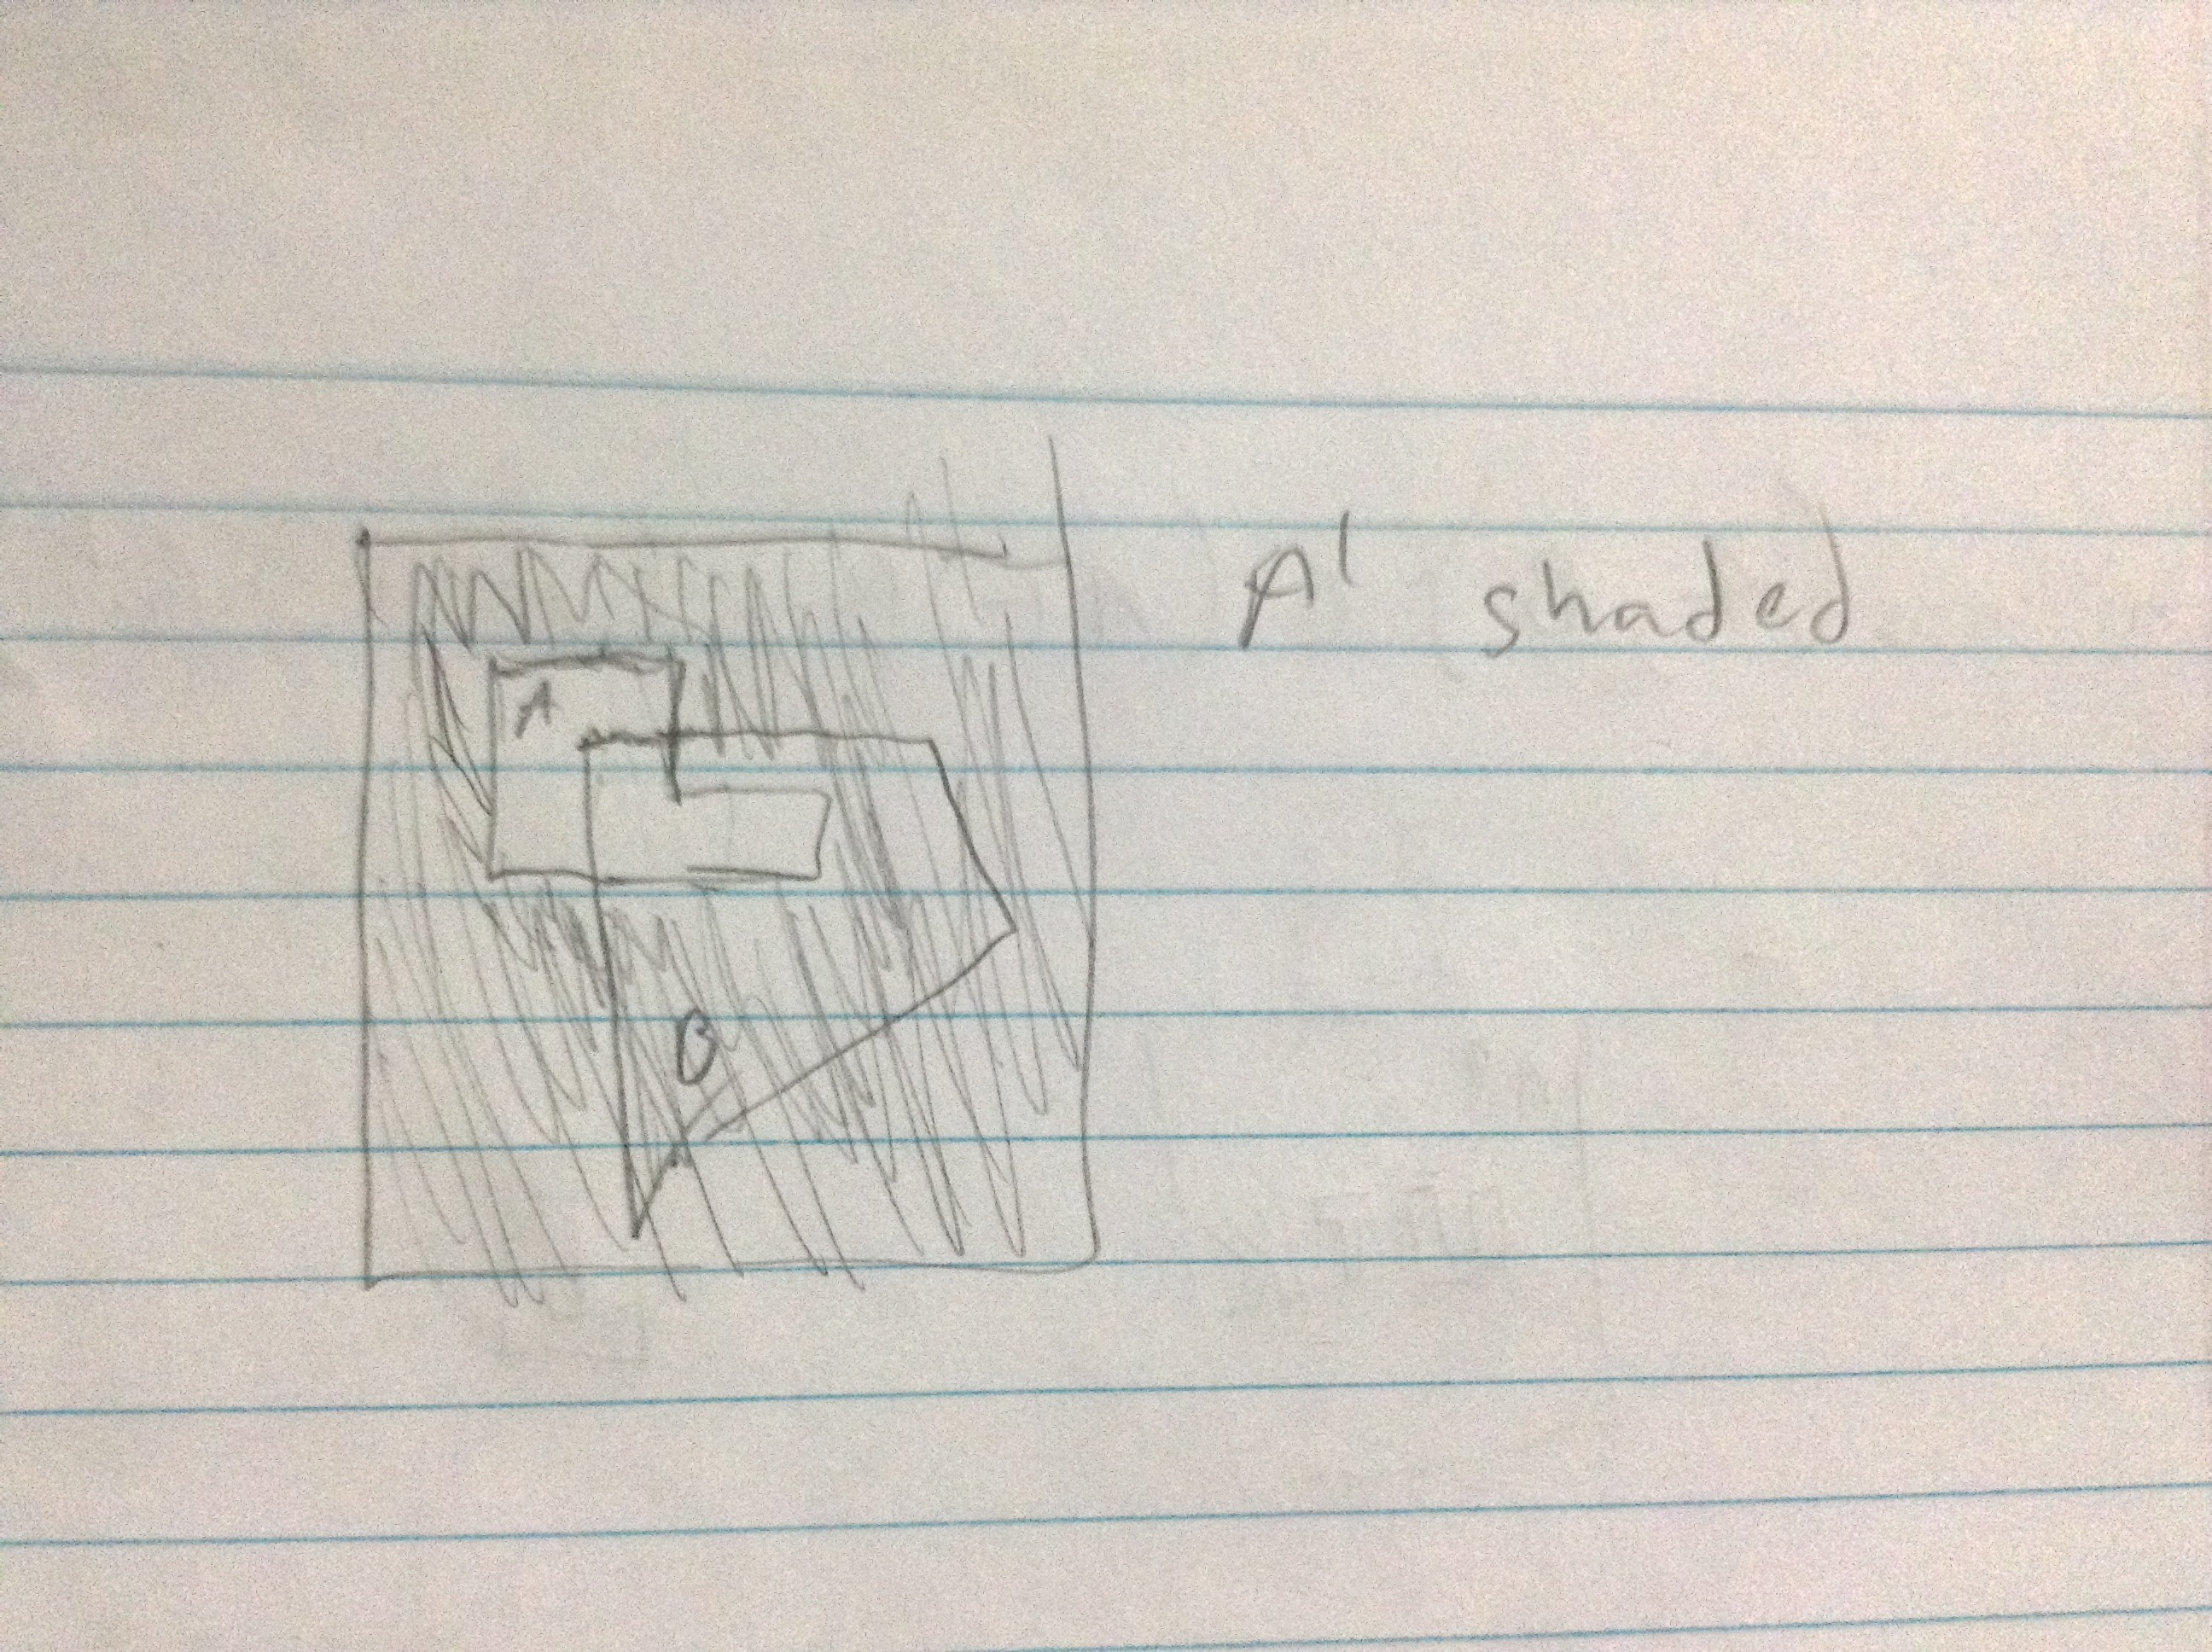
\includegraphics[width=\linewidth]{2.23/fig2.JPG}
		\caption{sketch of expression}
	\end{figure}
	\subsection{Give expressions for the shaded regions}
	\begin{figure}[H]
		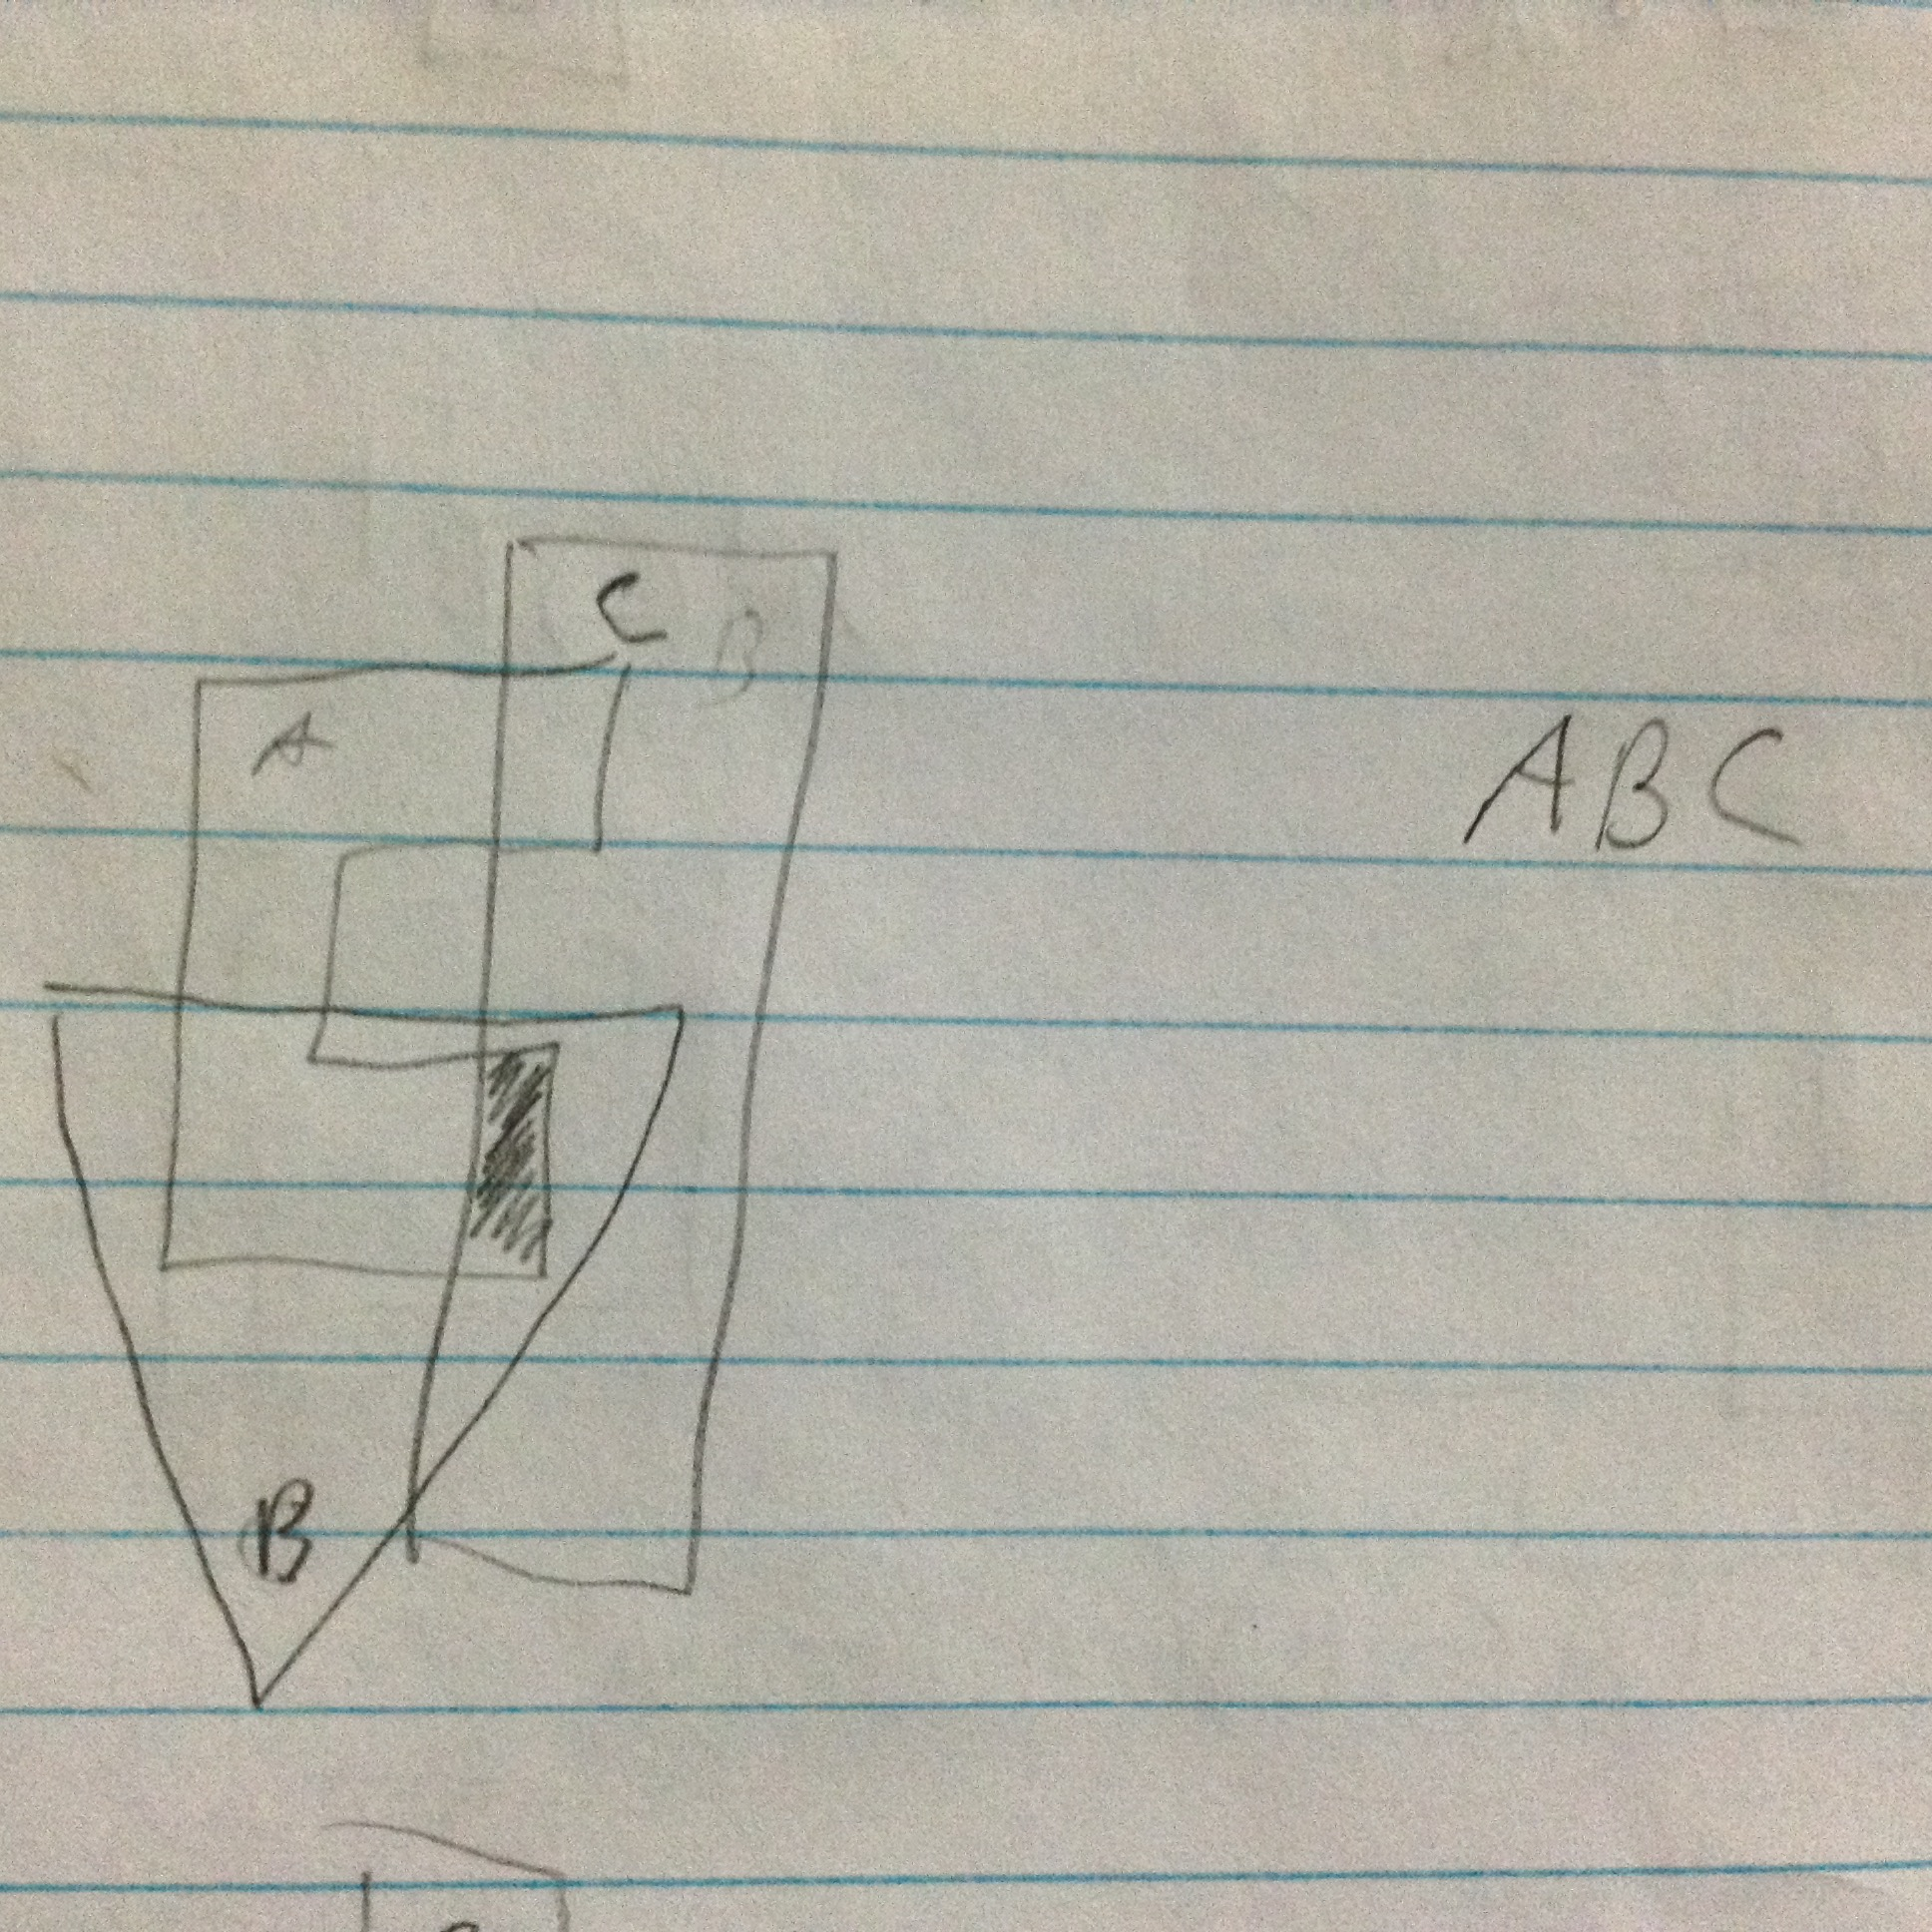
\includegraphics[width=\linewidth]{2.23/fig3.JPG}
		\caption{shaded region of a, b, and c}
	\end{figure}
	\begin{figure}[H]
		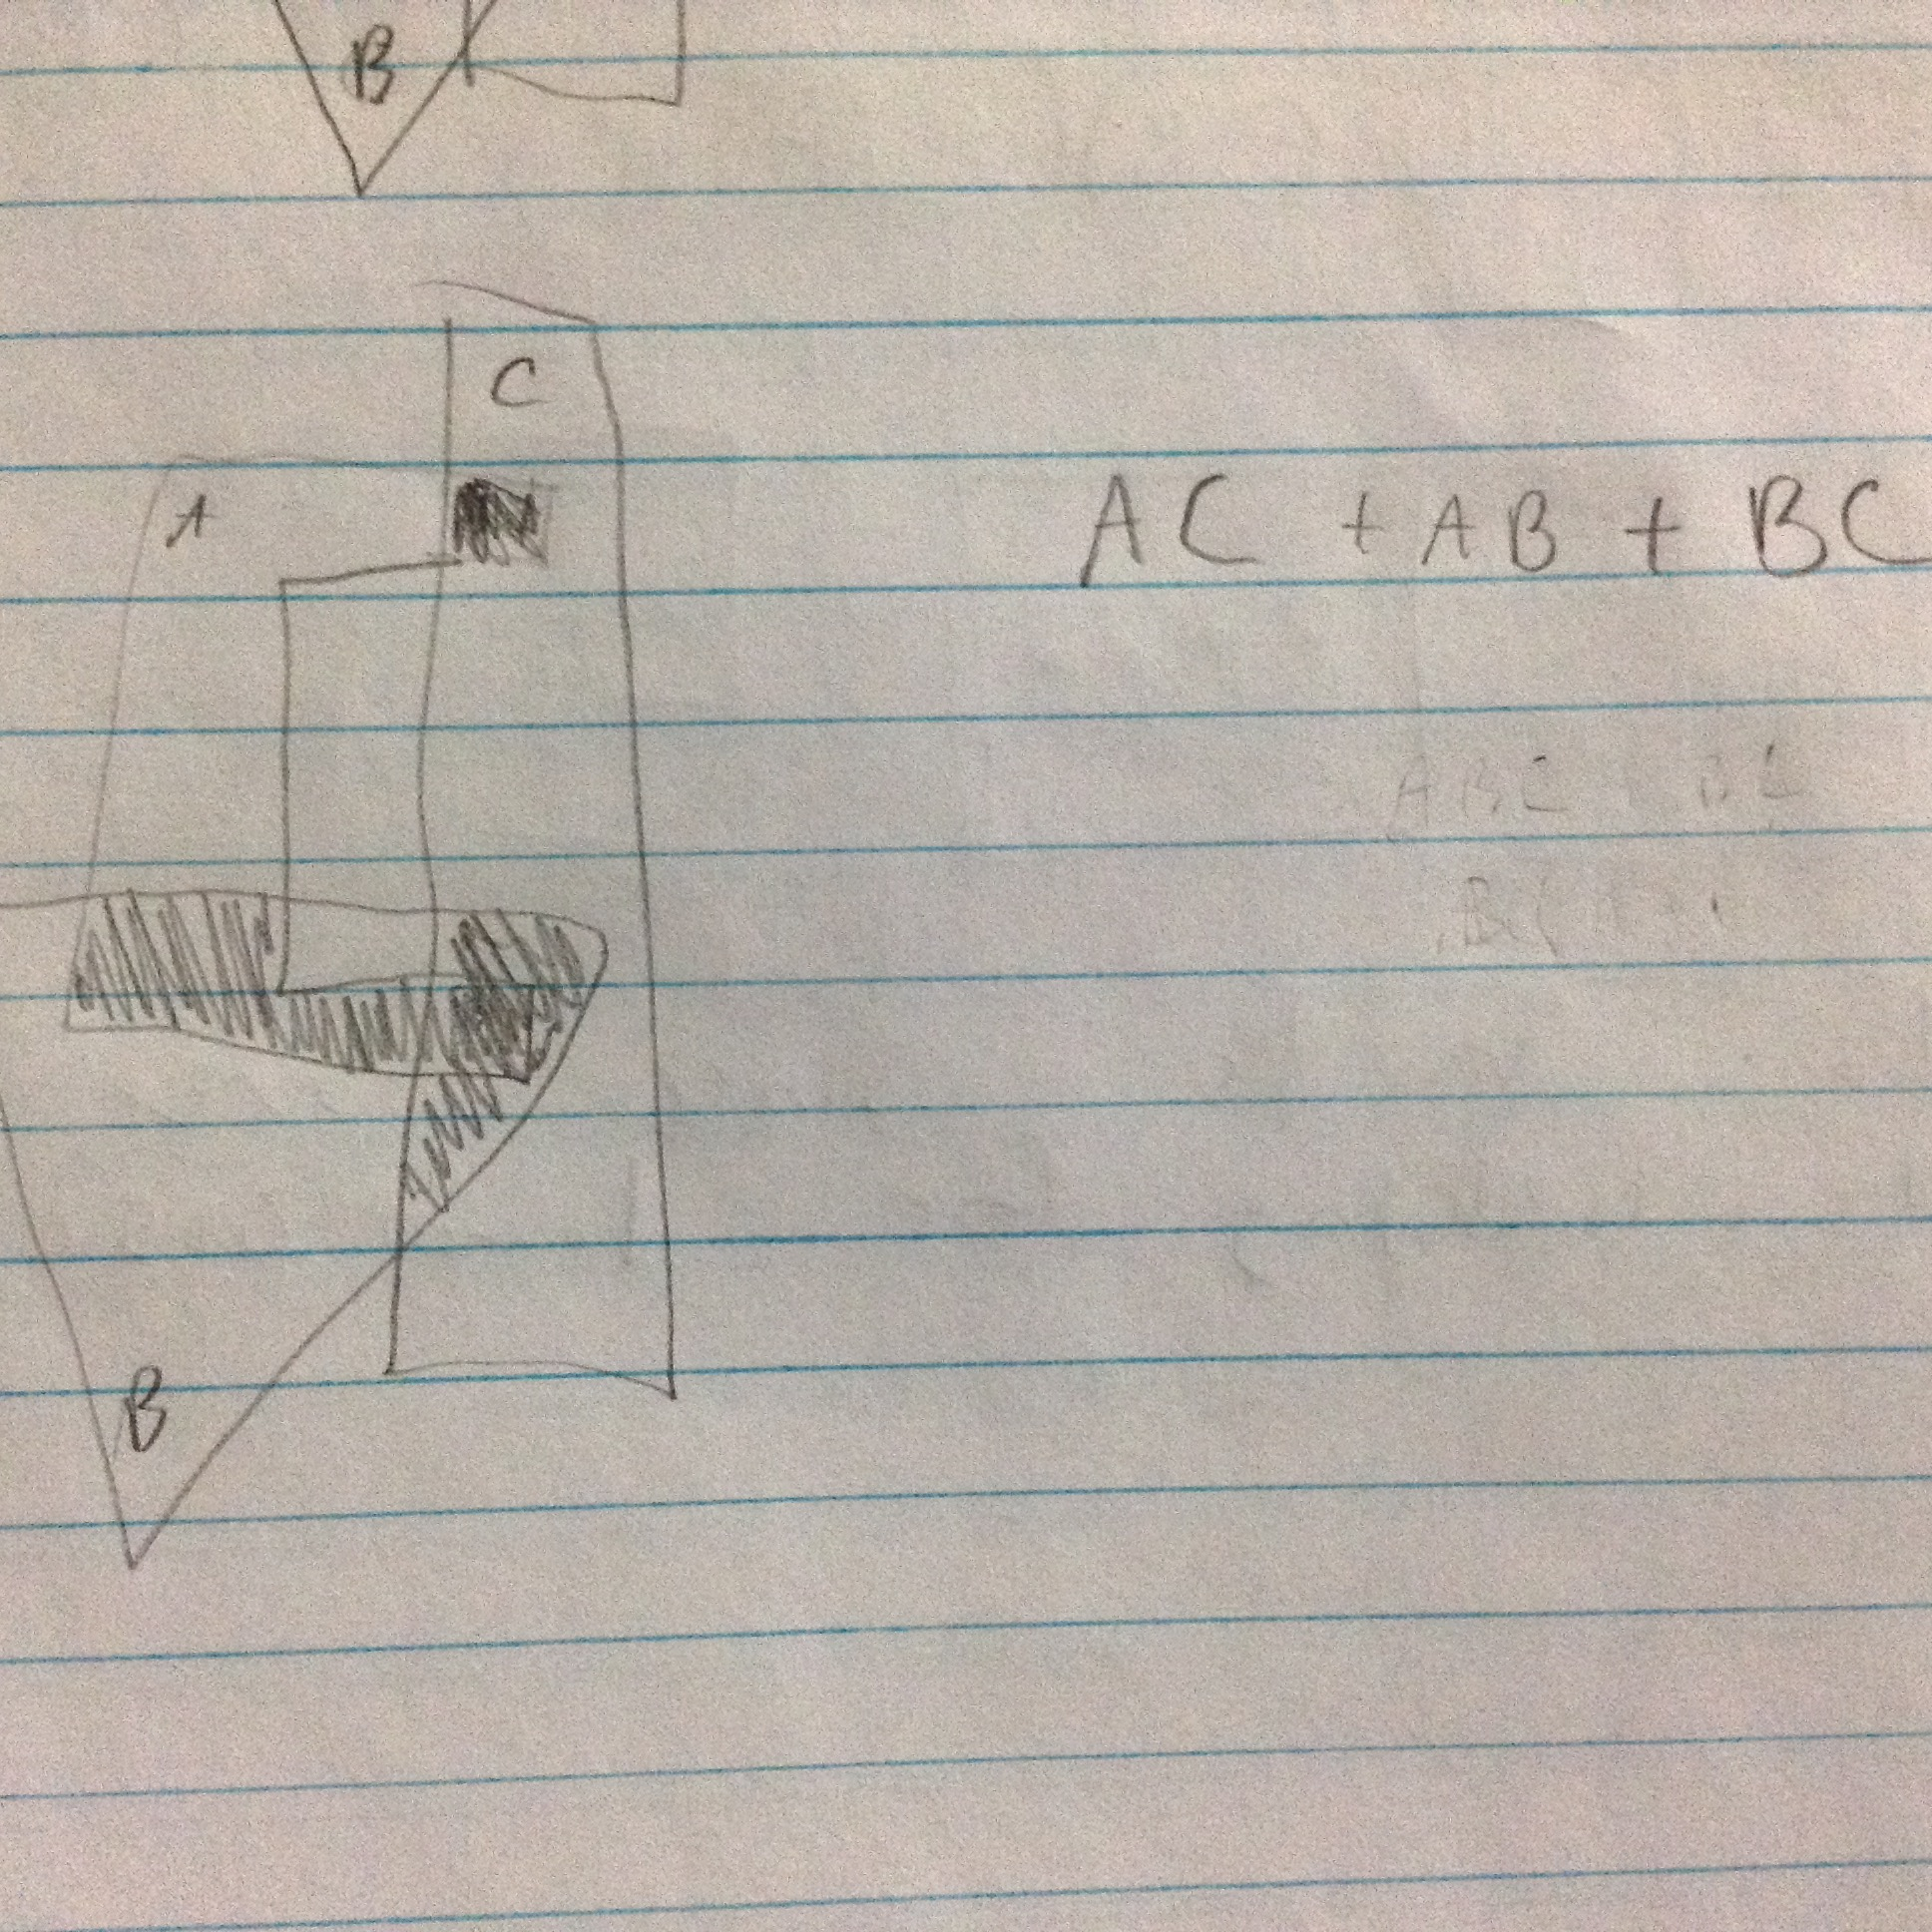
\includegraphics[width=\linewidth]{2.23/fig4.JPG}
		\caption{shaded region of a, b, and c}
	\end{figure}
	\begin{figure}[H]
		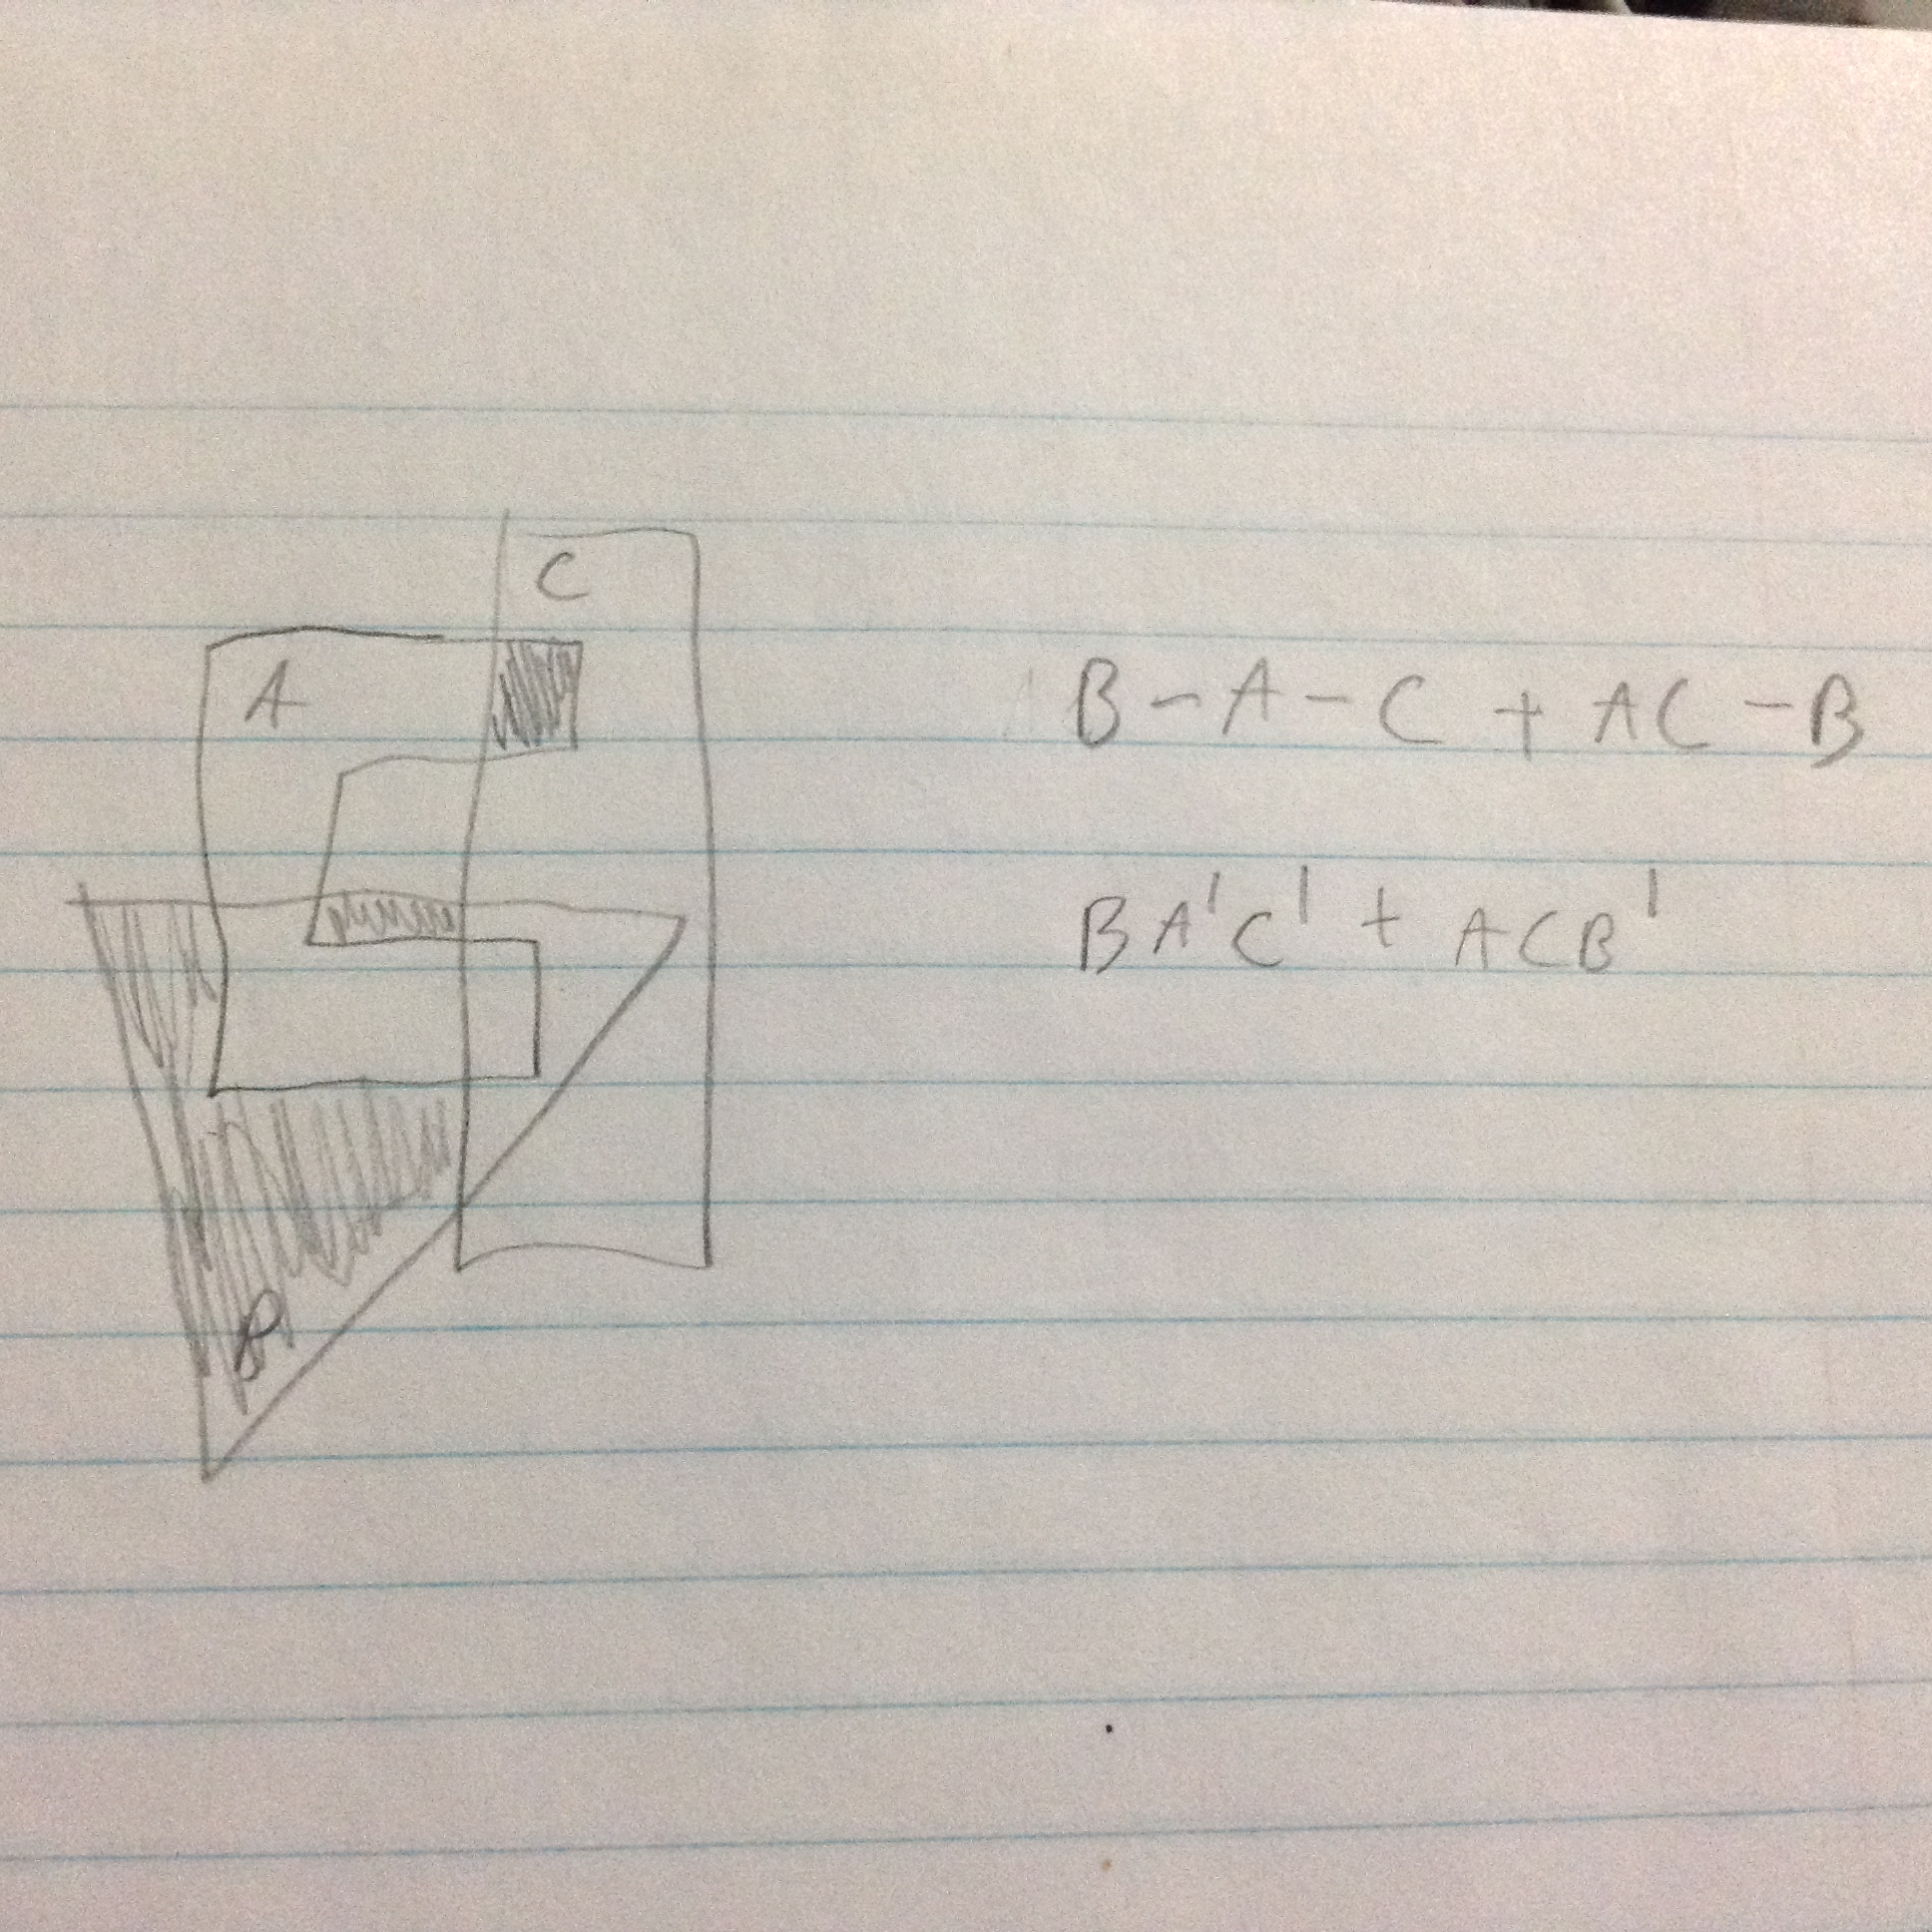
\includegraphics[width=\linewidth]{2.23/fig5.JPG}
		\caption{shaded region of a, b, and c}
	\end{figure}
	
	\newpage
	\section{Problem 9.5: Give structuring element and operation needed to produce the second image from the first}
	\subsection{Part a}
	\begin{figure}[H]
		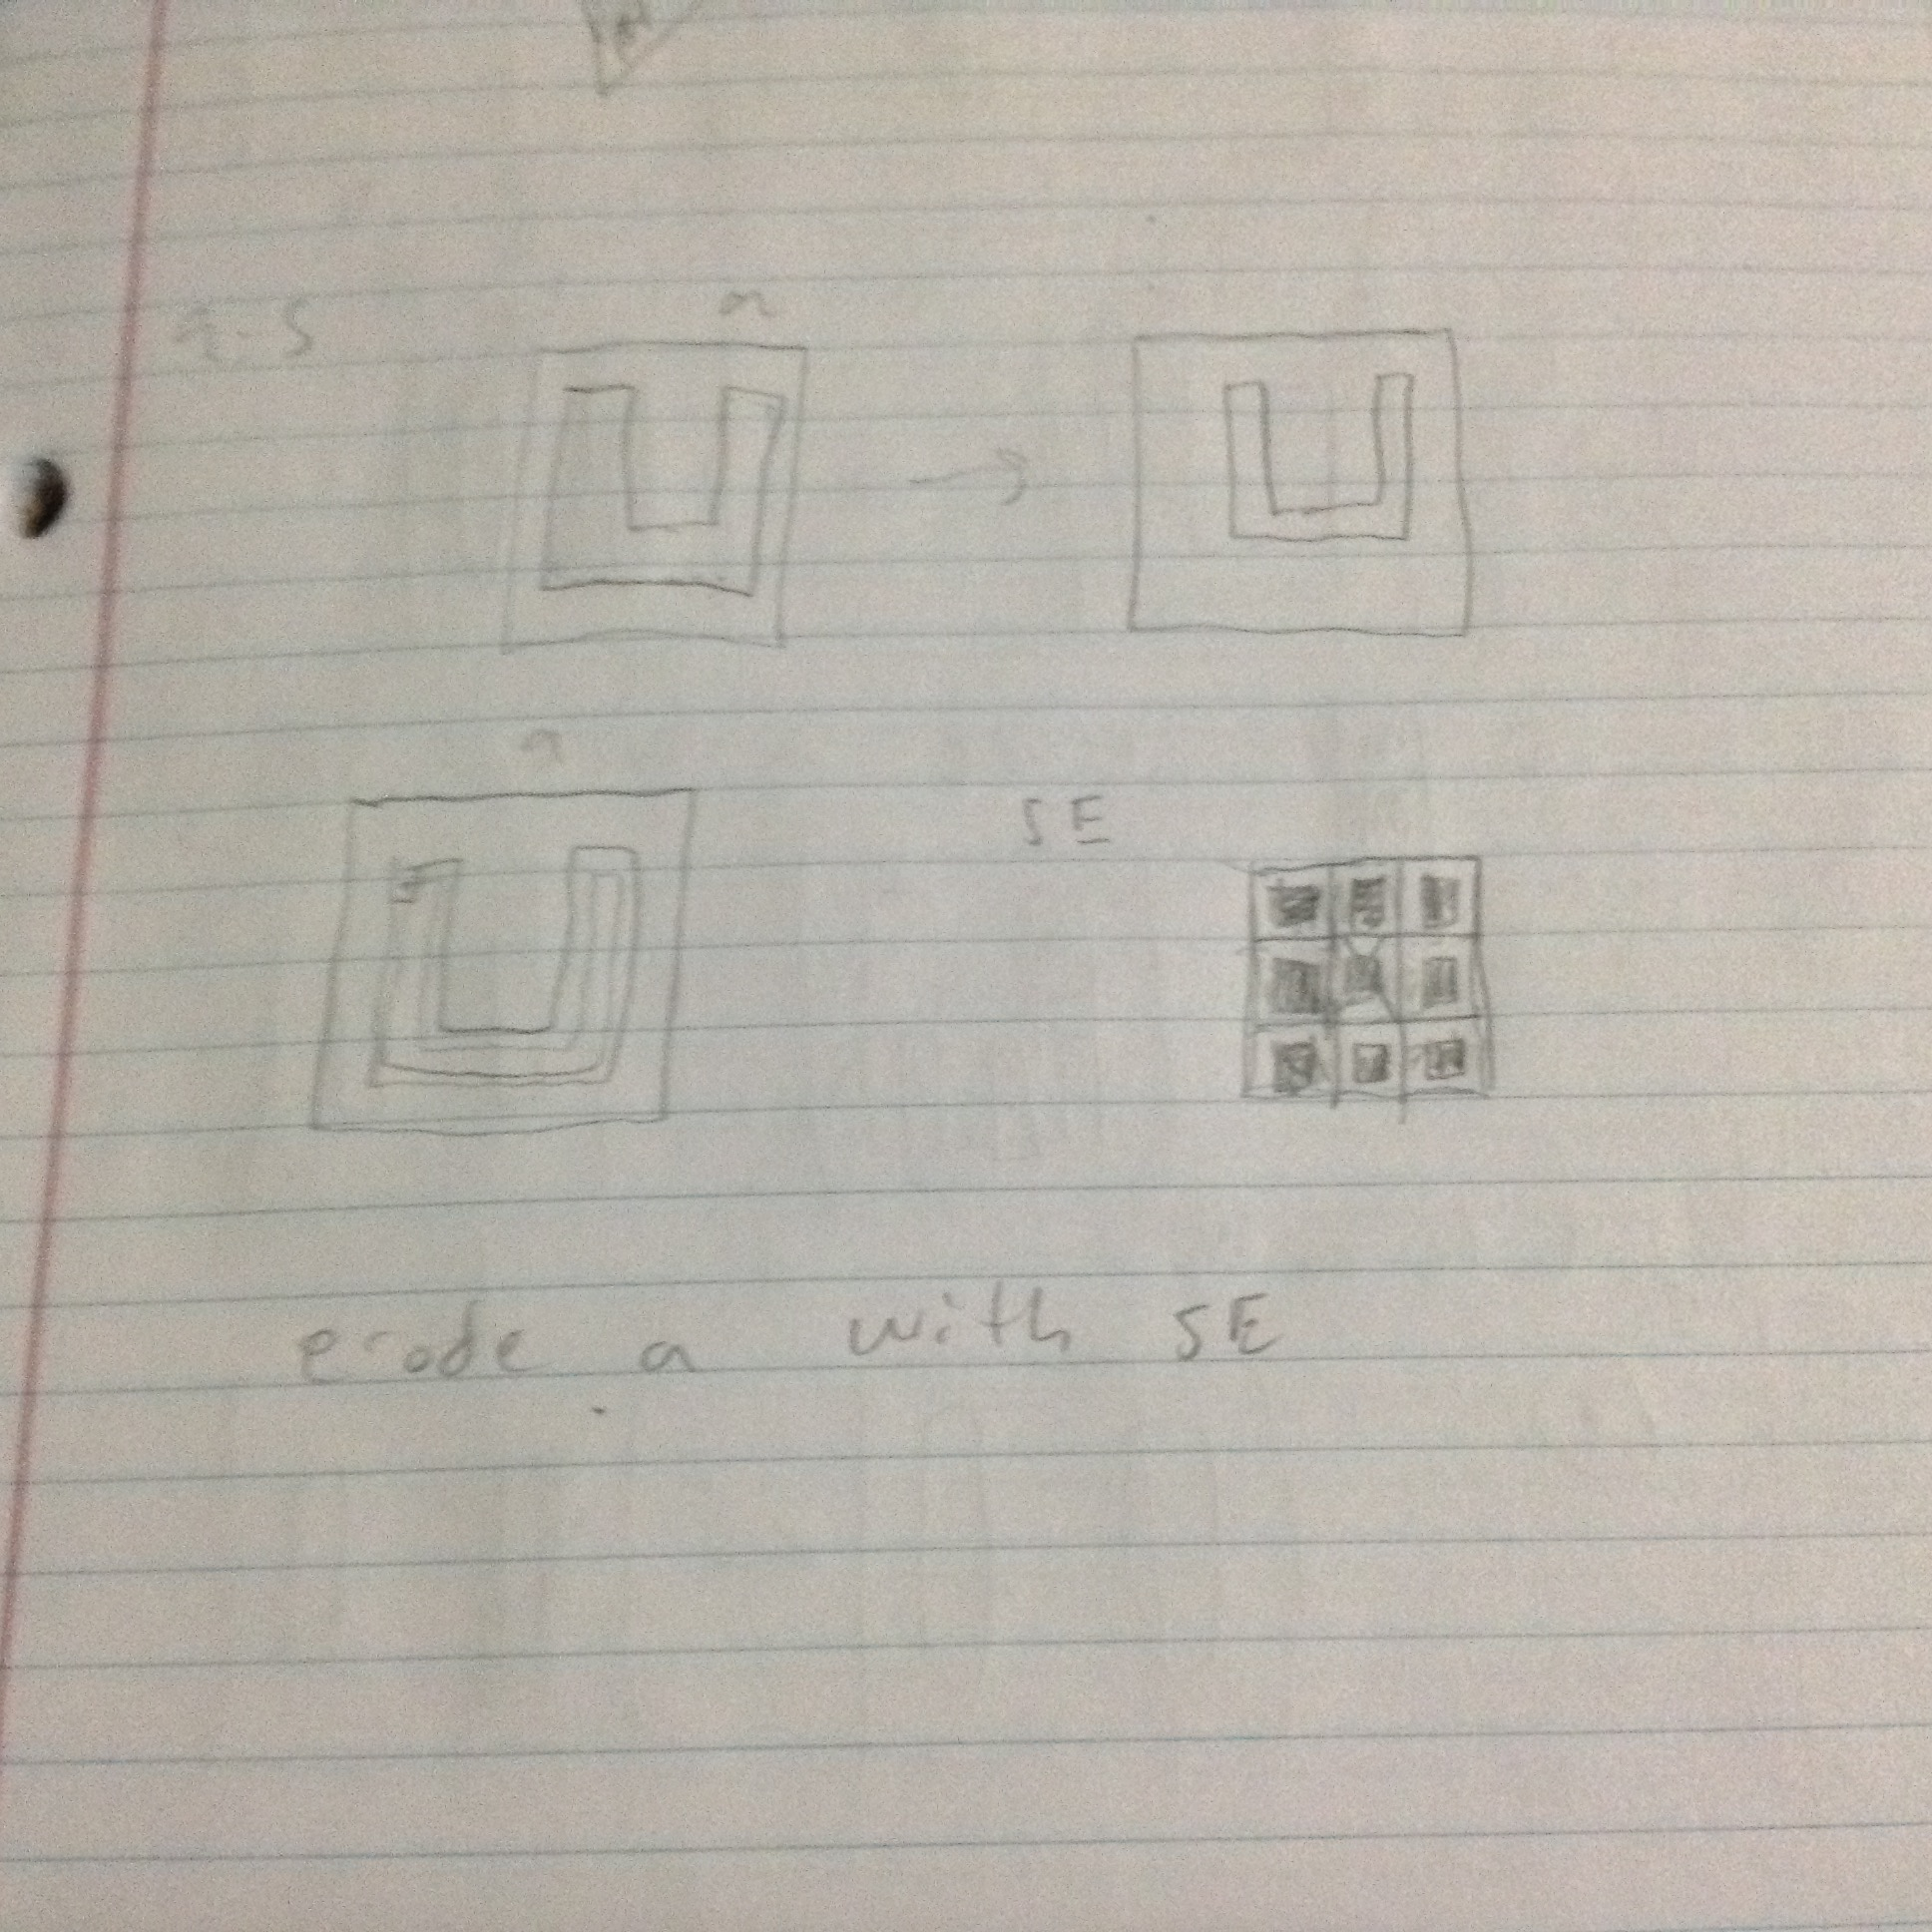
\includegraphics[width=\linewidth]{9.5/fig1.JPG}
	\end{figure}
	\subsection{Part b}
	\begin{figure}[H]
		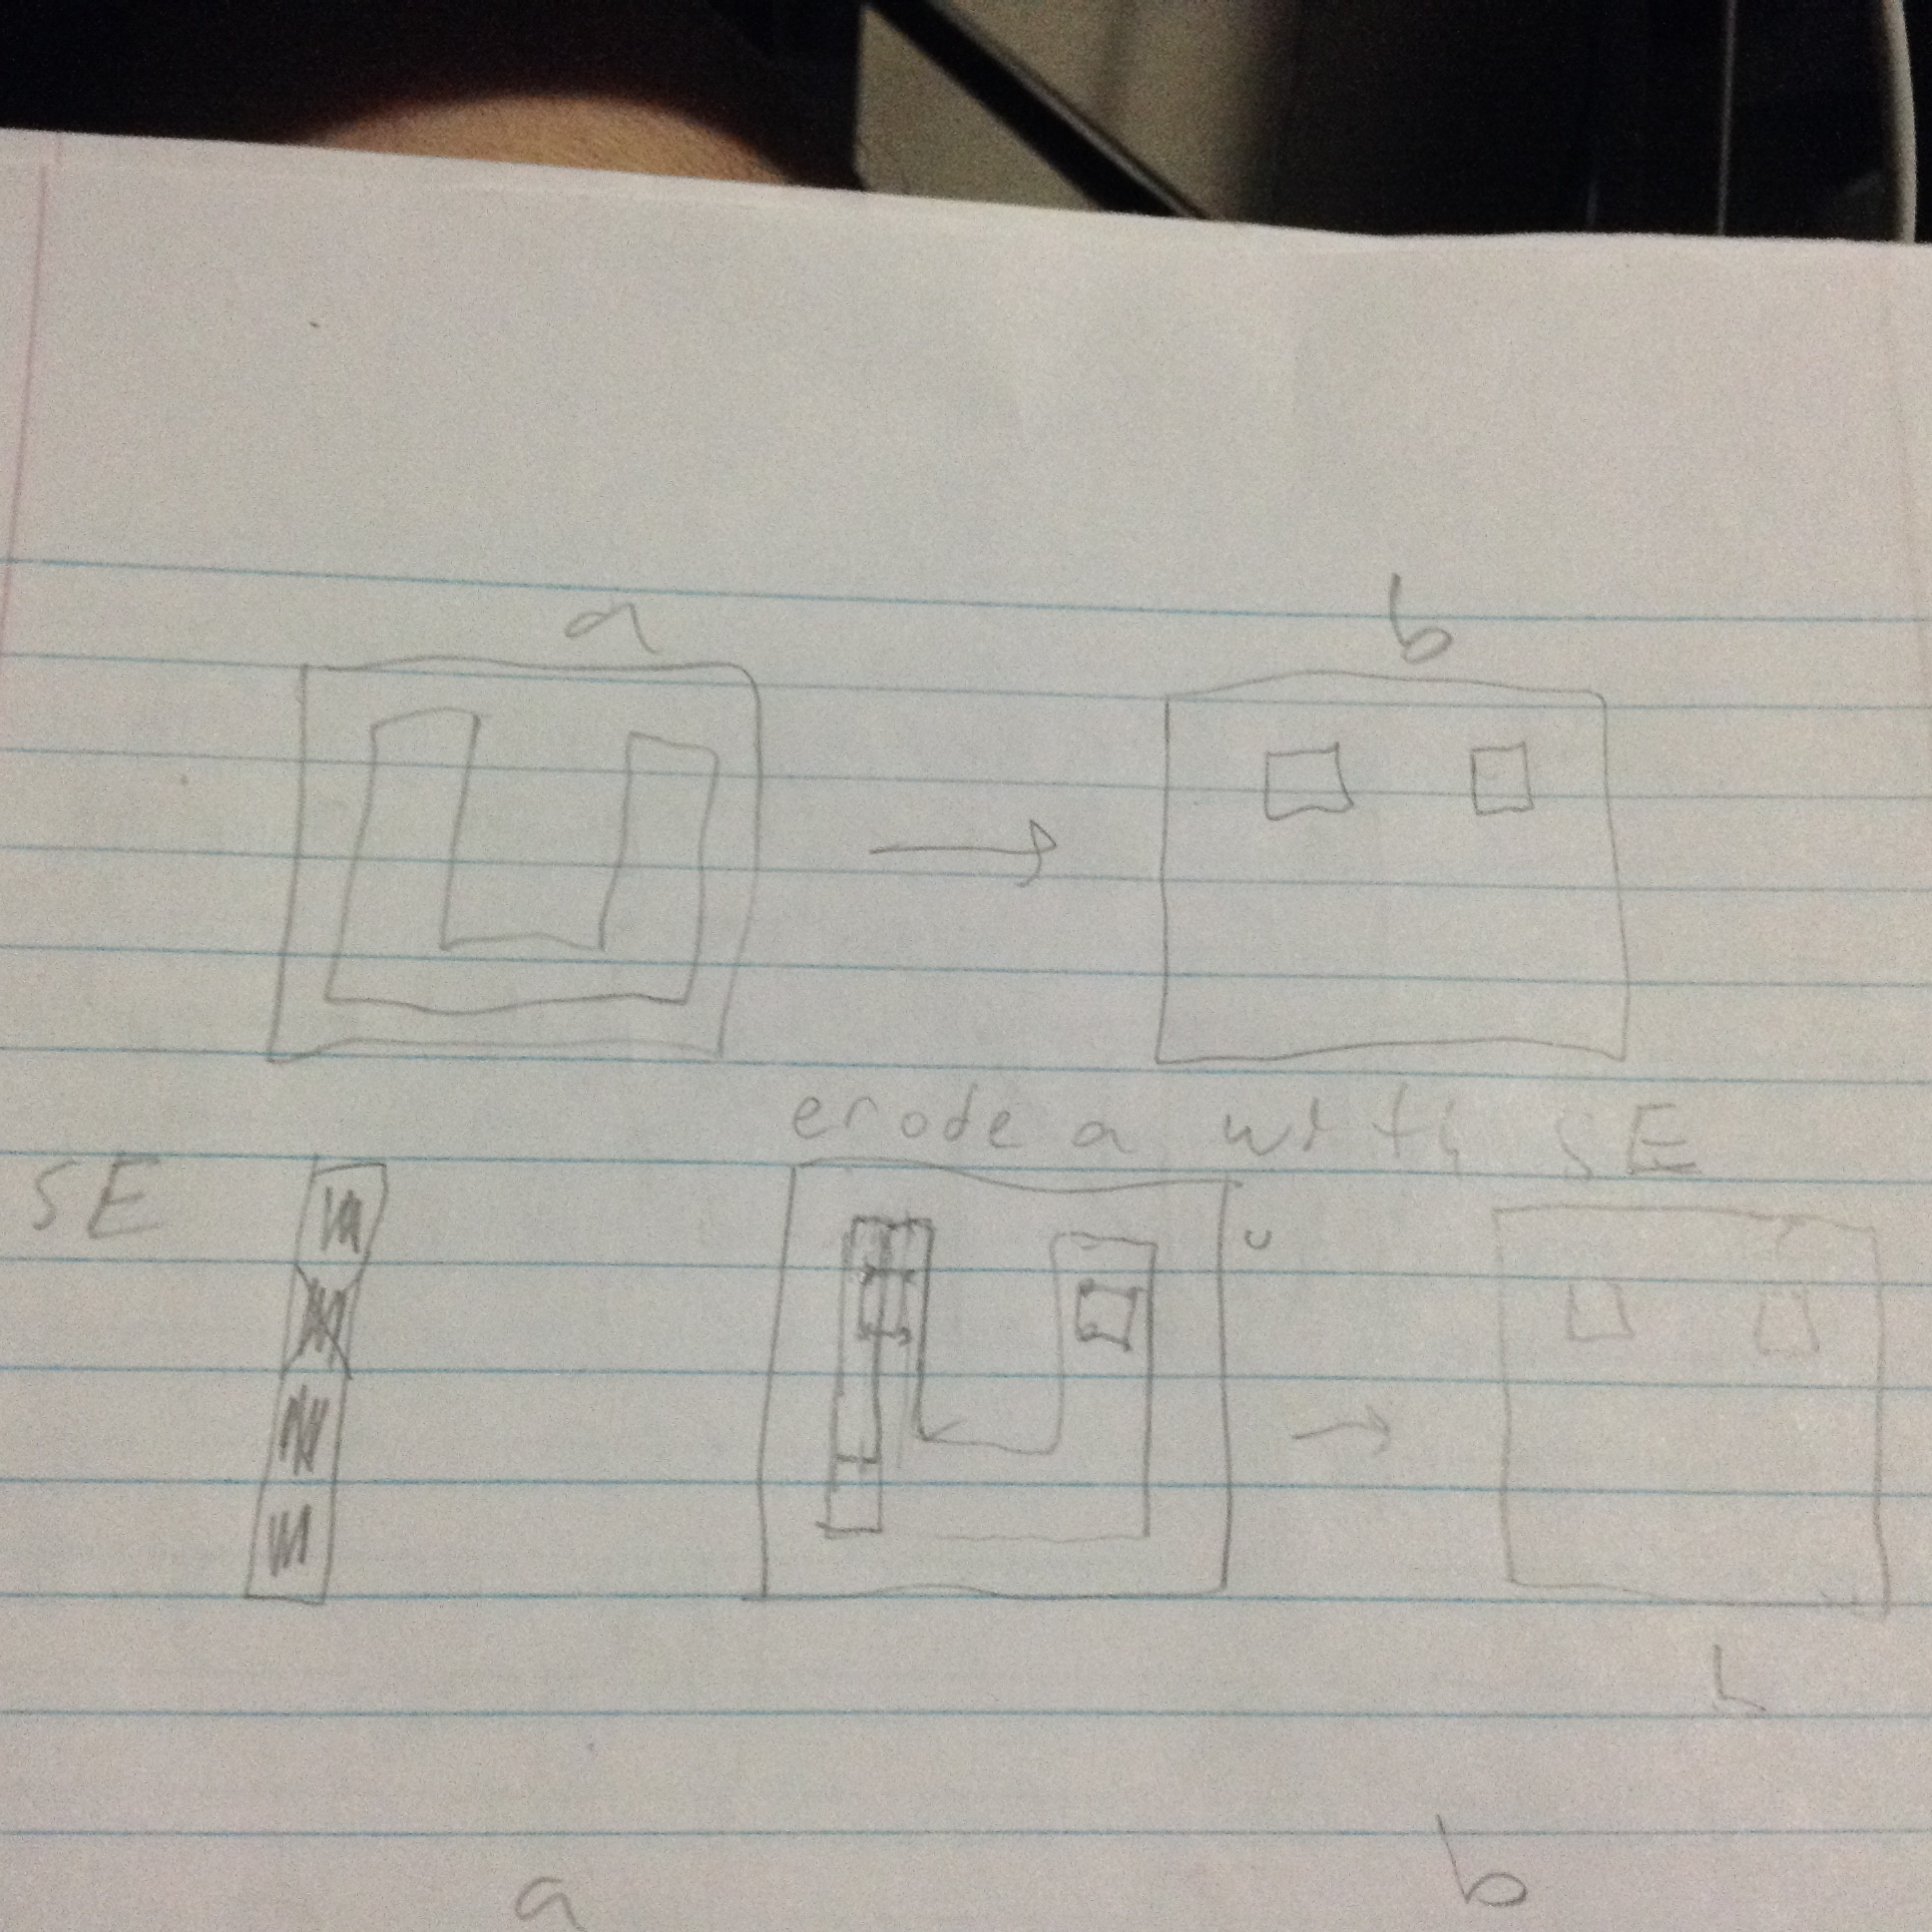
\includegraphics[width=\linewidth]{9.5/fig2.JPG}
	\end{figure}
	\subsection{Part c}
	\begin{figure}[H]
		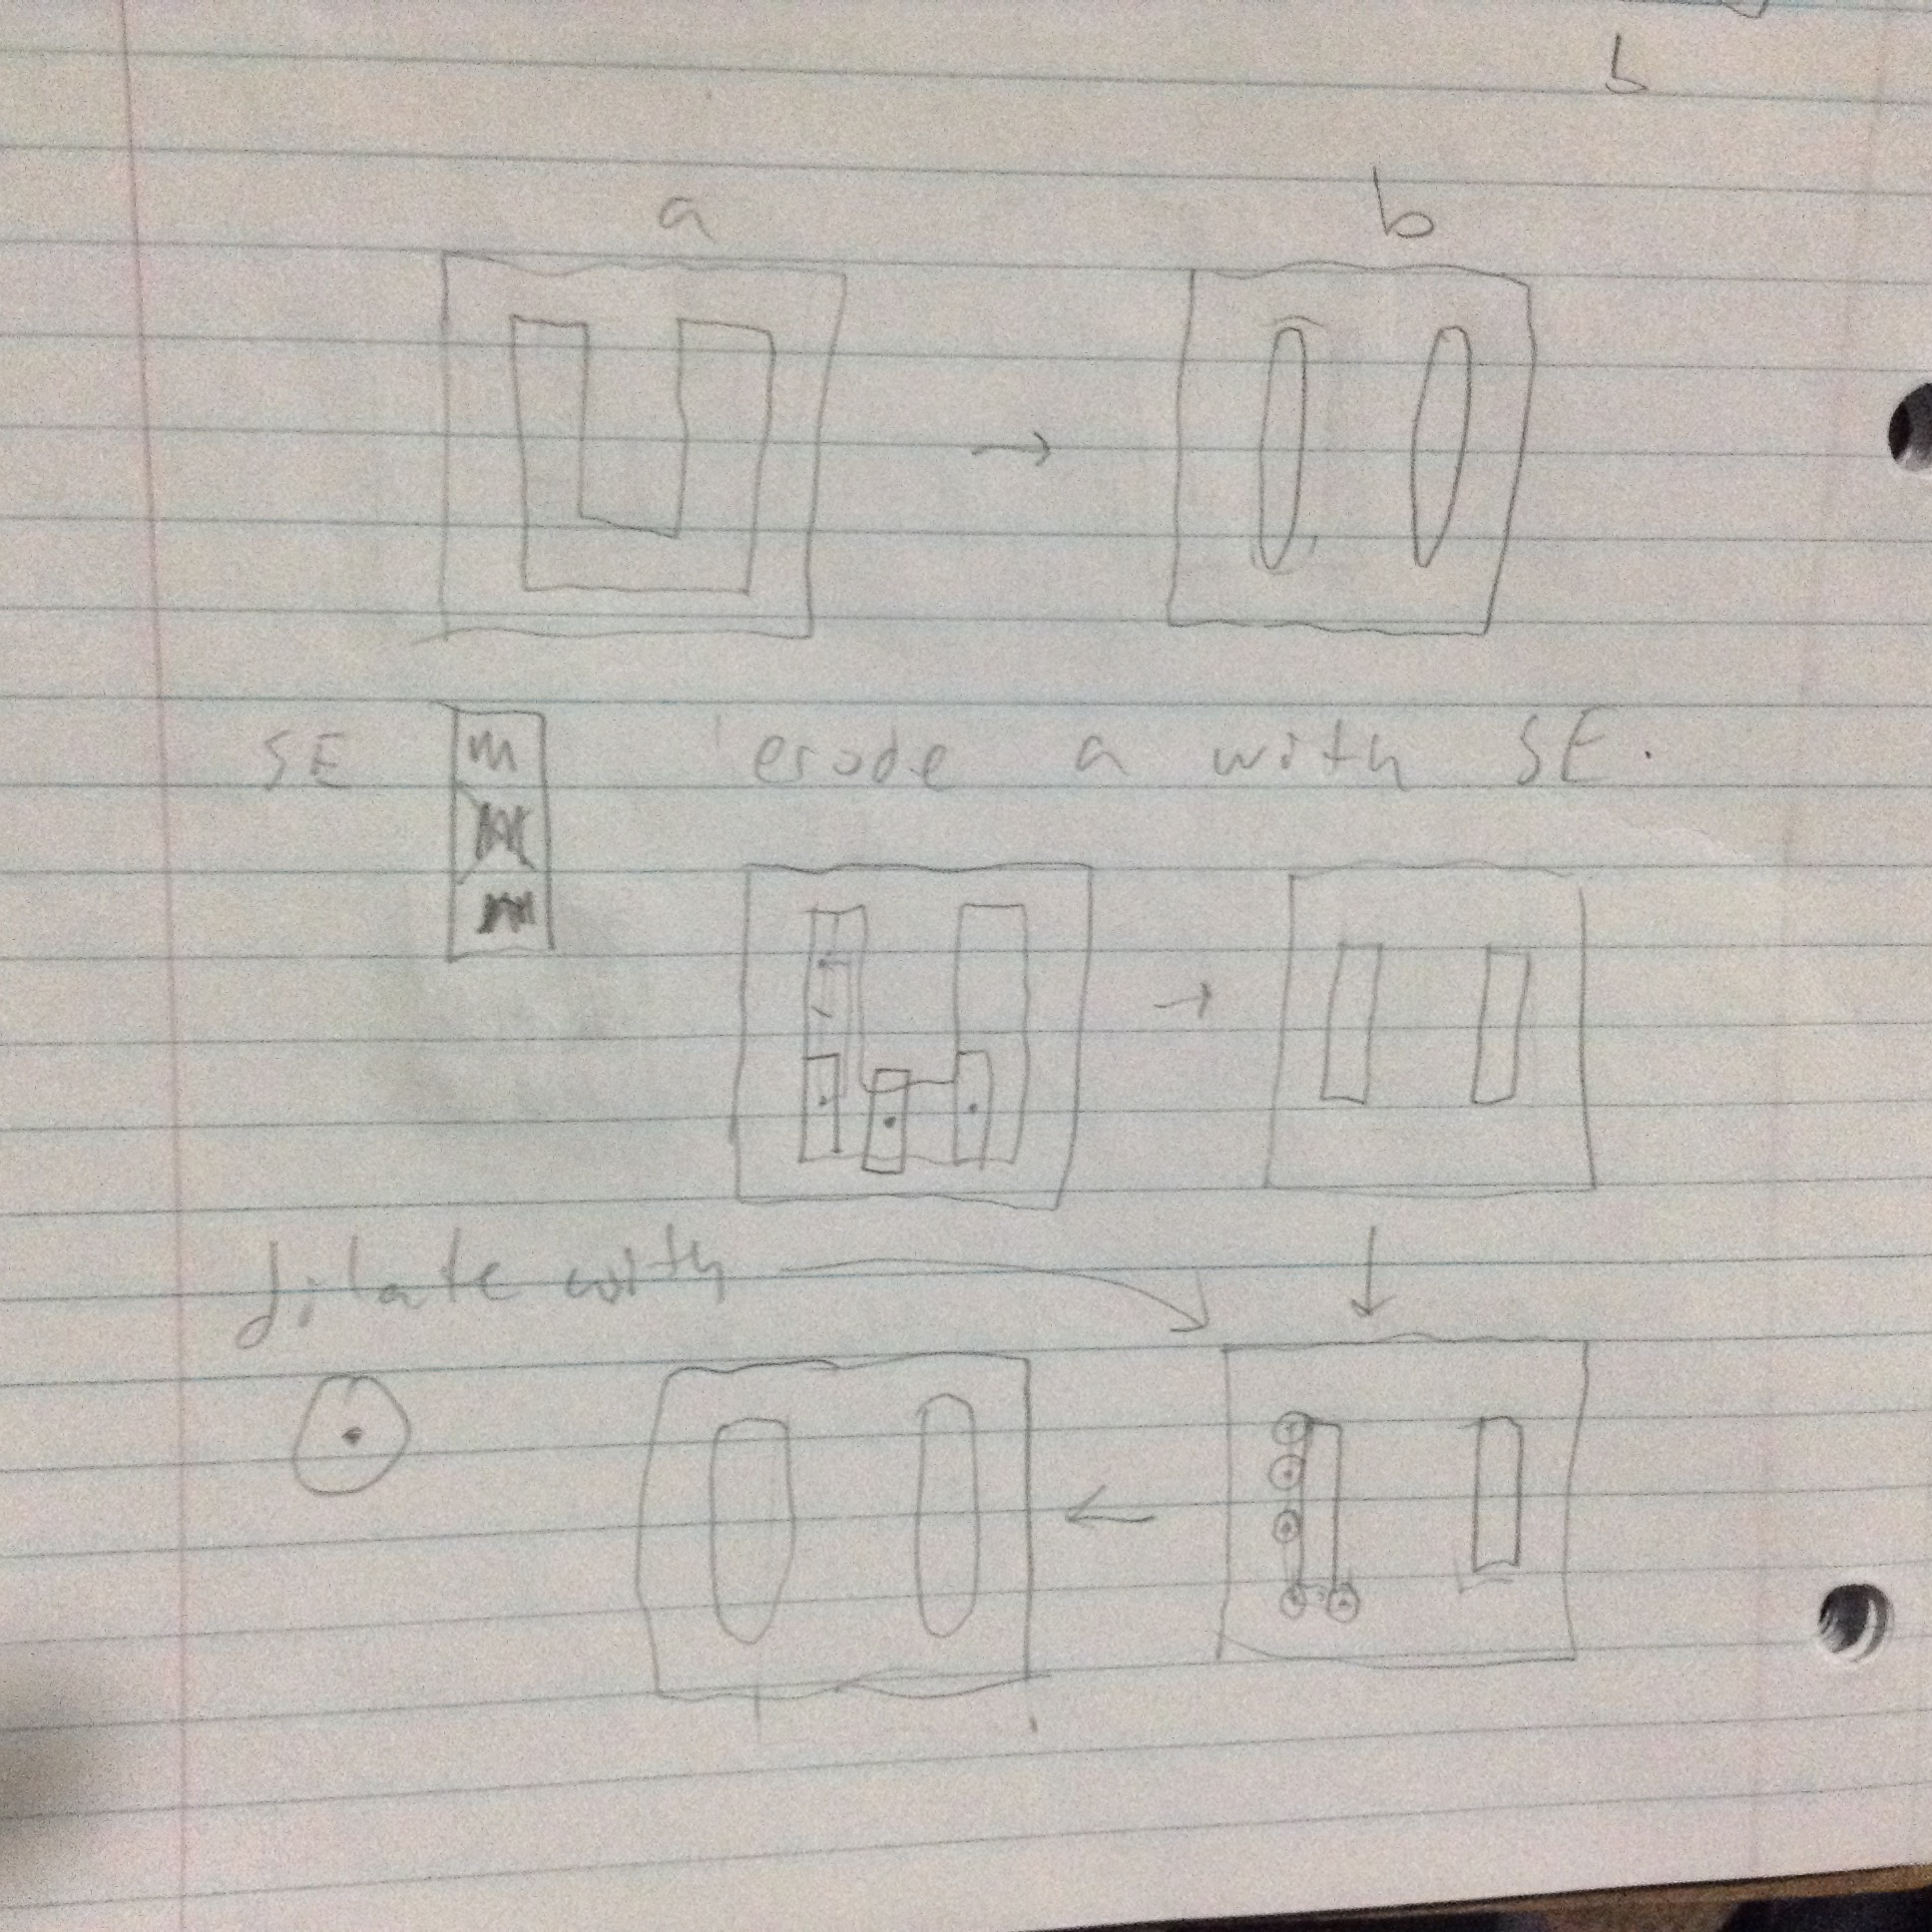
\includegraphics[width=\linewidth]{9.5/fig3.JPG}
	\end{figure}
	\subsection{Part d}
	\begin{figure}[H]
		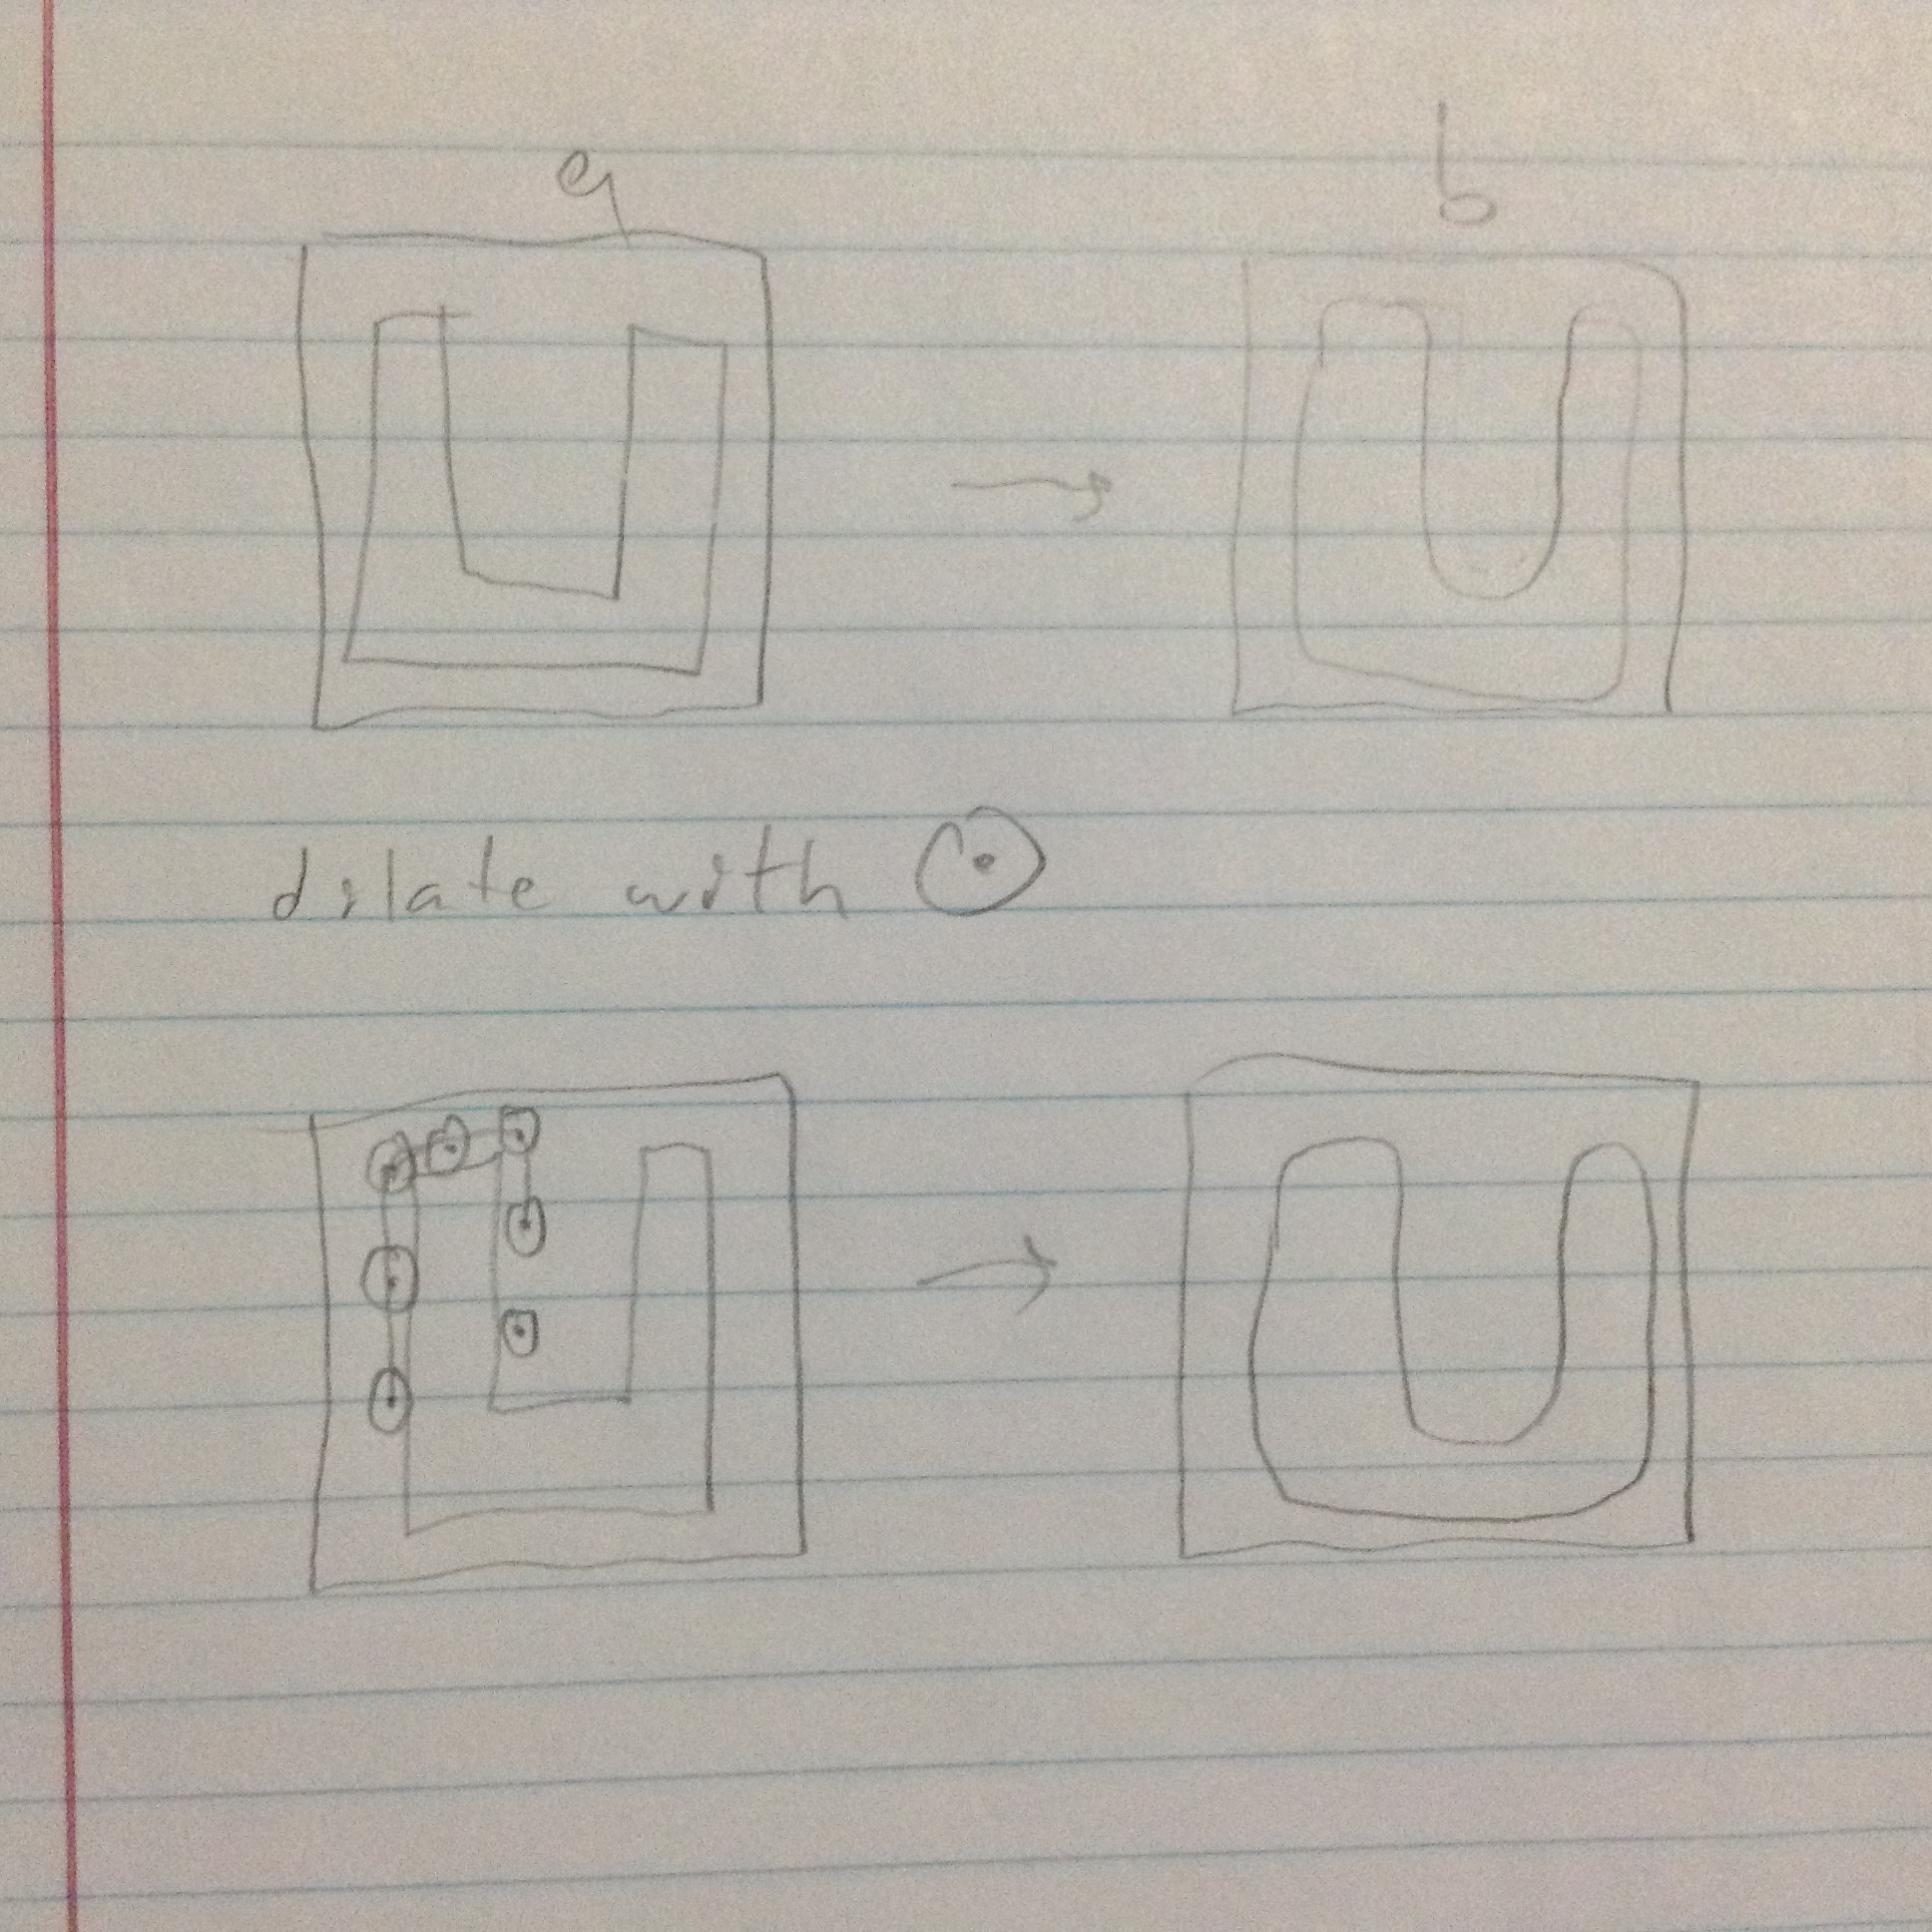
\includegraphics[width=\linewidth]{9.5/fig4.JPG}
	\end{figure}
	
	\newpage
	\section{Problem 9.6: Perform the morphological operations}
	\begin{figure}[H]
		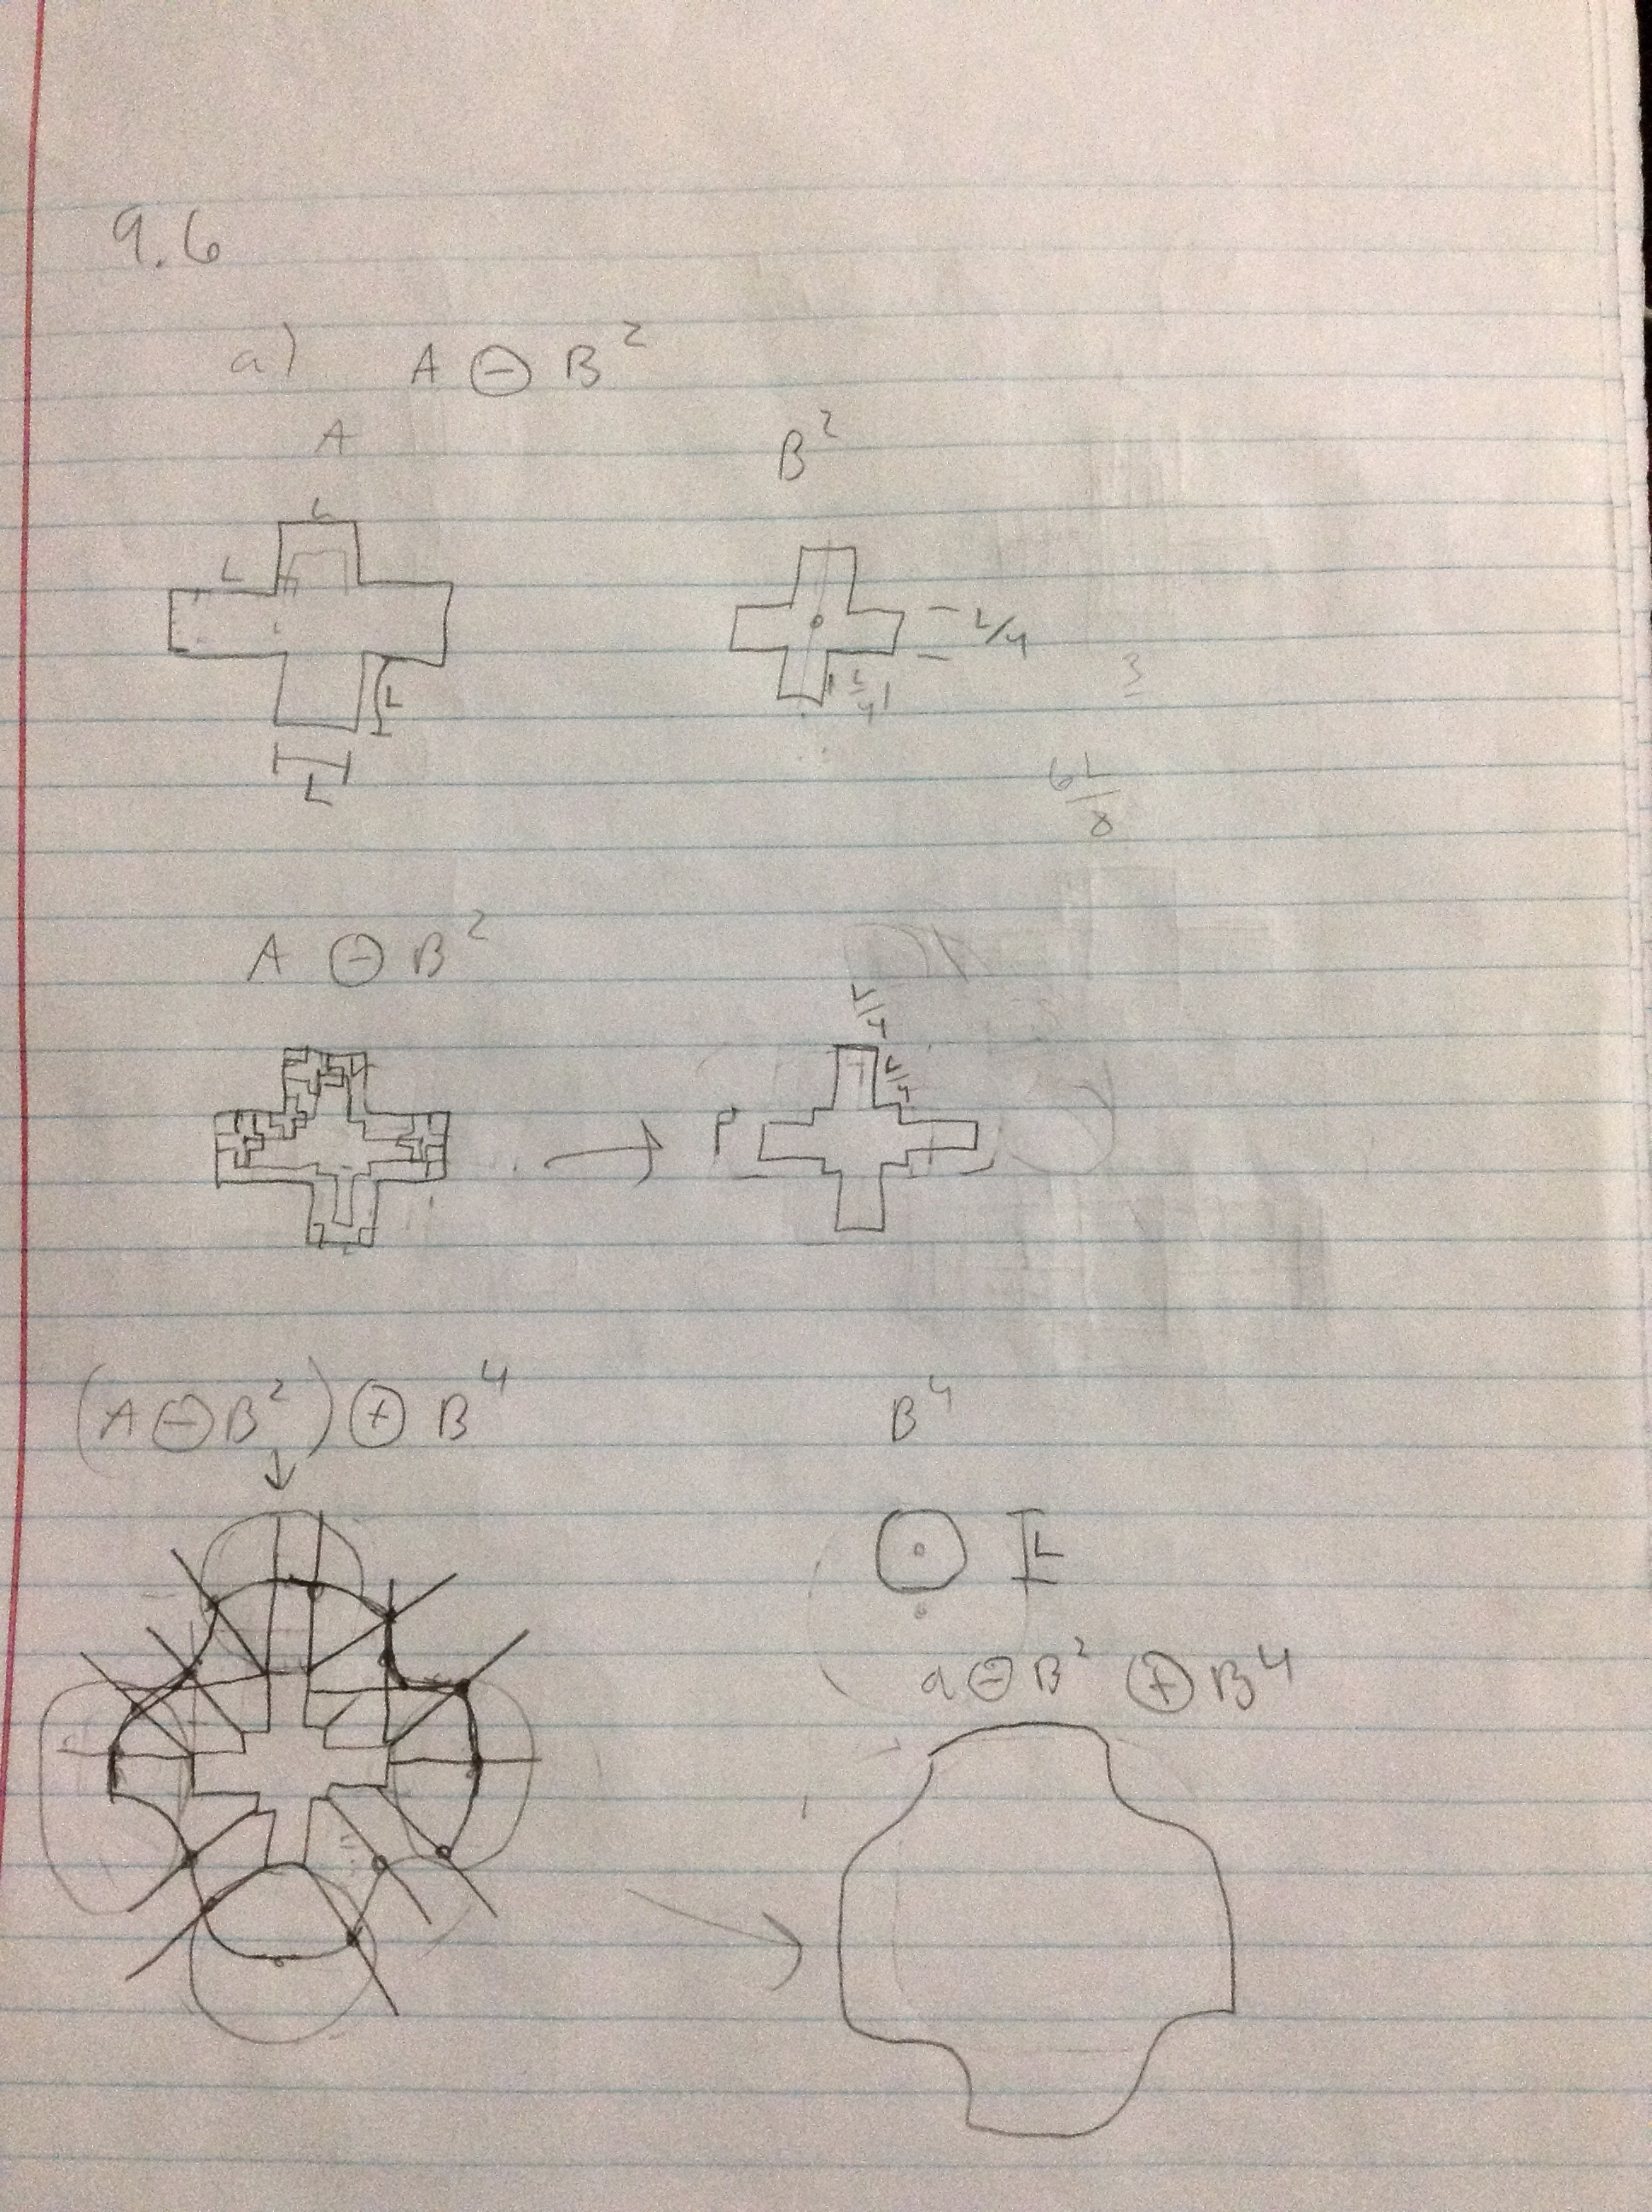
\includegraphics[width=\linewidth]{9.6/fig1.JPG}
	\end{figure}
	\subsection{Part b}
	\begin{figure}[H]
		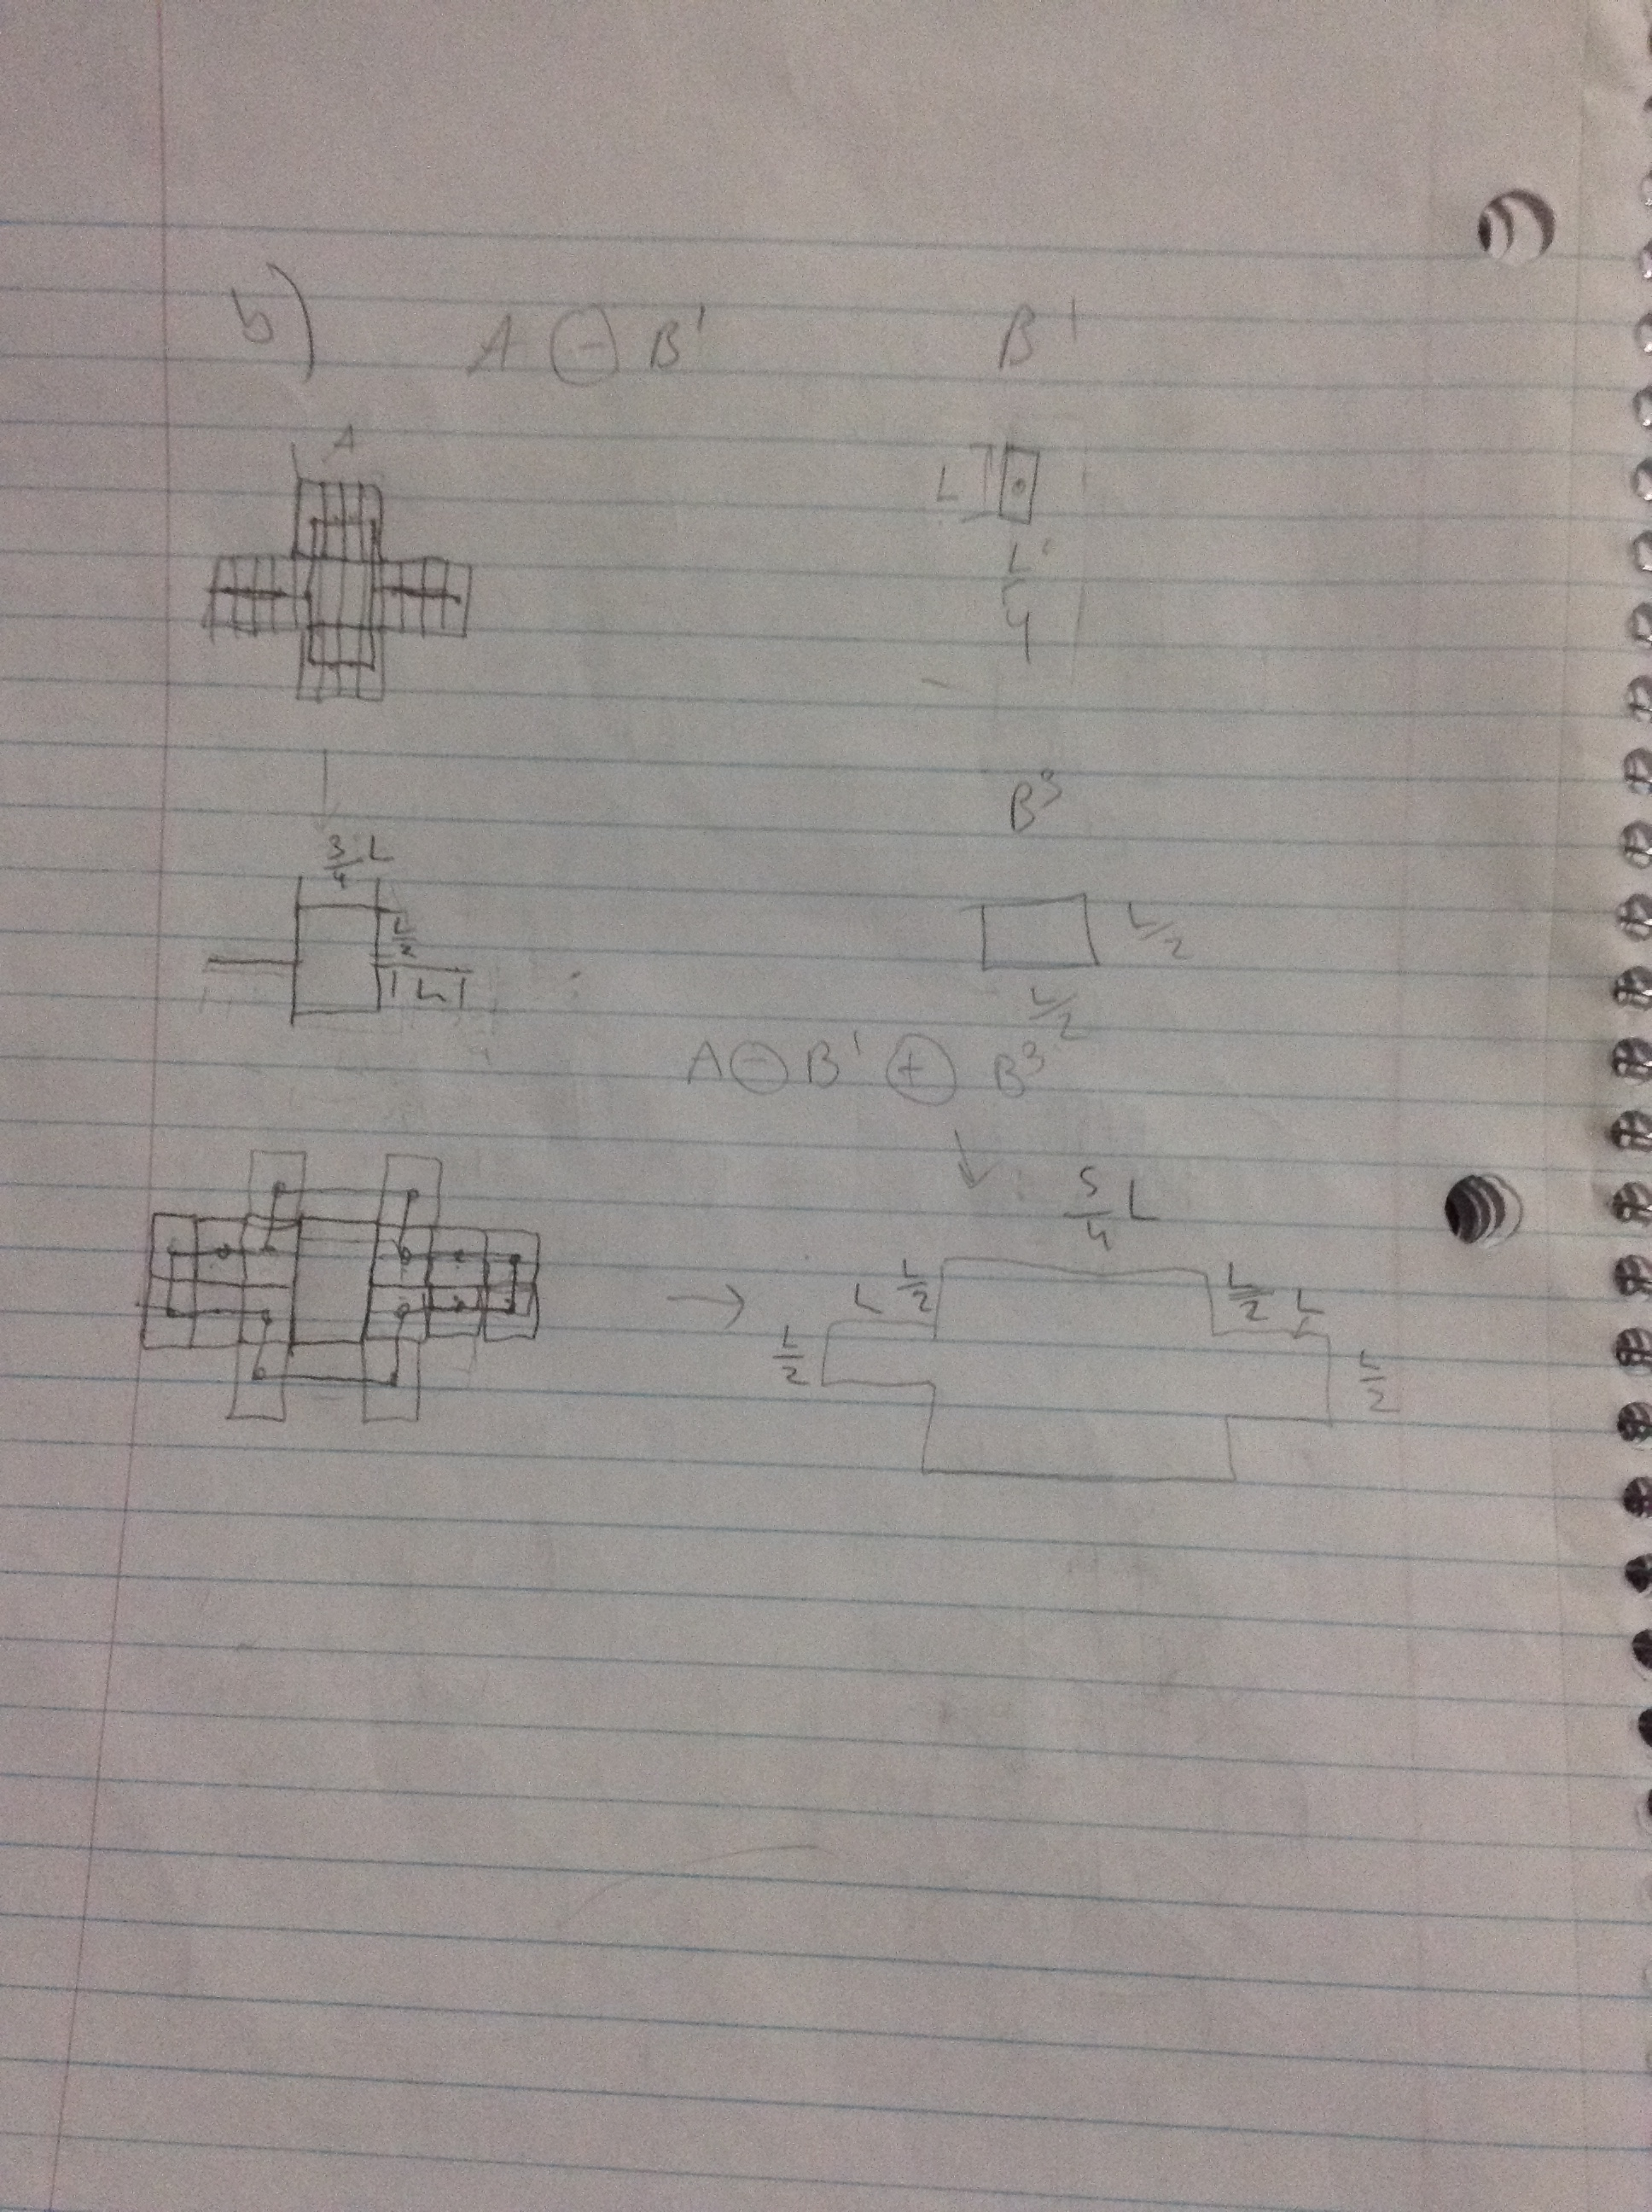
\includegraphics[width=\linewidth]{9.6/fig2.JPG}
	\end{figure}
	\subsection{Part c}
	\begin{figure}[H]
		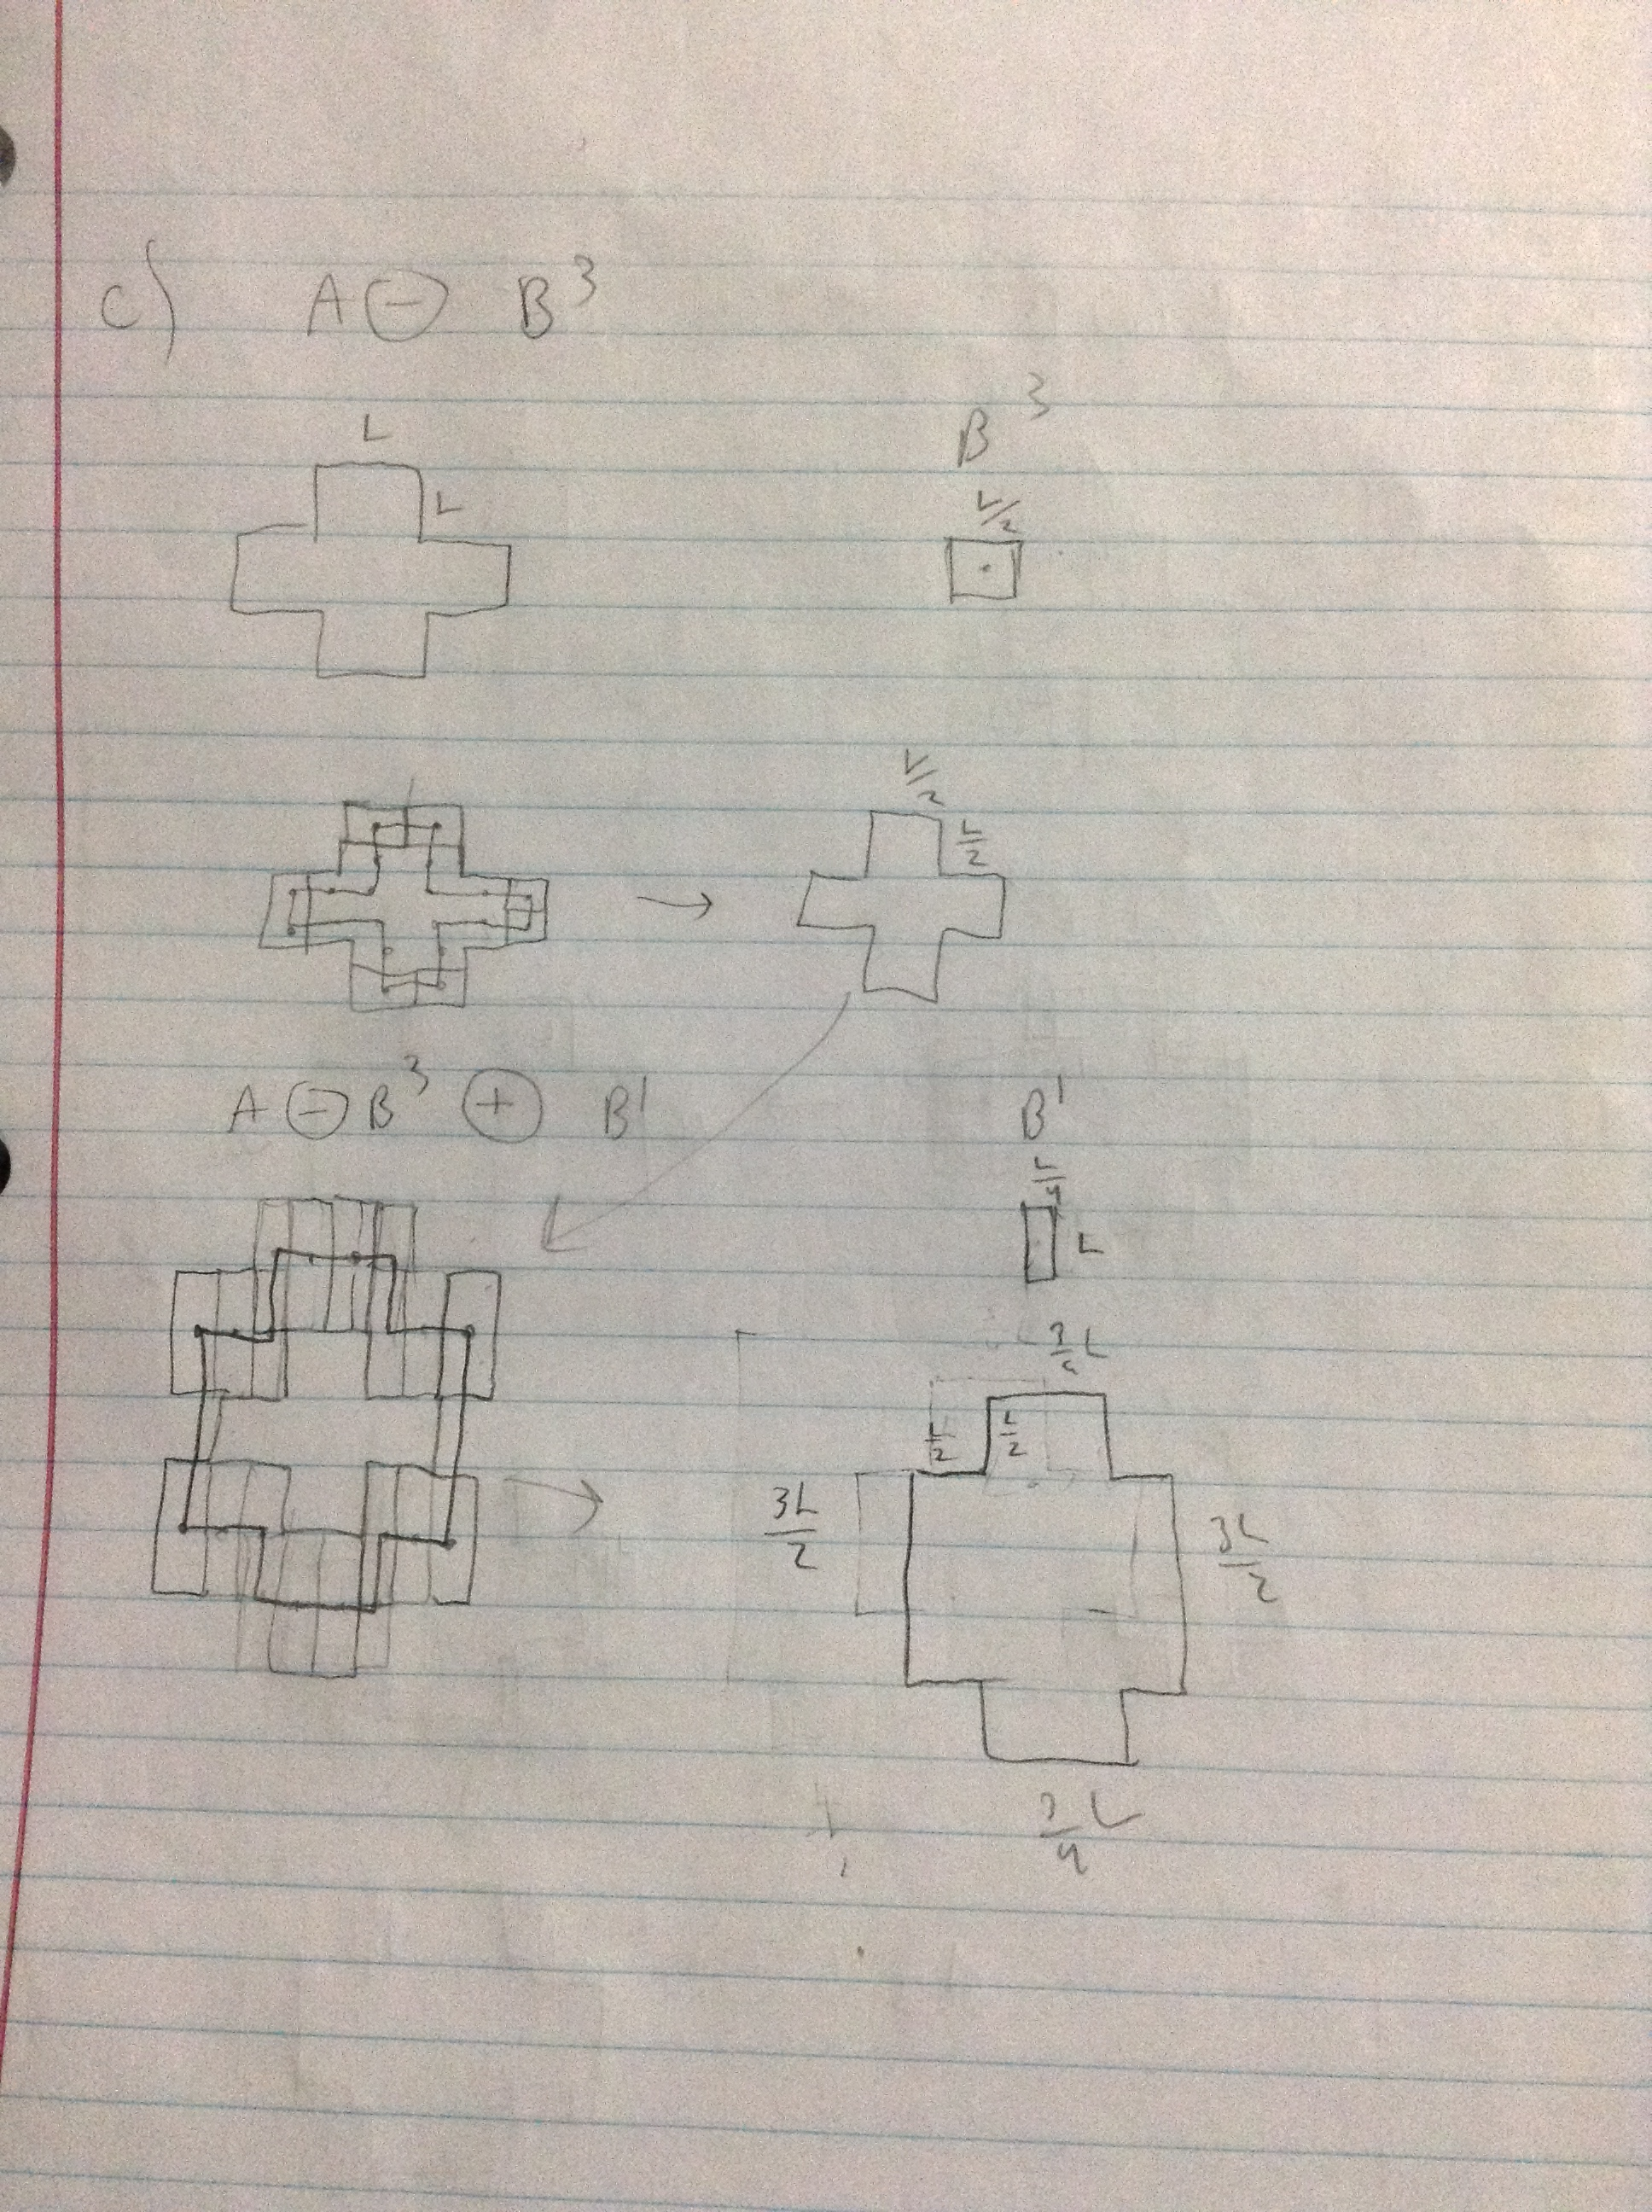
\includegraphics[width=\linewidth]{9.6/fig3.JPG}
	\end{figure}
	\subsection{Part d}
	\begin{figure}[H]
		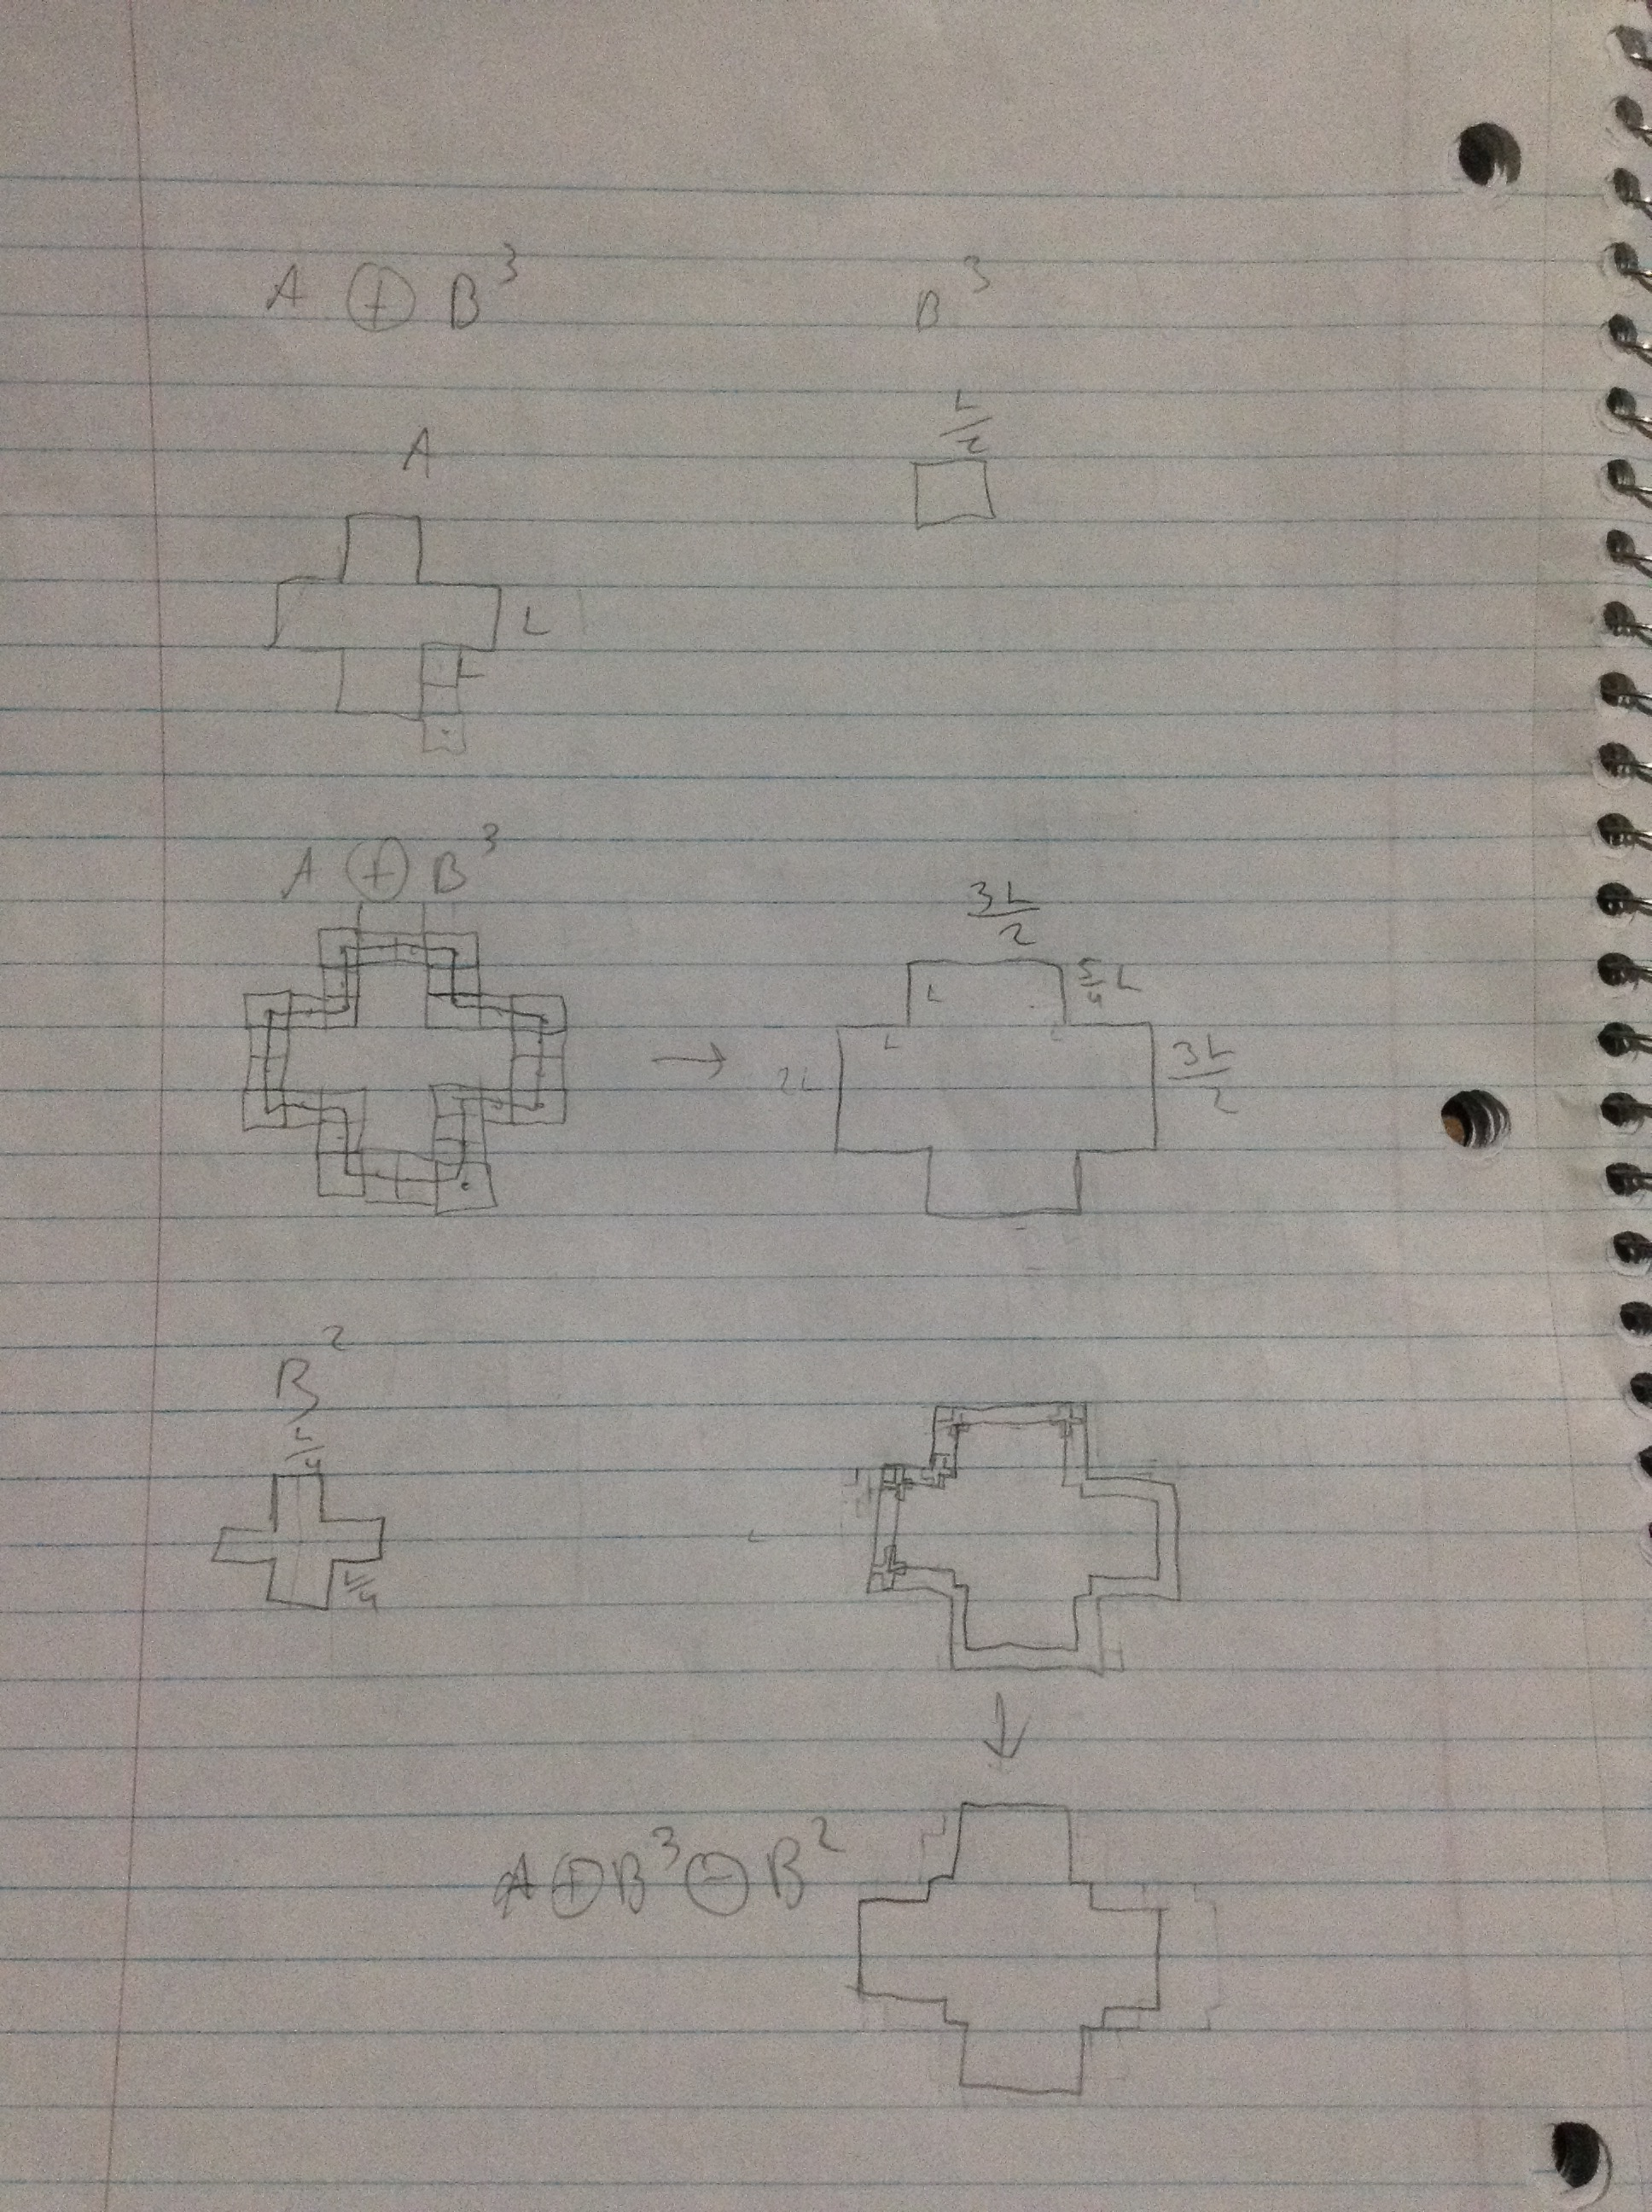
\includegraphics[width=\linewidth]{9.6/fig4.JPG}
	\end{figure}
	
	\newpage
	\section{Problem 9.19: Perform the hit or miss transform}
	There are no hits since the structural element is a lower case l.
	\begin{figure}[H]
		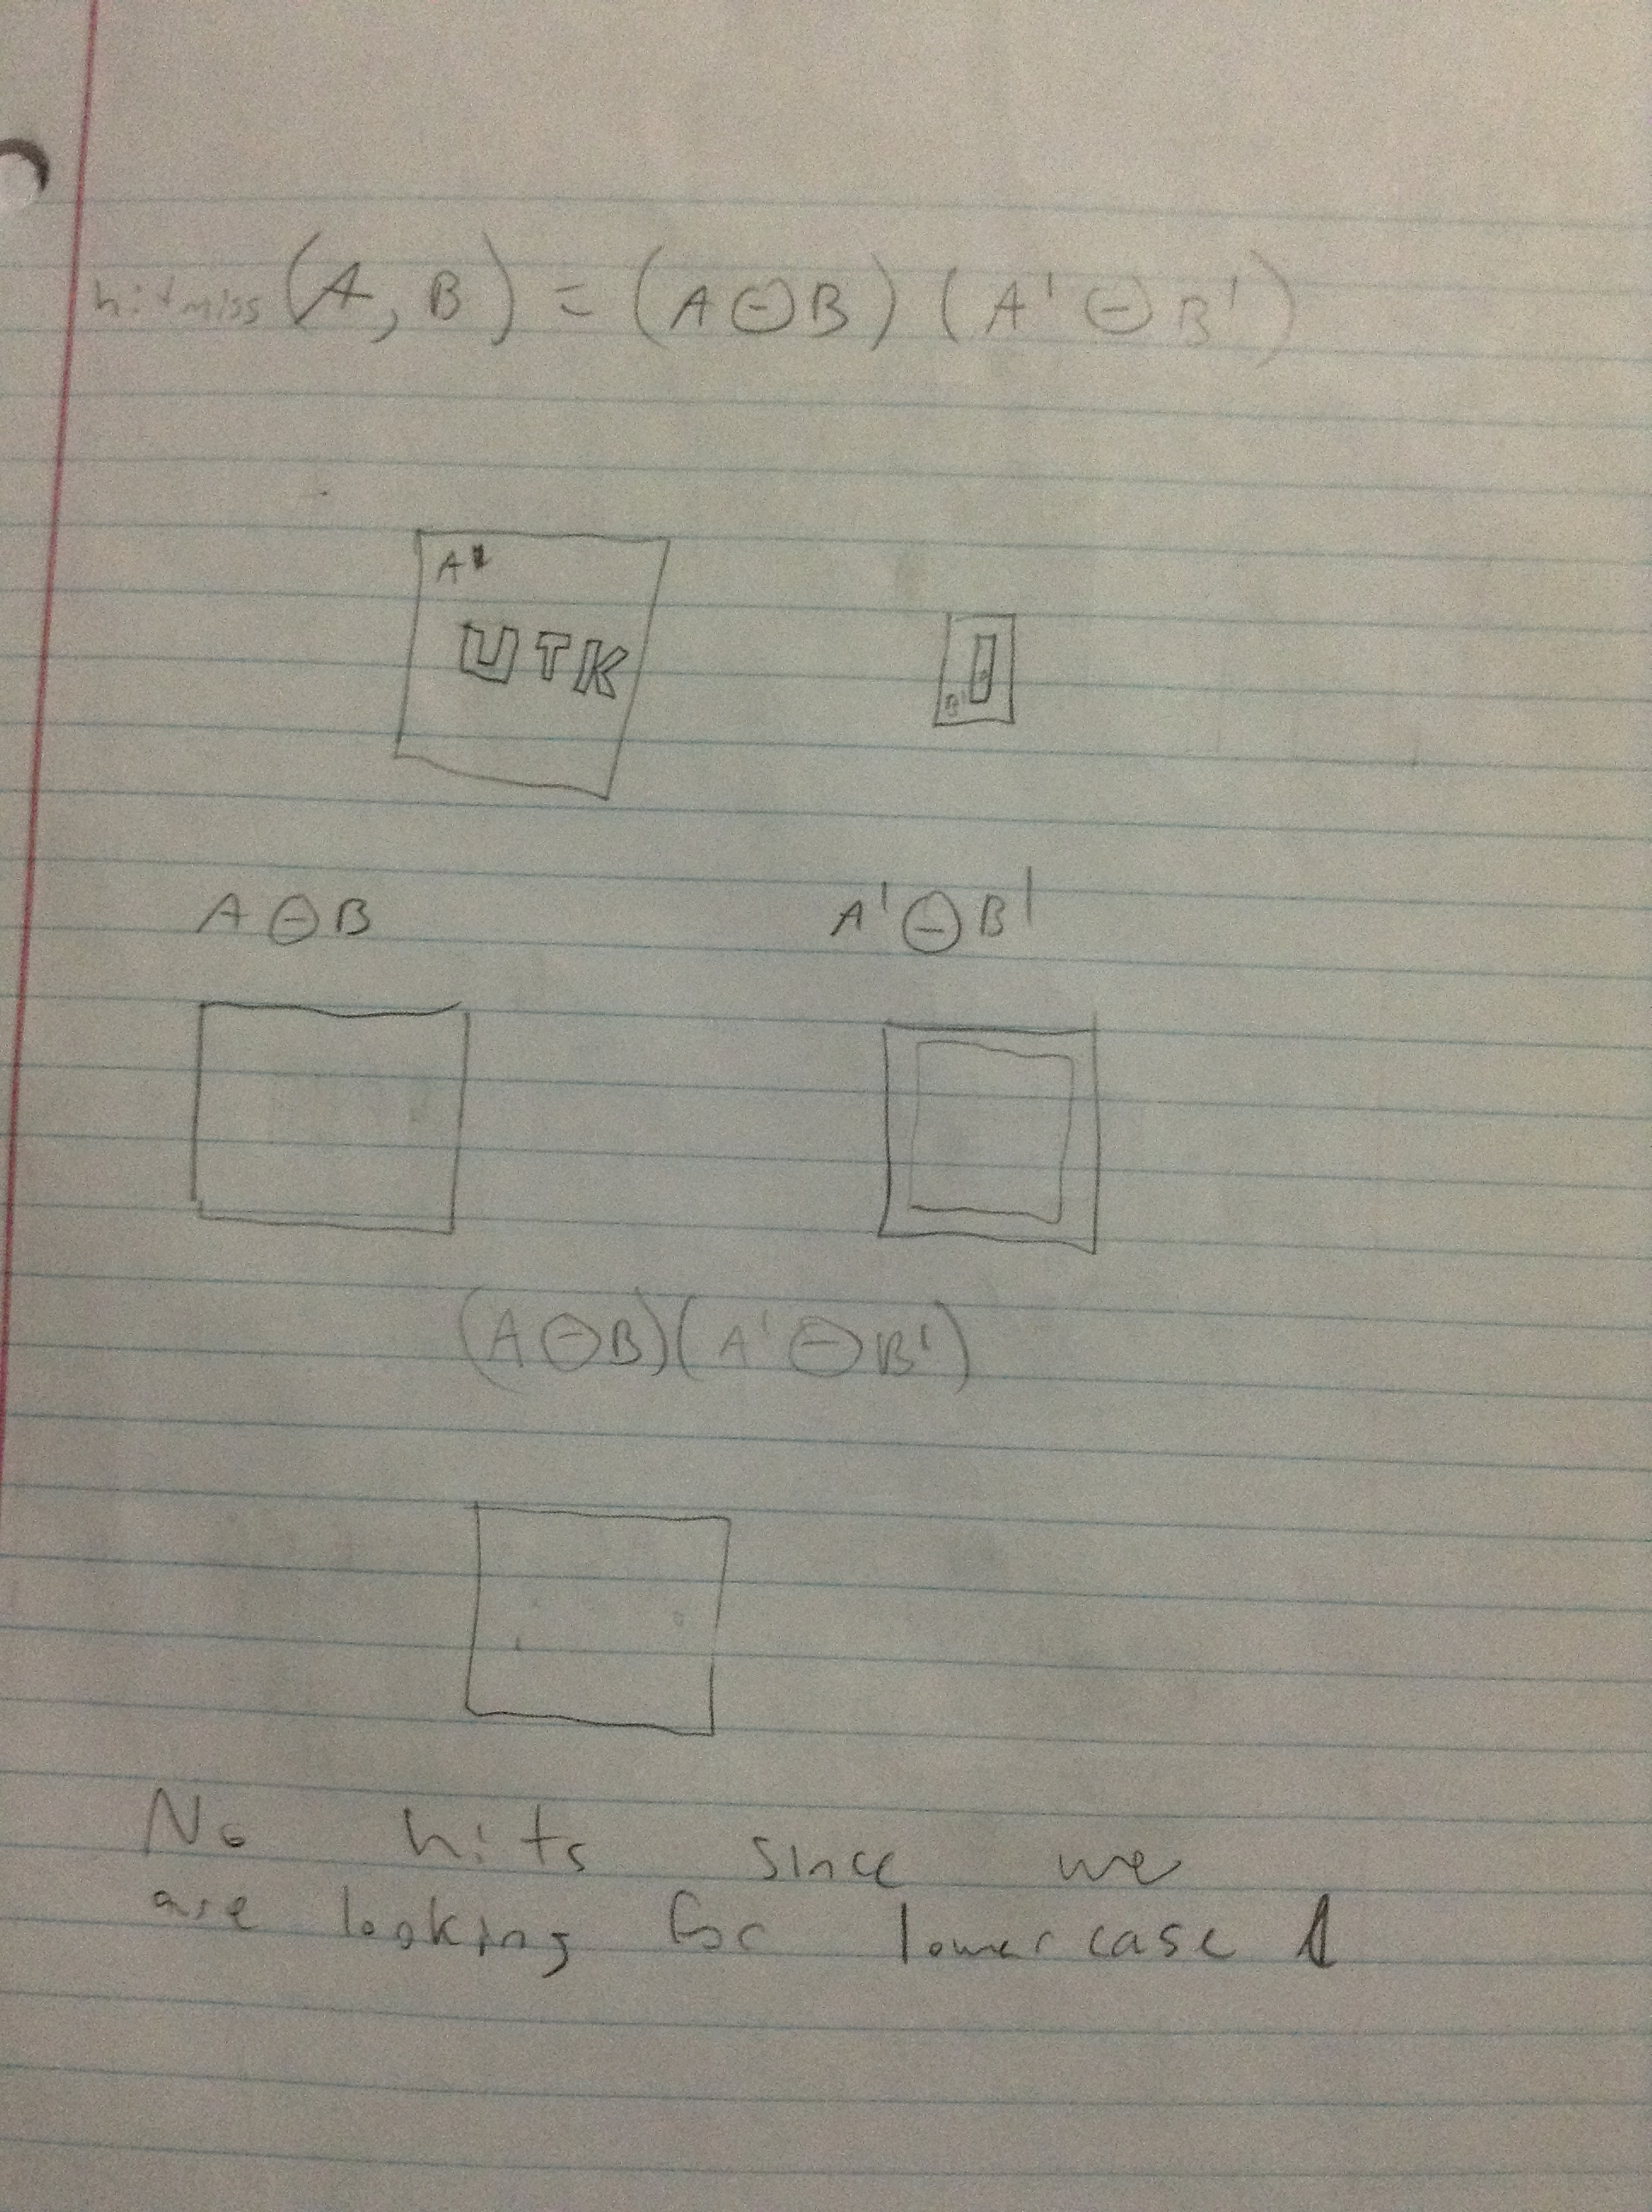
\includegraphics[width=\linewidth]{9.19/fig1.JPG}
	\end{figure}
	
	\newpage
	\section{Code}
	\subsection{6.17}
	\lstinputlisting[language=Octave]{6.17/partA/partA.m}
	\lstinputlisting[language=Octave]{6.17/partB/partB.m}
	\lstinputlisting[language=Octave]{6.17/partC/partC.m}
	\subsection{6.25}
	\lstinputlisting[language=Octave]{6.28/part1.m}
	\subsection{Problem 6}
	\lstinputlisting[language=Octave]{Q6/dilate.m}
\end{document}
